%%% Exemplo de utilização da classe ITA
%%%
%%%   por        Fábio Fagundes Silveira   -  ffs [at] ita [dot] br
%%%              Benedito C. O. Maciel     -  bcmaciel [at] ita [dot] br
%%%              Giovani Volnei Meinertz   -  giovani [at] ita [dot] br
%%%    	         Hudson Alberto Bode       -  bode [at] ita [dot]br
%%%    	         P. I. Braga de Queiroz    -  pi [at] ita [dot] br
%%%    	         Jorge A. B. Gripp         -  gripp [at] ita [dot] br
%%%    	         Juliano Monte-Mor         -  jamontemor [at] yahoo [dot] com [dot] br
%%%    	         Tarcisio A. B. Gripp      -  tarcisio.gripp [at] gmail [dot] com
%%%    	         
%%%
%%%  IMPORTANTE: O texto contido neste exemplo nao significa absolutamente nada.  :-)
%%%              O intuito aqui eh demonstrar os comandos criados na classe e suas
%%%              respectivas utilizacoes.
%%%
%%%  Tese.tex  2016-08-25
%%%  $HeadURL: http://www.apgita.org.br/apgita/teses-e-latex.php $
%%%
%%% ITALUS
%%% Instituto Tecnológico de Aeronáutica --- ITA, Sao Jose dos Campos, Brasil
%%%                   http://groups.yahoo.com/group/italus/
%%% Discussion list: italus {at} yahoogroups.com
%%%
%++++++++++++++++++++++++++++++++++++++++++++++++++++++++++++++++++++++++++++++
% Para alterar o TIPO DE DOCUMENTO, preencher a linha abaixo \documentclass[?]{?}
%   \documentclass[tg]{ita}			= Trabalho de Graduacao
%   \documentclass[tgfem]{ita}	= Para Engenheiras
%   								msc     		= Dissertacao de Mestrado
%   								mscfem   		= Para Mestras
%   								dsc      		= Tese de Doutorado
%   								dscfem   		= Para Doutoras
%   								quali    		= Exame de Qualificacao
%   								qualifem 		= Exame de Qualificacao para Doutoras
% Para 'Draft Version'/'Versao Preliminar' com data no rodape, adicionar 'dv':
%   \documentclass[dsc, dv]{ita} 
% Para trabalhos em Inglês, adicionar 'eng':
%   \documentclass[dsc, eng]{ita}
%		\documentclass[dsc, eng, dv]{ita}
%++++++++++++++++++++++++++++++++++++++++++++++++++++++++++++++++++++++++++++++
\documentclass[tg, eng, dv]{ita}    % ITA.cls based on standard book.cls 
% Quando alterar a classe, por exemplo de [msc] para [msc, eng]) rode mais uma vez o botão BUILD OUTPUT caso haja erro
\usepackage{ae}
\usepackage{graphicx}
\usepackage{epsfig}
\usepackage{amsmath}

\DeclareMathOperator*{\argmax}{arg\,max}
\DeclareMathOperator*{\argmin}{arg\,min}
\usepackage{amssymb} 
\usepackage{subfig}
\usepackage{multirow}
\usepackage{float}
\usepackage{algorithm}
\usepackage{algorithmic}


\newtheorem{definition}{Definition}    
    
\newcommand{\bvec}[1]{\mathrm{\mathbf{#1}}}    
        

%++++++++++++++++++++++++++++++++++++++++++++++++++++++++++++++++++++++++++++++
% Espaçamento padrão de todo o documento
%++++++++++++++++++++++++++++++++++++++++++++++++++++++++++++++++++++++++++++++
\onehalfspacing

%singlespacing Para um espaçamento simples
%onehalfspacing Para um espaçamento de 1,5
%doublespacing Para um espaçamento duplo

%++++++++++++++++++++++++++++++++++++++++++++++++++++++++++++++++++++++++++++++
% Identificacoes (se o trabalho for em inglês, insira os dados em inglês)
% Para entradas abreviadas de Professora (Profa.) em português escreva: Prof$^\textnormal{a}$.
%++++++++++++++++++++++++++++++++++++++++++++++++++++++++++++++++++++++++++++++
\course{Computer Engineering} % Programa de PG ou Curso de Graduação

% Autor do trabalho: Nome Sobrenome
\authorgender{masc}                     %sexo: masc ou fem
\author{Luckeciano}{Carvalho Melo}
\itaauthoraddress{H8A St., 113}{12.228-460}{São José dos Campos--SP}

% Titulo da Tese/Dissertação
\title{A Deep Reinforcement Learning Method for Humanoid Kick Motion}

% Orientador
\advisorgender{masc}                    % masc ou fem
\advisor{Prof.~Dr.}{Adilson Marques da Cunha}{ITA}

% Coorientador (Caso não haja coorientador, colocar ambas as variáveis \coadvisorgender e \coadvisor comentadas, com um % na frente)
\coadvisorgender{fem}									% masc ou fem
\coadvisor{Prof. Dr.}{Marcos R. O. de A. Máximo}{ITA}

% Pró-reitor da Pós-graduação
%\bossgender{masc}												% masc ou fem
%boss{Prof.~Dr.}{John von Neumann}

%Coordenador do curso no caso de TG
\bosscoursegender{fem}									% masc ou fem
\bosscourse{Prof$^\textnormal{a}$.Dr$^\textnormal{a}$.}{Cecília César}

% Palavras-Chaves informadas pela Biblioteca -> utilizada na CIP
\kwcip{Deep Reinforcement Learning}
\kwcip{Robotics}
\kwcip{Artificial Intelligence}

% membros da banca examinadora

\examiner{Prof. Dr.}{Adilson Marques da Cunha}{}{ITA}
\examiner{Prof. Dr.}{Marcos R. O. de A. Máxim}{}{ITA}
\examiner{Prof. Dr.}{Paulo André L. de Castro}{}{ITA}

% Data da defesa (mês em maiúsculo, se trabalho em inglês, e minúsculo se trabalho em português) 
\date{12}{JUNE}{2018}

% Número CDU - (somente para TG)
\cdu{621.38}

% Glossario
\makeglossary
\frontmatter

\begin{document}
% Folha de Rosto e Capa para o caso do TG
\maketitle
% * <luckeciano@hotmail.com> 2018-08-08T03:26:41.936Z:
%
% ^.
% * <luckeciano@hotmail.com> 2018-08-08T03:26:40.755Z:
%
% ^.
% Dedicatoria: Nao esqueca essa secao  ... :-)
%\begin{itadedication}

 
%\end{itadedication}

% Agradecimentos
%\begin{itathanks}
%Macaco

%\end{itathanks}

% Epígrafe
%\thispagestyle{empty}
%\ifhyperref\pdfbookmark[0]{\nameepigraphe}{epigrafe}\fi
%\begin{flushright}
%\begin{spacing}{1}
%\mbox{}\vfill
%{\sffamily\itshape
%``If I have seen farther than others,\\
%it is because I stood on the shoulders of giants.''\\}
%--- \textsc{Sir~Isaac Newton}
%\end{spacing}
%\end{flushright}

% Resumo
%\begin{abstract}
%\noindent
%Controlling a high degrees of freedom humanoid robot is acknowledged as one of the hardest problems in Robotics. Due to the lack of mathematical models, an approach frequently employed is to rely on human intuition to design keyframe movements by hand, usually aided by graphical tools. In this paper, we propose a learning framework based on neural networks in order to mimic humanoid robot movements. The developed technique does not make any assumption about the underlying implementation of the movement, therefore both keyframe and model-based motions may be learned. The framework was applied in the RoboCup 3D Soccer Simulation domain and promising results were obtained using the same network architecture for several motions, even when copying motions from another teams.
%\end{abstract}

% Abstract
\begin{englishabstract}
\noindent
Controlling high degrees of freedom for humanoid robot is acknowledged as one of the hardest problems in Robotics. Due to the lack of mathematical models, an approach frequently employed is to rely on human intuition to design keyframe movements by hand, usually aided by graphical tools. In this work, we firstly propose some methods based upon neural networks in order to imitate keyframe motions. Then, we  propose a learning framework that not just imitates but also optimizes humanoid robot movement towards a task using Deep Reinforcement Learning. The developed technique does not make any assumption about the underlying implementation of the movement. The framework was applied in the RoboCup 3D Soccer Simulation domain and was able to improve the accuracy of given kick motion from 69\% to 92\% and also improved kick general distance.
\end{englishabstract}

% Lista de figuras
\listoffigures %opcional

% Lista de tabelas
\listoftables %opcional

% Lista de abreviaturas
%\listofabbreviations
%\begin{longtable}{ll}
ACER & Actor-Critic with Experience Replay \\
A2C & Advantage-Actor-Critic \\
API & Application Programming Interface \\
BGC & Batch Gradient Descent \\
CPU & Central Processor Unit \\
CMA-ES & Covariance Matrix Adaptation Evolution Strategy \\
CEM & Cross-Entropy Method \\
DDPG & Deep Deterministic Policy Gradient \\
DAG & Directed Acyclic Graph \\
DPPO & Distributed Proximal Policy Optimization \\
DP & Dynamic Programming \\
GAE & Generalized Advantage Estimation \\
GAIL & Generative Adversarial Imitation Learning \\
GUI & Graphical User Interface \\
GPU & Graphic Processor Unit \\
HC & Hill Climbing \\
HER & Hindsight Experience Replay \\
HLM & Hybrid Learning Model \\
HTTP & Hypertext Transfer Protocol \\
KL & Kullback-Leibler \\
MDP & Markov Decision Process \\
MP & Markov Process \\
MRP & Markov Reward Process \\
ML & Machine Learning \\
MuJoCo & Multi-Joint dynamics with Contact \\
ODE & Open Dynamics Engine \\
PPO & Proximal Policy Optimization \\
ReLU & Rectified Linear Unit \\
RL & Reinforcement Learning \\
RISD & Reinforcement with Initial State Distribution \\
RET & Reinforcement with Early Termination \\
RNR & Reinforcement with Naive Reward \\
RRR & Reinforcement with Reference Reward \\
RPC & Remote Procedure Call \\
SIMD & Single Instruction Multiple Data \\
SGD & Stochastic Gradient Descent \\
TPU & Tensor Processor Unit \\
TCP & Transmission Control Protocol \\
TRPO & Trusted Region Policy Optimization \\
ZMP & Zero Moment Point \\

\end{longtable}

 %opcional

% Lista de simbolos
%\listofsymbols
%\begin{longtable}{ll}
{\bf Sets} \\
$K$ & Keyframe set \\
$\mathbb{R}$ & The set of real numbers \\
$\mathbb{A}$ & A set \\
\\
{\bf Numbers and Arrays} \\
$\boldsymbol{x}$ & A vector $\boldsymbol{x}$ \\
$A$ & Matrix $A$ \\
$\boldsymbol{I}$ & Identity matrix \\
$\boldsymbol{X}$ & Tensor $\boldsymbol{X}$ \\
\\

{\bf Linear Algebra Operations} \\
$\boldsymbol{A}^{T}$ & Transpose of matrix $\boldsymbol{A}$ \\
$\lVert \boldsymbol{x} \rVert$ & $L^{2}$ norm of $\boldsymbol{x}$ \\
$\boldsymbol{a} \odot \boldsymbol{b}$ & Element-wise multiplication of vectors $a$ and $b$ \\

\\

{\bf Calculus} \\
$\frac{dy}{dx}$ & Derivative of $y$ w.r.t $x$ \\
$\frac{\partial{J}}{\partial{x}}$ & Partial derivative of $J$ w.r.t $x$ \\
$\nabla_{\boldsymbol{X}}z$ & Gradient of $z$ w.r.t $\boldsymbol{X}$ \\
$\lim_{k \rightarrow b} a$ & Limit of $a$ when $k$ tends to $b$ \\

\\

{\bf Probabily and Information Theory} \\
$a \sim P$ & Random variable $a$ has distribution $P$ \\
$\mathbb{E}_{\mathrm{\mathbf{x}}\sim P}f(x)$ & Expectation of $f(x)$ with respect to $P(x)$ \\
$\mathcal{N}(\boldsymbol{x}; \boldsymbol{\mu}, \boldsymbol{\Sigma})$ & Gaussian distribution over
$\boldsymbol{x}$ with mean $\boldsymbol{\mu}$ and covariance $\boldsymbol{\Sigma}$ \\
$\sigma^{2}(W)$ & Variance of $W$ \\
$\mathbb{P}(X = x| Y = y)$ & Probability of $X = x$ given that $Y = y$ \\
$KL[P,Q]imim$ & Kullback-Leibler divergence of $P$ and $Q$\\
$\hat{x}$ & Prediction of function $x$ \\
$A^{(i)}$ & Estimator $A$ of $i^{th}$ order \\


\\

{\bf Functions} \\
$\mathcal{C}$ & Class of a function \\
$f$ & A function $f$ \\
$f(\boldsymbol{x}; \boldsymbol{\theta})$ & A function of $\boldsymbol{x}$ parameterized by $\boldsymbol{\theta}$ \\
$g(f(\boldsymbol{x}))$ & Composition of functions $g$ and $f$ \\
$f : A \rightarrow B$ & Function $f$ defined from set $A$  to set $B$ \\
$tanh(z)$ & Hyperbolic tangent function applied to $z$ \\
$max(a,b)$ & Max function applied to element $a$ and $b$ \\
$min(a,b)$ & Mun function applied to element $a$ and $b$ \\

\\

{\bf Deep Learning} \\
$\sigma(\boldsymbol{x})$ &\ Sigmoid function applied do vector
 $\boldsymbol{x}$ \\
 $a^{[i]}_{j}$ & $j^{th}$ neuron from $i^{th}$ layer in a neural network \\
 $W^{[i]}$ & Neural network parameters from $i^{th}$ layer \\
 $b^{[i]}$ & Bias parameters from $i^{th}$ layer \\
 $\hat{y}$ & Prediction of a neural network \\
 $J(\boldsymbol{\theta})$ & Cost function of $\boldsymbol{\theta}$ \\
  $W^{*}$, $b^{*}$ & Parameter weights $W$ and $b$ that minimizes cost function \\
 $\mathcal{L}(\hat{y}, y)$ & Loss function between prediction $\hat{y}$ and ground-truth $y$ \\
 $\alpha$ & Learning rate hyperparameter \\
 $\beta$ & Decay rate hyperparameter \\
 $\epsilon$ & Fuzz factor \\
 $v_{dW}$, $v_{db}$ & First order momentum \\
 $u_{dW}$, $u_{db}$ & Second order momentum \\
 $L$ & Lipschitz constant \\
 
 \\
 
{\bf Reinforcement Learning} \\

$a$ & Action $a$ \\
$s$ & State $s$ \\
$R$ & Reward $R$ \\
$H$ & Horizon $H$ \\
$\gamma$ & Discount factor \\
$\pi$ & Policy $\pi$\\
$v_{\pi}$ & Value-function of policy $\pi$ \\
$\mathcal{P}$ & Transition matrix\\
$\mathcal{A}$ & Set of actions \\
$\mathcal{S}$ & Set of states \\
$\mathcal{R}$ & Reward function \\
$G$ & Return function \\
$q_{\pi}$ & Action-value function of policy $\pi$ \\
$A_{\pi}$ & Advantage function of policy $\pi$\\
$\delta^{t}$ & Temporal-Difference error \\
$\lambda$ & GAE factor \\





















\end{longtable}

 %opcional

% Sumario
\tableofcontents

\mainmatter
% Os capitulos comecam aqui

\chapter{Introduction}\label{ch:intro}
\section{Motivation}

Robotics is understood as an important area of research within Engineering and Computer Science, optimizing and automating various areas of industry. One of the ways in which research is developed in this area is in robot soccer, since it comprises challenges of machine perception, environment modeling, planning and reasoning, control, and multiagent strategy.

Over the years, several techniques have been developed to address each of the problems related to robot soccer, based on the theory of Signal Processing, Control, Trajectory Planning, and classical Artificial Intelligence. These techniques have proved to be functional for maturing the challenge. However, such techniques still perform worse as compared to humans in these activities.

In recent years, however, with the development of processing and memory architectures, Machine Learning techniques have been able to achieve or even have surpassed the human performance in machine perception activities (Computer Vision \cite{DBLP:journals/corr/LuT14} and Speech Recognition \cite{DBLP:journals/corr/XiongDHSSSYZ16a}), by planning and reasoning \cite{DBLP:journals/corr/abs-1712-01815}, as shown in Figure \ref{alphazero}, and also by controlling agent locomotion \cite{DBLP:journals/corr/HeessTSLMWTEWER17}, as shown in Figure \ref{locomotion}. In this way, the learning field of combining techniques from Deep Learning and Reinforcement Learning appears as a great candidate in search of General Artificial Intelligence.


\begin{figure}[ht]
\centering
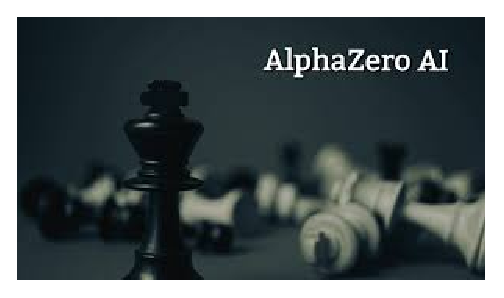
\includegraphics[width=0.5\textwidth]{Cap1/AlphaZero}
\caption{AlphaGo Zero, learning model that beat the best players of Go, Chess and Shogi, learning to play without previous human knowledge \cite{DBLP:journals/corr/abs-1712-01815}.}
\label{alphazero}
\end{figure}



\begin{figure}[ht!]
\centering
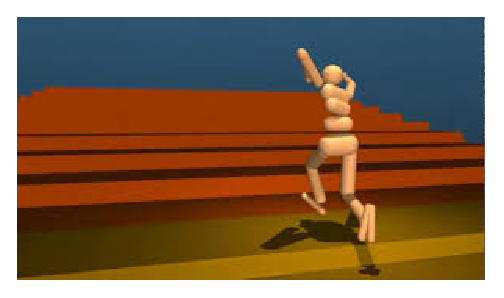
\includegraphics[width=0.5\textwidth]{Cap1/Locomotion}
\caption{Locomotion of Agent via Deep Reinforcement Learning \cite{DBLP:journals/corr/HeessTSLMWTEWER17}.}
\label{locomotion}
\end{figure}


\section{Contextualization}

RoboCup is an international scientific community aiming to advance the state of the art of intelligent robots. Its mission is that a team of robots will be able to beat the human team champion of the World Cup until the year 2050 \cite{10.1007/3-540-64473-3_46}. Since this is a goal with a range of different challenges to be solved, there are several categories of competition within the community.

In Robocup Soccer 3D Simulation League, as shown in Figure \ref{soccer3d}, there is a robot soccer competition in which each team has eleven Nao robots in a physical simulation environment called Simspark \cite{simspark2005}. The purpose in this case is to create and improve algorithms and physical models for the perception, locomotion, and strategy of the humanoid robot, before actually shipping them into hardware for real-world evaluation.

\begin{figure}[ht!]
\centering
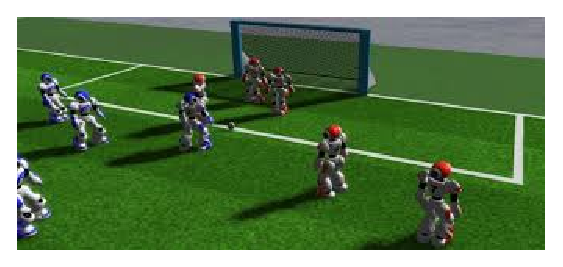
\includegraphics[width=0.5\textwidth]{Cap1/Soccer3D}
\caption{A Snapshot from the RoboCup Soccer 3D Simulation League.}
\label{soccer3d}
\end{figure}

Over the last few years, team efforts have been seen in three different areas, layers, or strands. The first area is considered more basic, meaning the construction of the agent that can model the environment and interact with it -- involving both the construction of a solid software architecture and the application of traditional techniques of localization and control of the humanoid robot \cite{AI1110-macalpine}.

The second layer, explored at the highest level, involves creating behaviors to perform actions within the game, given the modeled environment -- from the creation of models and heuristics for navigation to the creation of multiagent strategies for positioning and marking \cite{LNAI16-MacAlpine}.

The third strand, to be approached in this work, is the creation and optimization of models based upon learning for activities such as robot walking and kicking. Simulated categories have great value for learning test, mainly because they provide a benchmark for comparison and do not involve physical robots. Historically, teams with the best performance in these two issues are usually the best positioned within category competitions, due to the fact that they are able to maintain greater possession of the ball and are more offensive to the opposing goal.

\section{Objective}

Inspired from the context of the RoboCup 3D Simulation League and based upon some results from the recent techniques of Deep and Reinforcement Learning, this work aims to develop and evaluate some new learning models, based on Deep Reinforcement Learning, for the task of making a humanoid robot to kick the soccer ball inside the RoboCup Soccer 	3D Simulation environment.

\section{Scope}

In this work, Reinforcement Learning algorithms applied to models based upon Deep Neural Networks will be approached, in order to find, through gradient-based optimization techniques, optimal policies for kick control of the humanoid robot. These will be contrasted with classic control techniques coupled with evolutionary optimization strategies, widely used in the context of the RoboCup Soccer 3D Simulation League.

\section{Organization of this work}

This work is organized as follows: Chapter \ref{ch:soccer3d} will describe the RoboCup Soccer 3D Simulation League and the traditional methods used for the kick motion. Chapter \ref{ch:deeplearning} will cover the theory behind Deep Learning used in this work. Chapter \ref {ch:reinforcementlearning} will cover the theory behind Reinforcement Learning. Chapter \ref{ch:methodology} will explain all the methods and tooling used in experimentation. Chapter \ref{ch:results} describes the experimentation itself, detailing problem modeling, test scenarios, and the main results. Finally, Chapter \ref{ch:conclusion} will share some conclusions and suggestions for future work.



\chapter{Literature Review}\label{ch:soccer3d}
\section{The RoboCup Soccer3D Simulation League}
\subsection{Domain Description}
The RoboCup Soccer 3D Simulation League (Soccer 3D) is a particularly interesting challenge concerning humanoid robot soccer. It consists of a simulation environment for a soccer match with two teams, each one composed by up to 11 simulated Nao robots \cite{gouaillier2009}, the official robot used for the RoboCup Standard Platform League since 2008. The Soccer 3D is interesting for robotics research, since it involves high level multi-agent cooperative decision making, while providing a physically realistic environment, which requires control and signal processing techniques for robust low level skills.

The RoboCup 3D simulation environment is based on SimSpark \cite{simspark} , a generic
physical multi-agent system simulator. SimSpark uses the Open Dynamics Engine (ODE) library for its realistic simulation of rigid body dynamics with
collision detection and friction. The Nao robots has height of approximately 57 cm and 4.5 kilograms. The agent send torque commands to the simulator and receive perceptual data. Each robot has 22 joints with perceptors and effectors. Joints information are communication between agent and server, visual information and between agents happens in in the frequency of 50 Hz, 16.7 Hz and 25 Hz, respectively \cite{AAAI12-MacAlpine}. 

\subsection{ Kick Motion }
In the current level of the Soccer 3D evolution, motion control is a key factor in team's performance. Indeed, controlling a high degrees of freedom for a humanoid robot is acknowledged as one of the hardest problems in Robotics. Much effort has been devised to humanoid robot walking, where researchers have been very successful in designing control algorithms which reason about reduced order mathematical models based upon the Zero Moment Point (ZMP) concept, such as the linear inverted pendulum model \cite{kajita2001}. Nevertheless, these techniques restrict the robot to operate under a small region of its dynamics, where assumptions of the simplified models are still valid \cite{collins2005,muniz2016}.

Therefore, model-based techniques are hard to use for designing highly dynamic movements, such as long distance kicks and goalkeeper dives to defend goals from fast moving balls. In the robot soccer domain, a common approach for these movements is to employ keyframe movements, where motions are composed by sequences of robot postures. In this case, movements are designed off-line and executed in an open-loop fashion in execution time.

Due to the lack of mathematical models, an approach frequently employed is to rely on human intuition to design keyframe movements by hand, usually aided by graphical tools. However, this process is difficult, time consuming, and is often unable to obtain high performance motions given the high dimensionality of the search space. Other possible solution is to use motion to capture data from humans \cite{shon2005}, which has its own challenges due to the fact that the kinematic and dynamic properties of a humanoid robot differs greatly from those of a human.

\subsection{Keyframe Movements}

\begin{definition}
A \emph{keyframe} \( \mathrm{\mathbf{k}} = \left[ j_1, j_2, \dots, j_n \right]^T \in K \subseteq \mathbb{R}^n \) is an ordered set of joint angular positions, where \( K \) and \( n \) are the joint space and the number of degrees of freedom of the robot.
\end{definition}

\begin{definition}
A \emph{keyframe step} is an ordered pair \( \mathrm{\mathbf{s}} = \left( \mathrm{\mathbf{k}}, t \right) \in S = K \times \mathbb{R} \), where \( \mathrm{\mathbf{k}} \) is a keyframe and \( t \) is the time when the keyframe must be achieved with respect to the beginning of the movement. 
\end{definition}

\begin{definition}
A \emph{keyframe movement}, or simply a movement, is defined as \( \mathrm{\mathbf{m}} = \left( \mathrm{\mathbf{s}}_1, \mathrm{\mathbf{s}}_2, \dots, \mathrm{\mathbf{s}}_{\gamma}, r \right) \in M = S^{\gamma} \times \mathbb{R} \), where \( \gamma \) and \( r \) are the number of keyframe steps and the speed rate of the movement. In this representation, we assume the movement starts at time 0 and the first keyframe step represents the robot posture at the beginning of the movement. Therefore, \( t_1 = 0 \) and each time \( t_i, \forall i \geq 2 \) is a time since the beginning of the movement.
\end{definition}

Keyframe movements are executed in an open-loop fashion, where joint positions are computed through interpolation of keyframe steps based upon the current time. If the interface to the robot joints is not position-based, local controllers may be used to track the position references issued by the keyframe. For example, in the Simspark simulator, the simulated Nao Robot has speed-controlled joints, therefore, we use simple proportional controllers for each joint to track desired joint positions. To obtain smooth joint trajectories, we interpolate keyframe steps, by using cubic splines \cite{bartels1987}, which are functions of class \( \mathcal{C}^2 \). 

Finally, when a keyframe movement is requested, joint positions are often far away from movement's initial joint positions. Hence, by simply executing the keyframe movement in this case would result in high joints accelerations, which would probably make the robot to fall. To avoid this from happening, a transition movement based on linear interpolation is first employed to bring the joint positions to the initial joint positions required by the keyframe movement.

\subsection{Optimization Techniques}

In Soccer 3D environment, optimization techniques plays a important role to achieve competitive behaviors, because they are use to obtain faster and more robust motions.

Motion optimization means find the best values for each joint in the time instant during the whole motion. There's a lot of parameters involved, what turns manual tuning impossible. The common way to do this is modeling the motion and use optimization algorithms to find the best parameters for this model. For the kick motion, it means find the best keyframe and interpolator values. In the case of walking motion, we optimize the walk parameters, such as torso height, period and step size.

In the robotics simulation world, it's common to optimize using evolution strategies. \cite{tgmaximo} used Particle Swarm Optimization to optimize walk parameters. \cite{AAMAS11-urieli} compared the performance of several algorithms in Soccer3D context, such as Hill Climbing (HC), Cross-Entropy Method (CEM) \cite{Rubinstein:2004:CEM:1014902}, Genetic Algorithm and Covariance Matrix Adaptation Evolution Strategy (CMA-ES) \cite{cmaes}. The last one turns out to be the best for this kind of task and therefore is the most common in this environment. 

\begin{figure}[ht!]
	\centering
	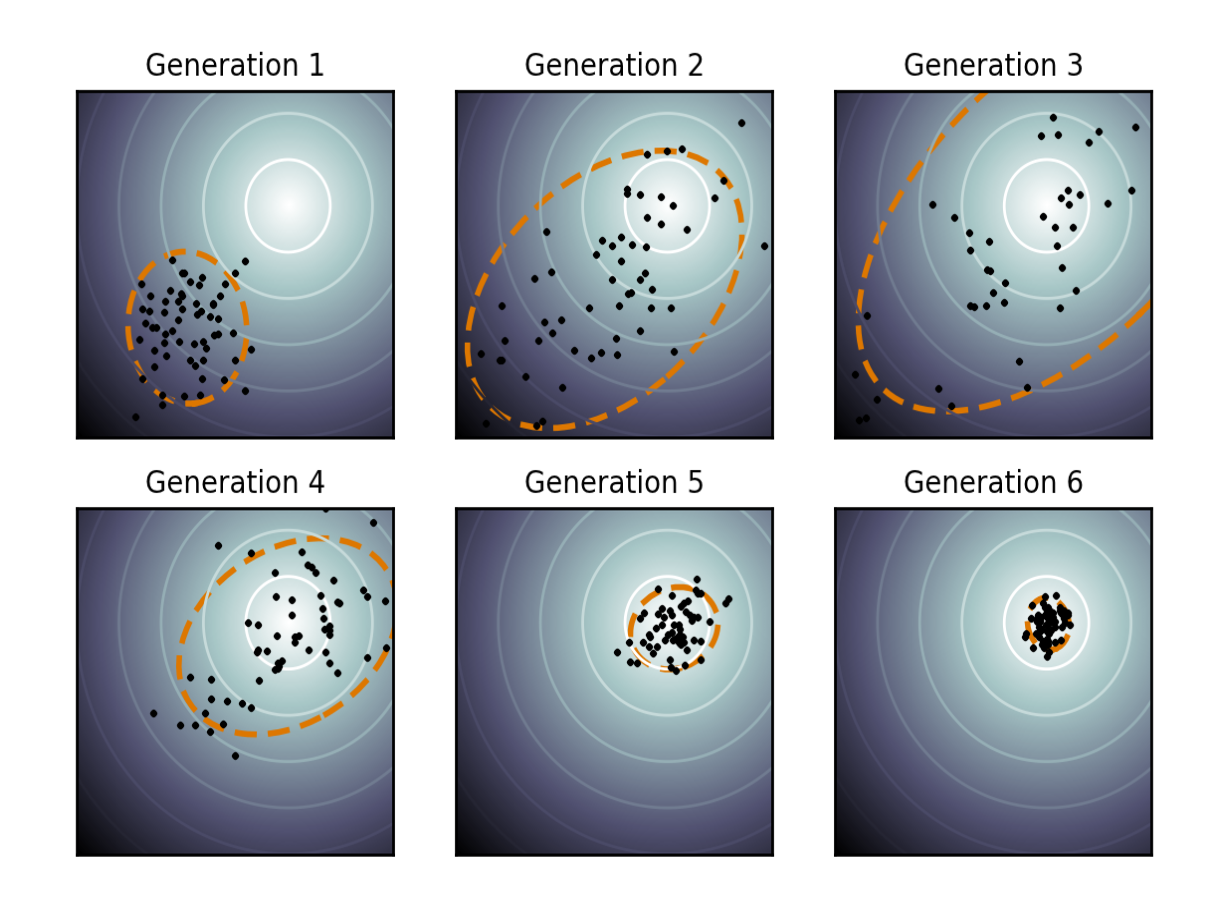
\includegraphics[width=0.8\textwidth]{Cap2/CMAES.eps}
	\caption{Illustration of an actual optimization run with covariance matrix adaptation on a simple two-dimensional problem
		\cite{cmaesfig}.}
	\label{cmaesfigure}
\end{figure}

The CMA-ES algorithm is a policy search algorithm that generates a population of parameter sets -- also known as "candidates" -- sampled from a multivariate Gaussian distribution. These sets are evaluated with respect of a fitness measure. When all the candidates in group are evaluated, the mean of the multivariate Gaussian
distribution is recalculated as a weighted average of the
candidates with the highest fitnesses. The covariance matrix
of the distribution is also updated to bias the generation
of the next set of candidates toward directions of previously
successful search steps \cite{AAMAS11-urieli}, as shown in Figure \ref{cmaesfigure}. Even the algorithm works well for kick and walk motions, it doesn't scale well for hundreds or thousands of parameters \cite{mcalpine2017}.


\section{Reinforcement Learning for Control}

In this work, we will use more recent techniques that are able to optimize in this scale using policy gradient based algorithm instead of evolution strategies. These algorithms are based on Reinforcement Learning theory applied for control tasks.

Classic reinforcement learning algorithms are called tabular solution methods and uses dynamic programming for map state to actions. The most famous algorithms are Monte-Carlo methods, Temporal-Difference learning, SARSA \cite{Rummery94on-lineq-learning} and Q-Learning \cite{Watkins:1989}. These algorithms are good to solve toy problems, such as grid worlds and multi-armed bandits. However, they don't scale well for problems with greater state space.

However, these methods were improved using the idea of function approximation instead of tabular solutions. The new algorithms started to use other learning representations, since linear combination of features until neural networks. The last one was a huge improvement in the Reinforcement Learning field. With the arise of Deep Q-Networks (Figure \ref{dqn}), we were able to surpass human-level performance in several Atari games, as show in \cite{mnih2015humanlevel}.

\begin{figure}[ht!]
	\centering
	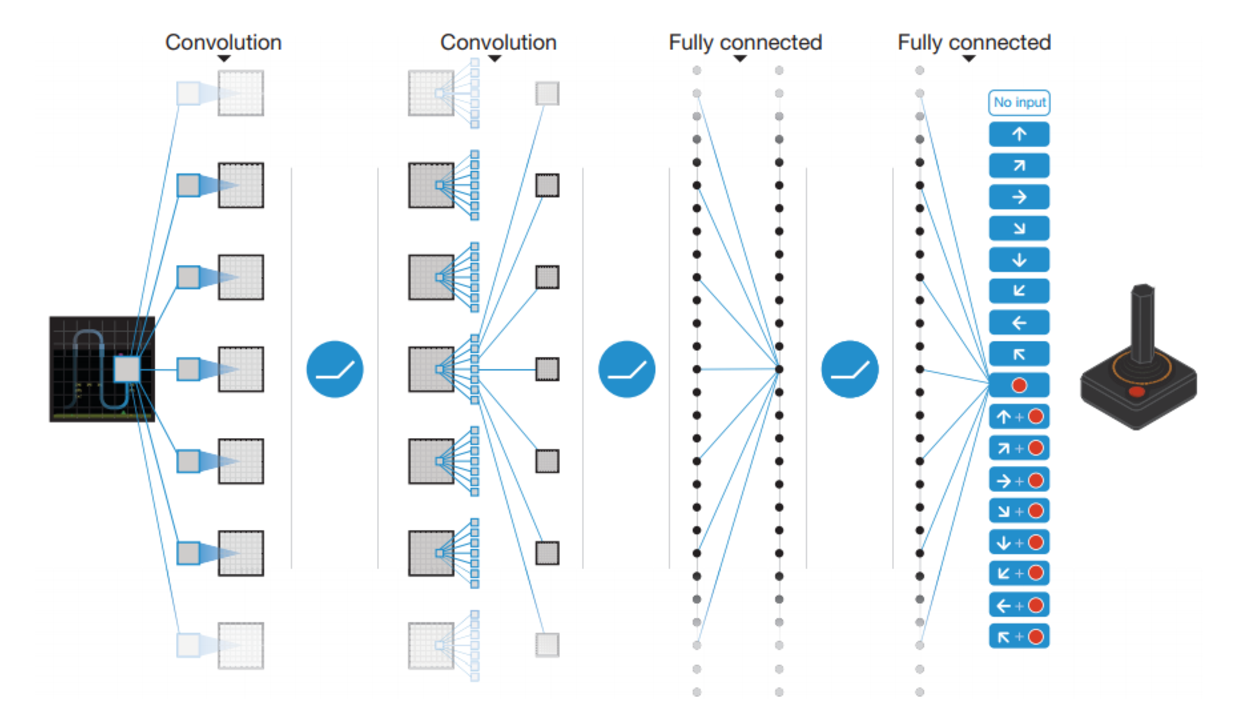
\includegraphics[width=0.8\textwidth]{Cap2/dqn.eps}
	\caption{Human level control through deep reinforcement learning in atari games
		\cite{mnih2015humanlevel}.}
	\label{dqn}
\end{figure}

With the arise of Deep Learning and its new techniques and the development of new computer architectures such as GPUs and TPUs, reinforcement learning has been able to scale as well, surpassing top players from the best table games. For example, the AlphaGo \cite{alphago} won from the human top player of Go, considered the hardest tabular game. It used a Monte-Carlo Tree Search with a Deep Neural Network to find a optimal policy through self-play and without any human knowledge. The evolution of AlphaGo, called AlphaZero \cite{alphazero} was able to learn not just Go, but also Chess and Shogi within a couple of hours.

On the other side, all the tasks mentioned before are discrete control. The problem of kick motion is related to continuous control. In this kind of problem, there's no discrete actions, but a interval of them. Therefore, the algorithms are different and must satisfact new optimization challenges.

In the last years, several algorithms arised in order to improve the performance in control tasks. These algorithms are commonly applied to MuJoCo environment \cite{mujoco}, the most famous benchmark for continuous control tasks. Among such methods, we highlight A2C \cite{a2c}, ACER \cite{acer}, DDPG \cite{ddpg}, GAIL \cite{gail}, HER \cite{her}, TRPO \cite{trpo} and PPO \cite{ppoalgorithm}. The TRPO and PPO algorithms will be covered in deep later, and the last one will be used in the learning framework proposed in this work, since it has proved to perform better in MuJoCo benchmark.

In terms of applications, \cite{DBLP:journals/corr/HeessTSLMWTEWER17} applied a distributed variation of PPO in MuJoCo and were able to learn parkour movements and run without in a model free way. These motions, however, are weird, asymmetric and, sometimes, unstable. \cite{peng2018} applied the same algorithm but with key modifications in the reward function and optimization process, resulting in better and more human motions.

The most recent and impressive application of PPO was in OpenAI Five \cite{openaifive}. It consists in five independent neural networks that form a team to play the online game Dota 2. This team was trained in the equivalent of 180 years of continuous self-play, using 256 GPUs and 128 thousand of CPUs, and won from the $99.95^{th}$ percentile human player team in a restricted environment. This is impressive not just because the environment is challenging -- due to the partial observability, long time horizon and high-dimensional, continuous spaces -- but also because of the multi-agent strategy layer learned. The network architecture used by OpenAI Five is shown in Figure \ref{openaifive}.

\begin{figure}[ht!]
	\centering
	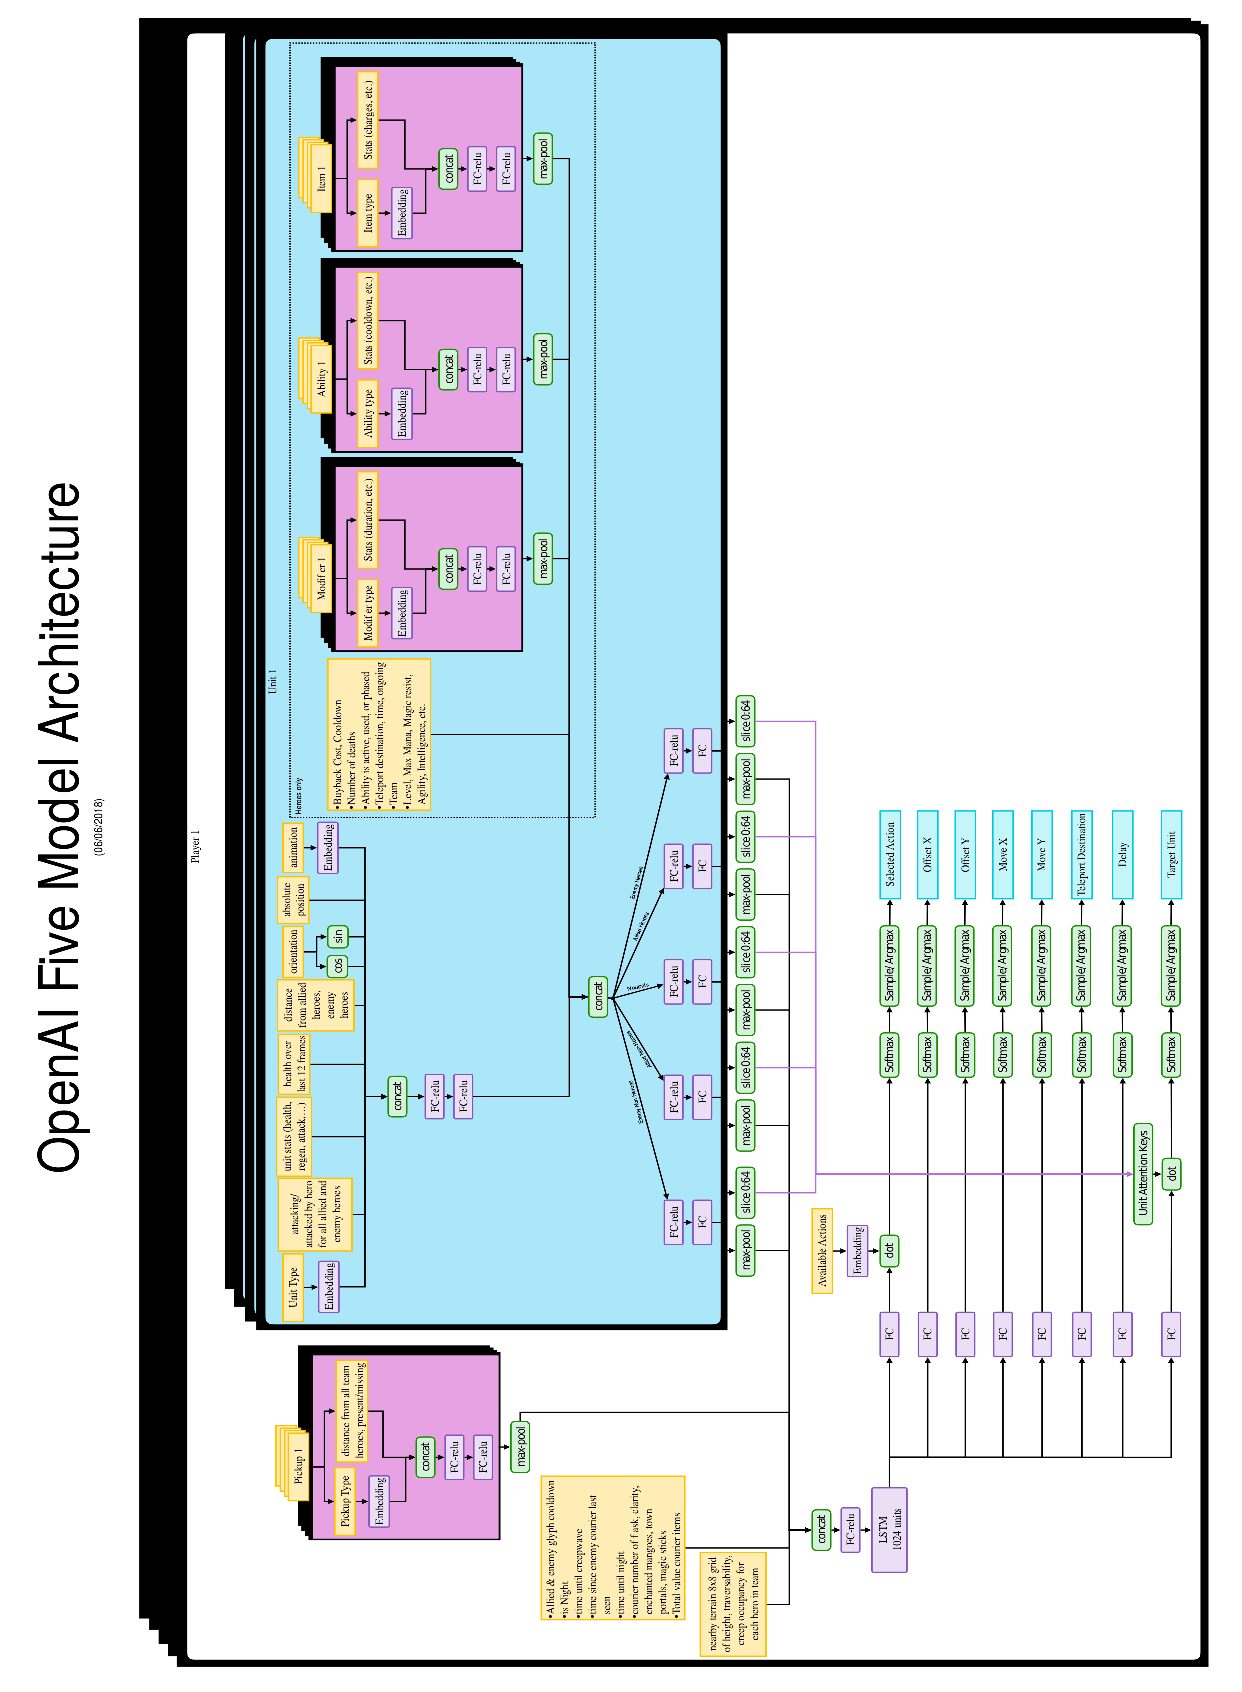
\includegraphics[angle=270, scale=0.5]{Cap2/openaifive.eps}
	\caption{OpenAI Five network architecture \cite{openaifive}.}
	\label{openaifive}
\end{figure}



\chapter{Deep Learning}\label{ch:deeplearning}
\section{Neural Networks}
\label{sec:neural_networks}
Neural Networks are a learning representation which the goal is to approximate some function \( f^* \). Data collected from an environment encodes an underlying function \( \mathrm{\mathbf{y}} = f^*(\mathrm{\mathbf{x}}) \) that maps an input \( \textbf{x} \) to an output \( \mathrm{\mathbf{y}} \), which may be a category from a classifier or a continue value in regression problems. The neural network defines an approximate mapping \( \mathrm{\mathbf{y}} = f(\mathrm{\mathbf{x}};\boldsymbol{\theta}) \), by learning the values of the parameters \(\boldsymbol{\theta}\), which result in the best function approximation. Figure \ref{fig:ann} shows a neural network and an artificial neuron in detail.

\begin{figure}[!htbp]
\centering
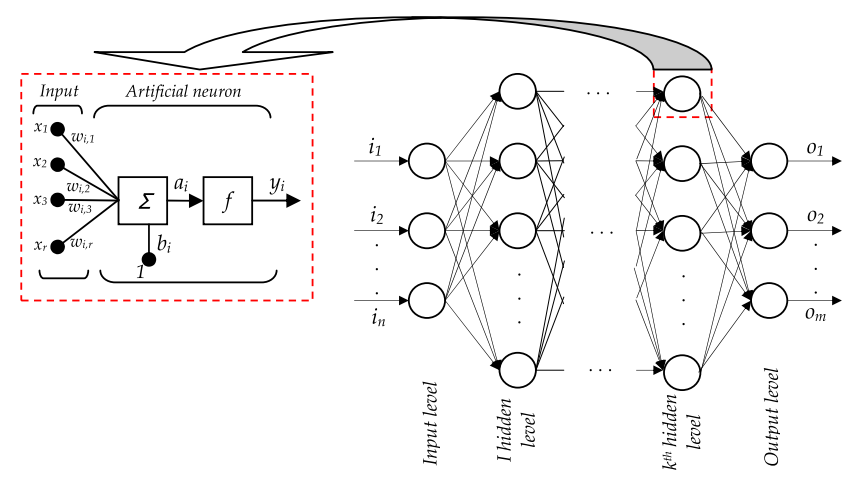
\includegraphics[width=0.8\textwidth]{Cap3/ann}
\caption{An artificial neuron within a feed forward artificial neural network \cite{dejan12}. }
\label{fig:ann}
\end{figure}

These networks are typically represented by composing together many different functions, which are associated with a directed acyclic graph, by describing a computational model. For example, we might have three layers (each of them representing a function \( f^{(1)}, f^{(2)} \), and \(f^{(3)} \)), connecting in a chain and resulting in a final representation \( f(\mathrm{\mathbf{x}}) = f^{(3)}(  f^{(2)} ( f^{(1)}(\mathrm{\mathbf{x}}))) \).

During a neural network training, the objective is to adjust \(f(\mathrm{\mathbf{x}})\) to match \(f^{*}(\mathrm{\mathbf{x}})\), by using the training dataset, which provides noisy examples of \(f^{*}(\mathrm{\mathbf{x}})\) evaluated in different points. The training examples directly specify what the output layer must do at each point \(\mathrm{\mathbf{x}}\), but the learning algorithm must decide how to use all layers to produce this desired output \cite{Goodfellow-et-al-2016}.

\subsection{A Neuron}\label{sec:neuron}

The idea of a neural network starts in the concept of a neuron. Figure \ref{fig:neurondetail} illustrates it in detail.

\begin{figure}[!htbp]
	\centering
	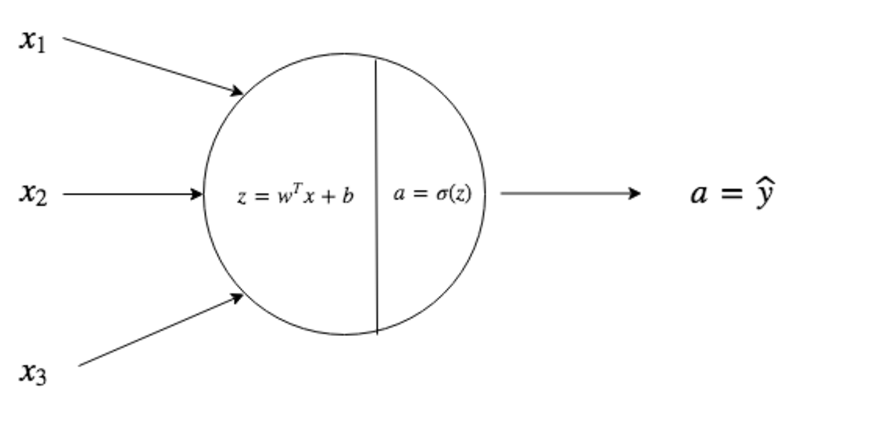
\includegraphics[width=0.8\textwidth]{Cap3/neurondetail.eps}
	\caption{An artificial neuron in detail.}
	\label{fig:neurondetail}
\end{figure}

In a neuron, the first operation is the product between inputs and the respective weights, which represents how much each input signal will influence the computation of that neuron. The core idea of a neural network is calculate the value of those weights in order to generate a better representation of the data generator distribution.

To this linear combination, it's added a bias value, which purpose is to add the capacity of neuron representation by translation, due to the fact this value doesn't rely on the inputs. Figure \ref{fig:bias} shows how weights and bias affect the function representation, described by equation \ref{eq:neuronequation}.


\begin{equation}
z = w^{T}x + b
\label{eq:neuronequation}
\end{equation}



\begin{figure}[!htbp]
	\centering
	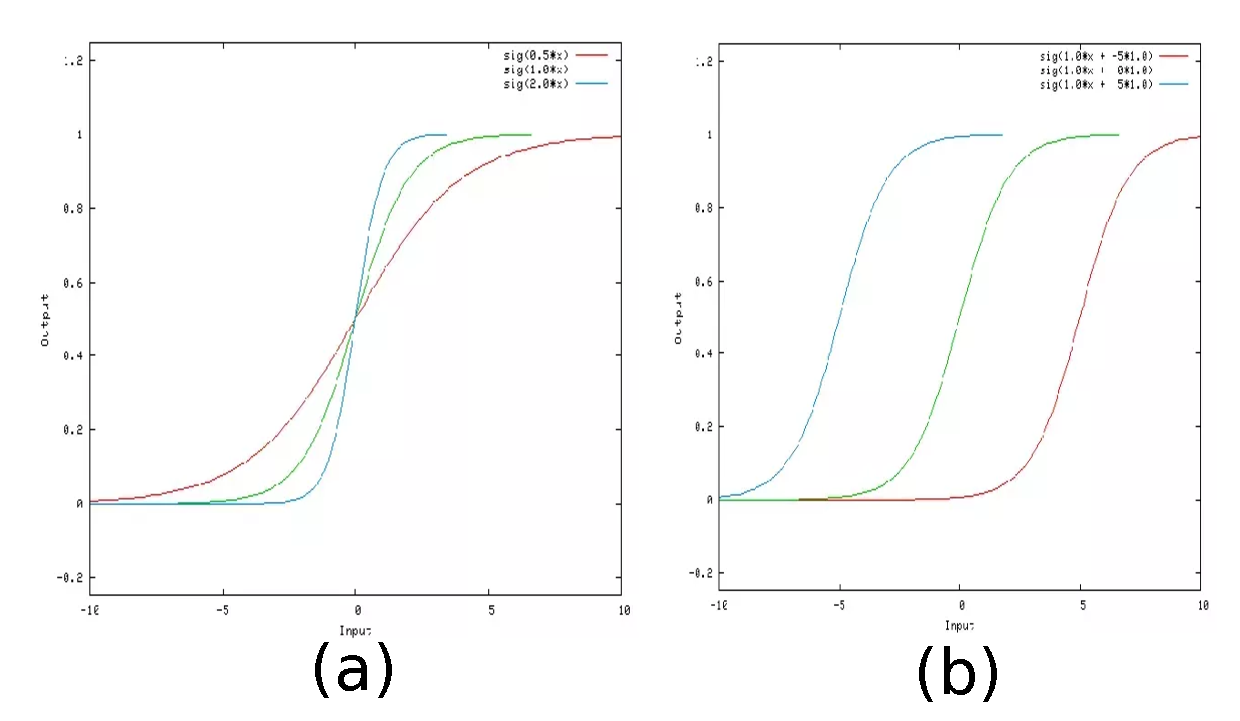
\includegraphics[width=0.9\textwidth]{Cap3/bias.eps}
	\caption{Function representation: in (a), we have a sigmoid function where weights vary. In (b), the same sigmoid but only bias varies.}
	\label{fig:bias}
\end{figure}

The final operation from a neural is the activation function computed using the linear combination as input. In the context of neural networks, this is a non-linear function whose purpose is add the neuron's capacity of representation. Without this idea, the network would be only able to learn linear functions, which will result in poor representation of complex data distributions. Equation \ref{eq:neuronactivation} shows the neuron activation. These functions will be described deeper in section \ref{sec:activationfunction}.

\begin{equation}
a = \sigma({z})
\label{eq:neuronactivation}
\end{equation}


\subsection{Neural Network Representation}

A neural network is a combination of neurons in several layers. It's basically a directed acyclic graph (DAG) where each node performs the operations described in subsection \ref{sec:neuron}. Figure \ref{fig:neuralnetworkrepresentation} shows the representation of a neuron.

\begin{figure}[!htbp]
	\centering
	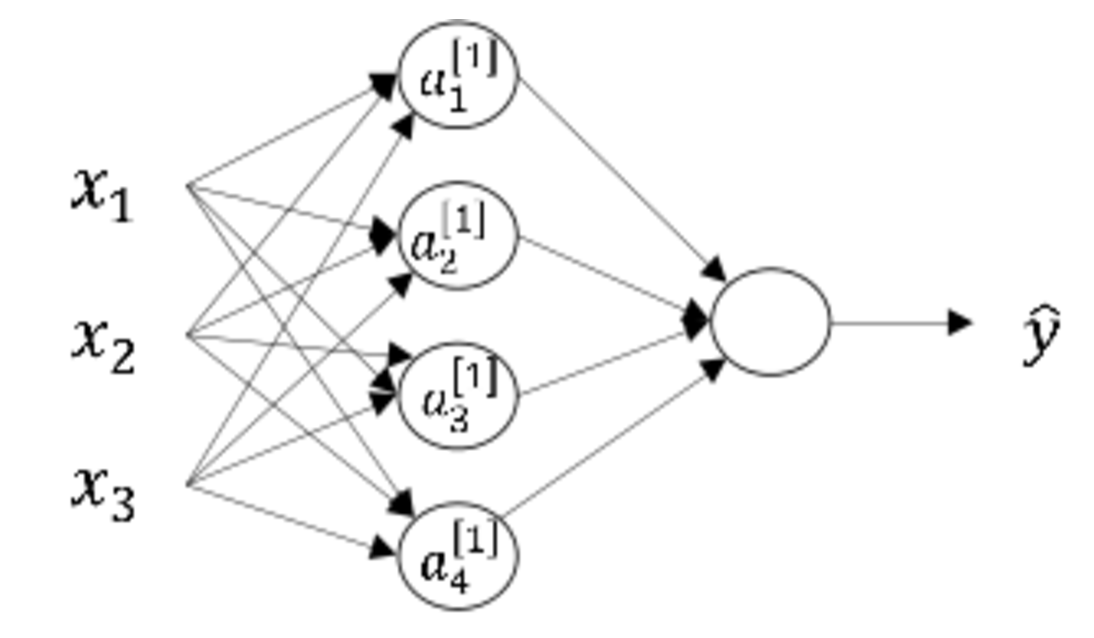
\includegraphics[width=0.7\textwidth]{Cap3/neuralnetworkrepresentation.eps}
	\caption{Neural Network representation.}
	\label{fig:neuralnetworkrepresentation}
\end{figure}

It is worth to mention the math notation used in this work. The neuron $a^{j}_{i}$ represents the $i^{th}$ neuron in the $j^{th}$ layer of network.

The flow of a input tensor in a neural network occurs in the following manner: first, neurons from the same layer performs its calculations. Then, the output of them will serve as input of the next layer. This sequence will keep going until reach the output layer. Equations \ref{eq:nn_begin} to \ref{eq:nn_final} represent the flow from Figure \ref{fig:neuralnetworkrepresentation}.


\begin{align}\label{eq:nn_begin}
z^{[1]} = W^{[1]}x + b^{[1]}\\
a^{[1]} = \sigma(z^{[1]})\\
z^{[2]} = W^{[2]}a^{[1]} + b^{[2]}\\
a^{[2]} = \sigma(z^{[2]})
\label{eq:nn_final}
\end{align}

$W^{i}$ and $b^{i}$ are defined, respectively, as:

\begin{align}
W^{[i]} = \begin{bmatrix}
w^{T[i]}_1 & w^{T[i]}_2 & \dots & w^{T[i]}_n
\end{bmatrix} \\
b^{[i]} = \begin{bmatrix}
b^{[i]}_1 & b^{[i]}_2 & \dots & b^{[i]}_n
\end{bmatrix}
\end{align}

In general, we can represent a layer $i$ recursively as:

\begin{align}
z^{[i]} = W^{[i]}a^{[i-1]} + b^{[i]}\\
a^{[i]} = \sigma(z^{[i]})
\end{align}


The first layer of a neural network is called \textbf{input layer} and represents its inputs. The last layer is the \textbf{output later} and represents its outputs. All layers between those are \textbf{hidden layers}. The greater is the number of layers, the deeper the network is.

\subsection{Vectorization}\label{sec:vectorization}

Vectorization is a technique where a network calculates the output of several examples in a batch at the same time, instead of calculate them sequentially. Basically, we consider as input:

\begin{align}
X = \begin{bmatrix}
x^{T}_1 & x^{T}_2 & \dots & x^{T}_n
\end{bmatrix}
\end{align}

Therefore, the network layers' equations change to:

\begin{align}
Z^{[i]} = W^{[i]}A^{[i-1]} + b^{[i]}\\
A^{[i]} = \sigma(Z^{[i]})
\end{align}

Using vectorized implementations the network can explore better Single Instruction Multiple Data (SIMD) architectures and then speedup learning.

\section{Activation Functions}\label{sec:activationfunction}
As described in subsection \ref{sec:neuron}, an activation function uses the linear combination as input to give a non-linear representation and the improve network learning capacity. Without this, it only is able to represent linear functions.

There are several activation functions. We will describe the most common used in deep learning research.

\subsection{Logistic Sigmoid}

Equation \ref{eq:sigmoid} shows the logistic sigmoid function.

\begin{equation}
\sigma(z) = \frac{1}{1 + e^{-z}}
\label{eq:sigmoid}
\end{equation}

This function is commonly used to produce the parameter of a Bernoulli distribution because its range is (0,1). Furthermore, it saturates when its argument is very positive or very negative, meaning the function becomes very flat and insensitive to small changes in its input \cite{Goodfellow-et-al-2016}. Figure \ref{fig:sigmoid} illustrates the logistic sigmoid function.

\begin{figure}[!htbp]
	\centering
	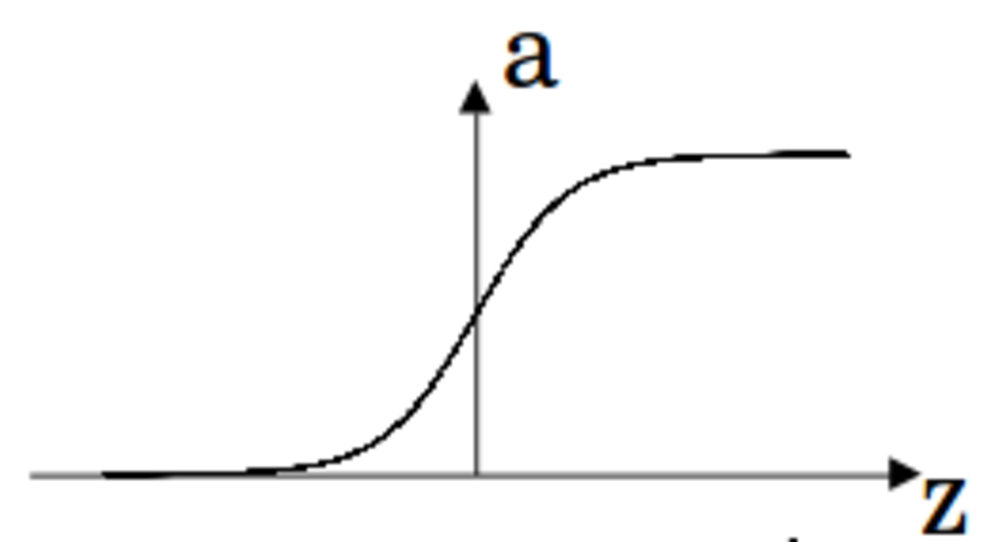
\includegraphics[width=0.7\textwidth]{Cap3/sigmoid.eps}
	\caption{Illustration of Sigmoid function.}
	\label{fig:sigmoid}
\end{figure}

\subsection{Hyperbolic Tangent}

Equation \ref{eq:tanh} shows hyperbolic tangent ($tanh$).


\begin{equation}
tanh(z) = \frac{e^{z} - e^{-z}}{e^{z} + e^{-z}}
\label{eq:tanh}
\end{equation}

It is close related to logistic function, because:

\begin{equation}
tanh(z) = 2\sigma(2z) - 1
\label{eq:tanhsigmoid}
\end{equation}

Hyperbolic tangent is considered a sigmoidal activation function as well, but typically performs better than sigmoid. It resembles the identity function more closely due to its symmetry in $x$ axis. Train a neural network with this activation function resembles a linear model when the input can be kept small, which makes training easier.

Figure \ref{fig:tanh} illustrates hyperbolic tangent.

\begin{figure}[!htbp]
	\centering
	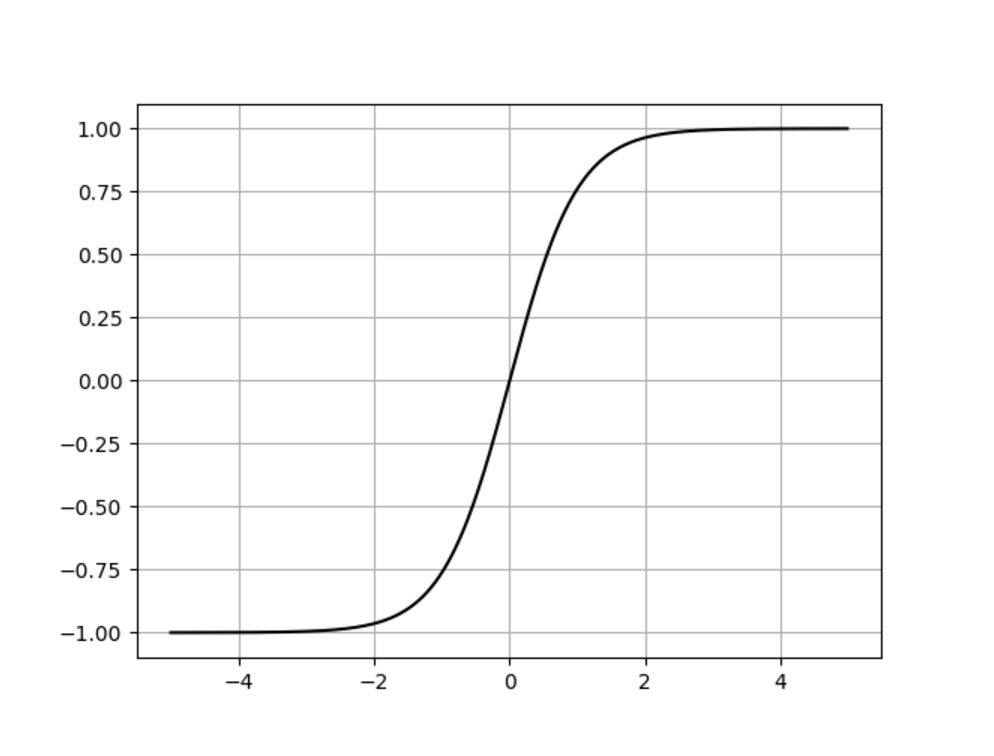
\includegraphics[width=0.7\textwidth]{Cap3/tanh.eps}
	\caption{Illustration of $tanh$ function.}
	\label{fig:tanh}
\end{figure}


\subsection{Rectified Linear Unit - ReLU}

Rectified Linear Unit is a activation function very similar with a linear unit. It is described by equation \ref{eq:relu}:

\begin{equation}
g(z) = max(0,z)
\label{eq:relu}
\end{equation}

The only difference between a linear unit and a rectified linear unit is
that a rectified linear unit outputs zero across half its domain. This makes the
derivatives through a rectified linear unit remain large whenever the unit is active.
The gradients are not only large but also consistent. The second derivative of the
rectifying operation is 0 almost everywhere, and the derivative of the rectifying
operation is 1 everywhere that the unit is active. This means that the gradient
direction is far more useful for learning than it would be with activation functions
that introduce second-order effects \cite{Goodfellow-et-al-2016}. Figure \ref{fig:relu} illustrates this activation function.

\begin{figure}[!htbp]
	\centering
	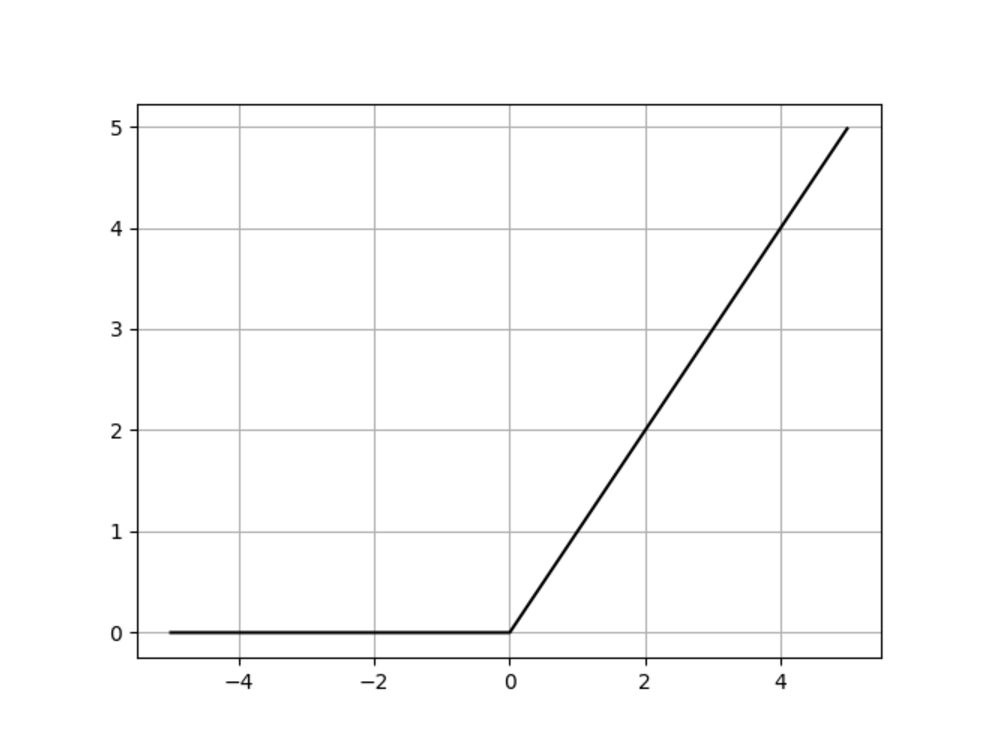
\includegraphics[width=0.7\textwidth]{Cap3/relu.eps}
	\caption{Illustration of ReLU function.}
	\label{fig:relu}
\end{figure}

\cite{glorot2011a} motivate rectified linear units from
biological considerations. The half-rectifying nonlinearity was intended to capture
these properties of biological neurons: 
\begin{itemize}
\item For some inputs, biological neurons are
completely inactive. 
\item For some inputs, a biological neuron’s output is proportional
to its input. 
\item Most of the time, biological neurons operate in the regime where
they are inactive (i.e., they should have sparse activations).
\end{itemize}

\subsection{Leaky ReLU}

One drawback to rectified linear units is that they cannot learn via gradient-based methods on examples for which their activation is zero. Leaky ReLU \cite{leakyrelu} is a
generalization of rectified linear units guarantee that they receive gradient everywhere.

Equation \ref{eq:leakyrelu} represents the Leaky ReLU activation.


\begin{equation}
g(z) = max(\alpha z,z) 
\text{, where } \alpha \in (0,1)
\label{eq:leakyrelu}
\end{equation}

Rectified linear units and all generalizations of them are based on the
principle that models are easier to optimize if their behavior is closer to linear. Figure \ref{fig:leakyrelu} illustrates this activation function.


\begin{figure}[!htbp]
	\centering
	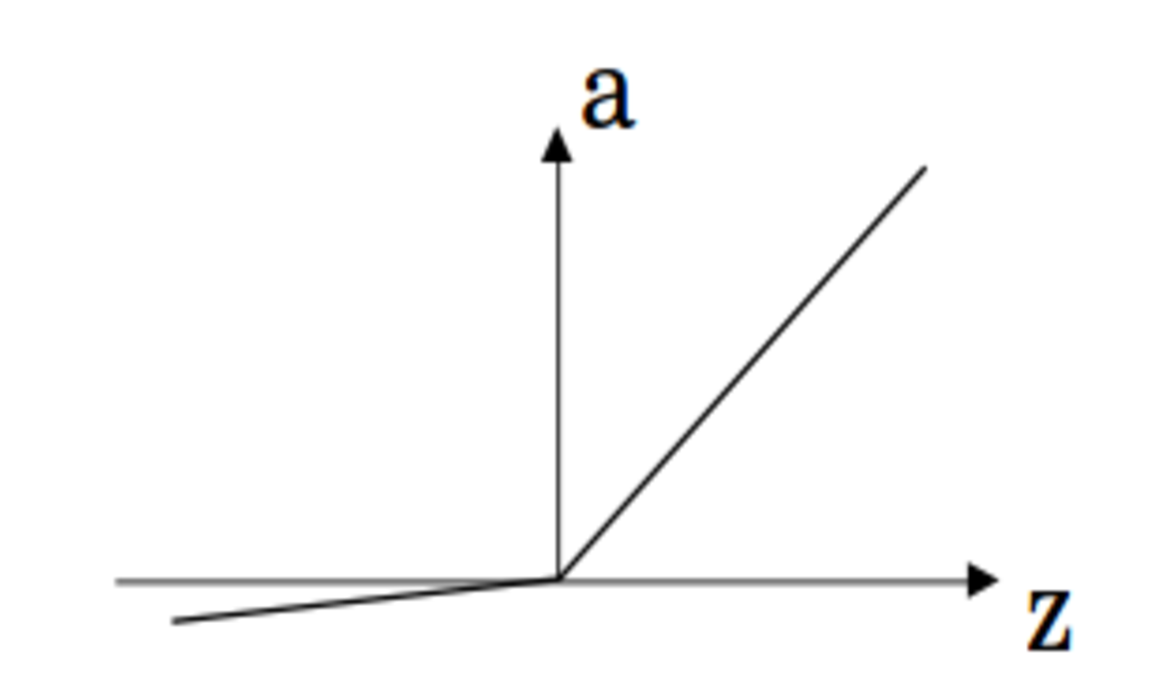
\includegraphics[width=0.7\textwidth]{Cap3/leakyrelu.eps}
	\caption{Illustration of leaky ReLU function.}
	\label{fig:leakyrelu}
\end{figure}


\section{Cost Function}

In the context of neural networks, gradient-based algorithms are broadly used, especially those based on the backpropagation idea \cite{hinton88}. The purpose of these algorithms are to propagate the gradient of a cost function through the whole network, in order to minimize the cost function. Most modern neural networks perform this optimization strategy, by using maximum likelihood, i.e. the cross-entropy between the training data and the model distribution:

\begin{equation}
J(\boldsymbol{\theta}) = -\mathbb{E}_{\mathrm{\mathbf{x}},\mathrm{\mathbf{y}}\sim \hat{p}_{data}}\log{p_{model}(\mathrm{\mathbf{y}} | \mathrm{\mathbf{x}})}
\label{eq:cost_function_ml}
\end{equation}

In this work, we used the mean squared error loss function, in order to fit data distributions. Indeed, we may show that both cost functions are closely related. Let us consider normally distributed errors:

\begin{equation}
{p_{model}(\bvec{y} | \bvec{x})} = \mathcal{N}( \bvec{y}; f (\bvec{x}; \boldsymbol{\theta}), \sigma^{2}\bvec{I})
\label{eq:errors}
\end{equation}
where \(f (\bvec{x}; \boldsymbol{\theta})\) and \(\sigma^{2}\bvec{I}\)  are the mean and covariance of this distribution. By substituting Eq. \eqref{eq:errors} in Eq. \eqref{eq:cost_function_ml}:

\begin{equation}
J(\boldsymbol{\theta}) = \frac{1}{2}\mathbb{E}_{\bvec{x},\bvec{y}\sim \hat{p}_{data}} \lVert \bvec{y} - f (\bvec{x}; \boldsymbol{\theta}) \rVert ^{2} + const
\label{eq:cost_function_expectation}
\end{equation} 

The constant term does not depend on \( \boldsymbol{\theta} \) and may be dropped. By explicitly evaluating the expectation in Eq. \eqref{eq:cost_function_expectation}, we arrive at the mean squared error cost function:

\begin{equation}
J(\boldsymbol{\theta}) = \frac{1}{2m} \sum^{m}_{i} \lVert y_{i} - f (\bvec{x}; \boldsymbol{\theta}) \rVert ^{2}
\end{equation}

It can be shown that maximum likelihood estimator is the best estimator asymptotically, when the number of samples $m$ tends to infinity, in terms of its rates of convergence as $m$ increases. Furthermore, this estimator has the property of consistency, under certain conditions that must be satisfied by the data distribution, and efficiency, in terms of achieve lower generalization errors.	

\section{Gradient Descent}\label{gradientdescent}

The objective of a neural network training is find the parameters $W$ and $b$ that approximates the function represented by itself and the data generator distribution, by minimizing the cost function established. In math terms, it means:

\begin{equation}
(W^{*},b^{*}) = \argmin_{W,b}J(W, b, x)
\end{equation}


The Gradient Descent technique is a iterative method that calculates the derivative of the loss function and applies them as learning updates according to a learning rate factor, $\alpha$, previously set. Figure \ref{fig:gradientdescent} illustrates the application of this technique in the context of two variables.

\begin{figure}[!htbp]
	\centering
	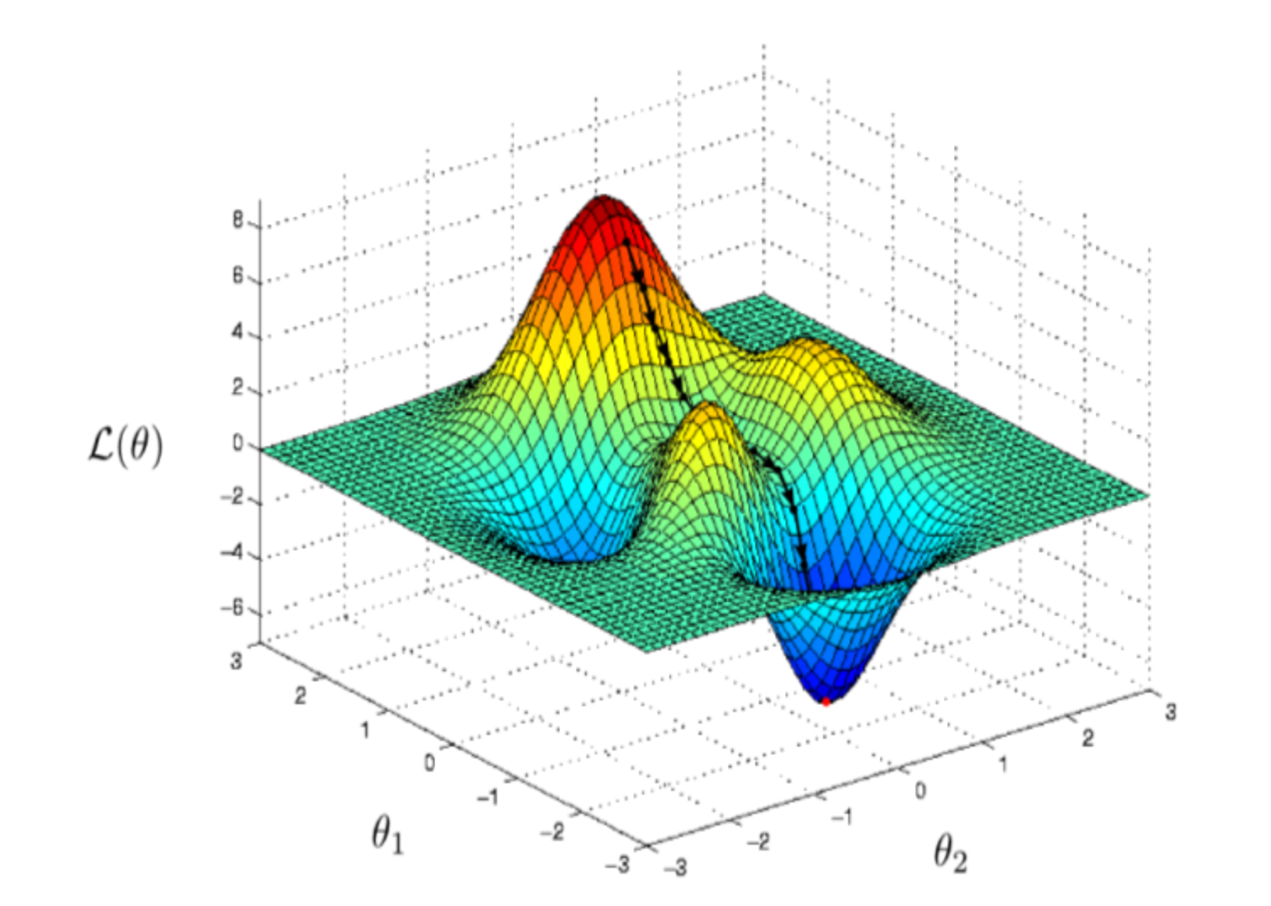
\includegraphics[width=0.7\textwidth]{Cap3/gradientdescent.eps}
	\caption{Illustration of gradient descent in a two variables optimization
	\cite{tgilharco}.
	}
	\label{fig:gradientdescent}
\end{figure}


As an example, given the following cost function (where $m$ is the number of samples, $\hat{y}$ is the prediction of the network and $y$ is the ground-truth):

\begin{equation}
J(W,b) = \frac{1}{m}\sum^{n}_{i = 1}\mathcal{L}(\hat{y}, y)
\end{equation}


The gradient with respect of the parameters $W$ and $b$ can be given by:

\begin{align}
\frac{\partial{J(W,b)}}{\partial{W}} = \frac{1}{m}\sum^{n}_{i = 1}\frac{\partial{\mathcal{L}(\hat{y}, y)}}{\partial{W}}\\
\frac{\partial{J(W,b)}}{\partial{b}} = \frac{1}{m}\sum^{n}_{i = 1}\frac{\partial{\mathcal{L}(\hat{y}, y)}}{\partial{b}}
\end{align}

After these calculations, we are able to apply these gradients using the learning update rule:


\begin{align}
W = W - \alpha\frac{\partial{J(W,b)}}{\partial{W}}\\
b = b - \alpha\frac{\partial{J(W,b)}}{\partial{b}}
\end{align}

These steps are applied iteratively until the function converges to a optimal value. It's important to mention that there are no guarantees the optimization will converge to a global optima, i.e, it is possible to get stuck in local optima. However, in practical applications, this is not a huge problem.

\section{Backpropagation}
In the case described in section \ref{gradientdescent} we computed the gradient directly with respect to parameters $W$ and $b$. However, in neural networks, we have to compute the gradients that correspond to all and layers and not just to the output layer. For this, we need to use the chain rule of calculus.

Let $x$ be a real number, and let $f$ and $g$ both be functions mapping from a real
number to a real number. Suppose that $y = g(x)$ and $z = f (g(x)) = f (y)$. Then
the chain rule states that


\begin{equation}
\frac{dz}{dx} = \frac{dz}{dy}\frac{dy}{dx}
\end{equation}

We can generalizes to vectorial case. Suppose that $\boldsymbol{x} \in \mathbb{R}^{m} , \boldsymbol{y} \in \mathbb{R}^{n}$, $g$ maps from $\mathbb{R}^{m}$ to $\mathbb{R}^{n}$ , and $f$ maps from $\mathbb{R}^{m}$ to $\mathbb{R}^{n}$. If $\boldsymbol{y} = g(\boldsymbol{x})$ and $\boldsymbol{z} = f( \boldsymbol{y})$, then

\begin{equation}
\frac{\partial{z}}{\partial{x_i}} = \sum_{j} \frac{\partial{z}}{\partial{y_{j}}}\frac{\partial{y_{j}}}{\partial{x_{i}}}
\end{equation}
 
It can be generalized more generic in a way that can be applied to tensors:

\begin{equation}
\nabla_{\textbf{X}}z = \sum_{j}(\nabla_\textbf{X}Y_{j})  \frac{\partial{z}}{\partial{Y_{j}}}
\label{eq:backprop}
\end{equation}

The backpropagation takes equation \ref{eq:backprop} recursively, until the gradient is propagated to all layers of the neural network. Algorithm \ref{alg:backprop} \cite{Goodfellow-et-al-2016} shows in a simple way how to apply backpropagation to a deep neural network.

\begin{algorithm}[!htbp]
	\caption{Backward computation for a deep neural network}
	\begin{algorithmic} 
		\STATE After the forward computation, compute the gradient on the output layer:
		\STATE $\boldsymbol{g} \leftarrow \nabla_{\boldsymbol{\hat{y}}}J = \nabla_{\boldsymbol{\hat{y}}}\mathcal{L}(\boldsymbol{\hat{y}},y)$
		\STATE \textbf{for} $k = l, l - 1,
		 \dots, 1$ \textbf{do}
		
		\STATE \hspace{5mm} Convert the gradient on the layer’s output into a gradient into the pre-nonlinearity activation (element-wise multiplication if f is element-wise):
		\STATE \hspace{5mm} $\boldsymbol{g} \leftarrow \nabla_{\boldsymbol{a^{(k)}}}J = \boldsymbol{g} \odot f'(\boldsymbol{a}^{(k)})$
		\STATE \hspace{5mm} Compute gradients on weights and biases:
		\STATE \hspace{5mm} $\nabla_{\boldsymbol{b}^{(k)}}J = \boldsymbol{g}$
		\STATE \hspace{5mm} $\nabla_{\boldsymbol{W}^{(k)}}J = \boldsymbol{g} \boldsymbol{h}^{(k-1)T}$
		\STATE \hspace{5mm} Propagate the gradients w.r.t. the next lower-level hidden layer’s activations:		
		\STATE \hspace{5mm} $\boldsymbol{g} \leftarrow \nabla_{\boldsymbol{h}^{(k - 1)}}J = \boldsymbol{W}^{(k)T}\boldsymbol{g}$
		\STATE \textbf{end for}
	\end{algorithmic}
	\label{alg:backprop}
\end{algorithm}

\section{Optimization Algorithms}
In Deep Learning community, gradient-based optimization is well established. However, in state-of-art research the backpropagation idea had several improvements to make learning better. In this section, we will explore some of these improvements and present the optimizer used in experimentation.

\subsection{Batch, Mini-batch and Stochastic Gradient Descent}
There are ways to use the data in order to apply learning updates. Accordingly to section \ref{sec:vectorization}, using vectorization makes possible to calculate several losses at the same time. However, sometimes the dataset is very large in a way it is costly to apply a single batch several times. On the other side, apply updates using one sample at a time can result in a biased gradient and also can be costly due to the fact we need to apply an update for each sample. Therefore, the batch size can change a lot the learning process.

The Batch Gradient Descent calculates the cost function for each sample in the dataset and only updates the model after all samples have been evaluated. In this way, there are fewer updates and the gradient is more precise, due to the fact we consider several samples to regularize it. So, the training and convergence are more stable. However, this variation of gradient descent can result in local optima convergence and turns to be very slow with large datasets.

The Stochastic Gradient Descent calculates the cost function and updates the model for each samples in dataset. Using this variation, there are more frequent updates which can give feedback about the model fast and result in faster learning to some problems. Furthermore, the noisy update allows exploration in function optimization, avoiding local optima (Figure \ref{fig:batchvsstochastic}). However, there is a high computational cost of applying updates so frequently and the same noise can make hard for the last optimization steps. Equation \ref{eq:sgd} shows the learning update rule for Stochastic Gradient Descent:

\begin{equation}
W = W - \alpha\frac{\partial{J(W,b, x^{(i)})}}{\partial{W}}
\label{eq:sgd}
\end{equation}

\begin{figure}[!htbp]
	\centering
	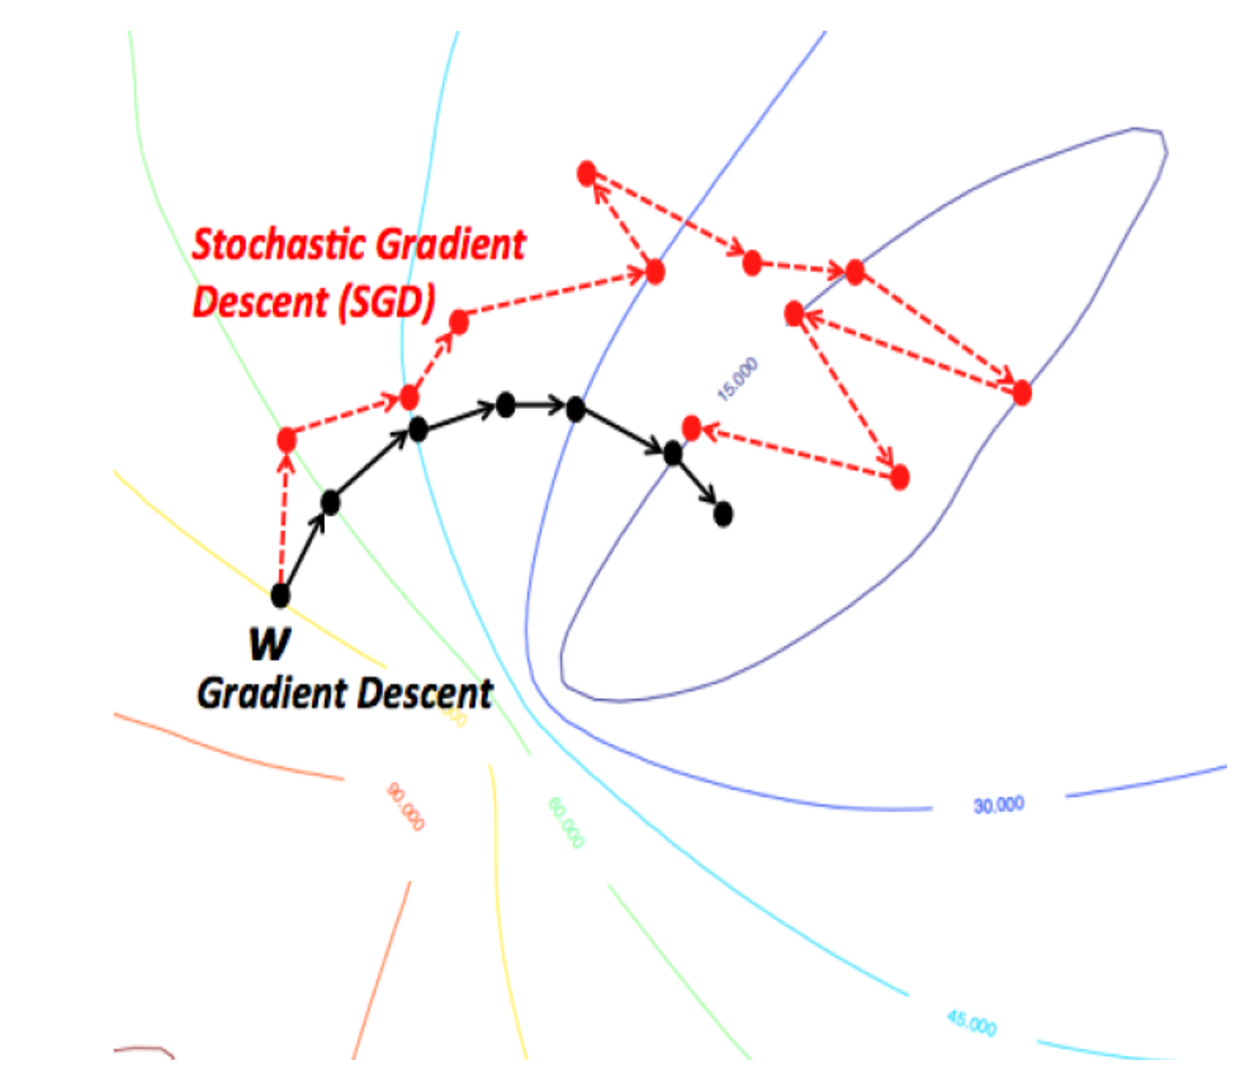
\includegraphics[width=0.8\textwidth]{Cap3/batchvsstochastic.eps}
	\caption{Illustration of 	Stochastic Gradient Descent optimization.
	}
	\label{fig:batchvsstochastic}
\end{figure}


Figure \ref{fig:lossfunctiongdvariants} shows how cost function commonly behaves in each variation of Gradient Descent described.

\begin{figure}[!htbp]
	\centering
	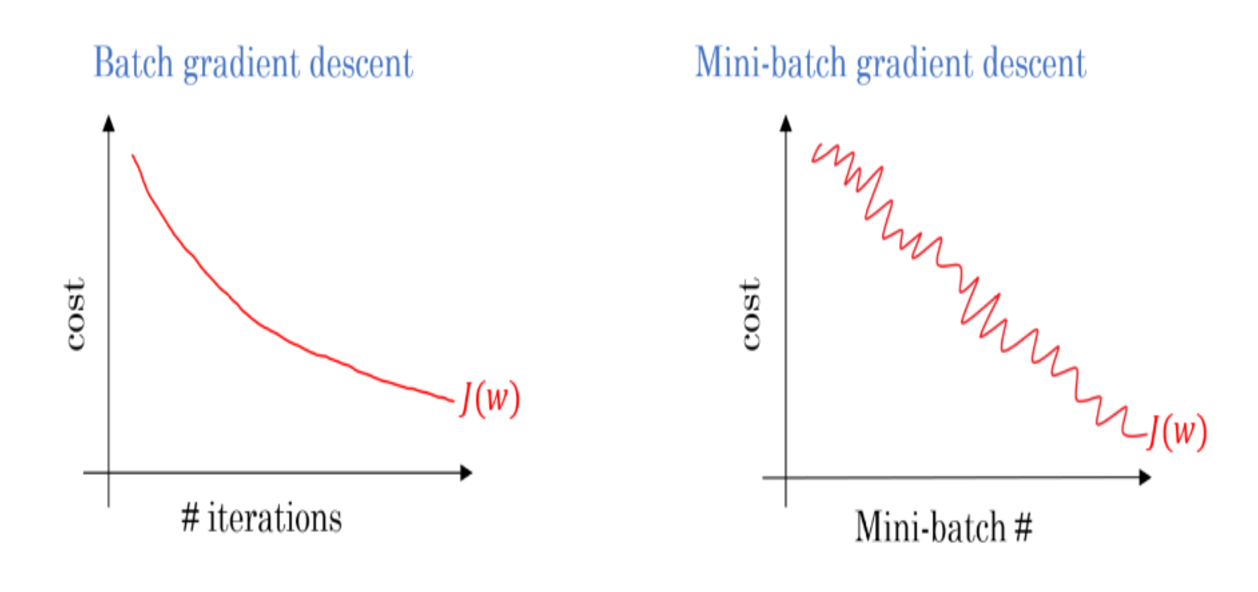
\includegraphics[width=0.8\textwidth]{Cap3/lossfunctiongdvariants.eps}
	\caption{Illustration of how each variation of Gradient Descent commonly behaves.
	\cite{dabbura2017}.
	}
	\label{fig:lossfunctiongdvariants}
\end{figure}



There is a third variant. The Mini-batch Gradient Descent is something in between batch and stochastic variants, where the algorithm splits dataset into small batches and each of them will apply learning updates. This version seeks to find a balance between the robustness of SGD and the efficiency of BGD. It is the most common implementation used in Deep Learning \cite{brownlee2017}. However, the downside of this variation is the fact we need to set a new hyperparameter and tune it manually.



\subsection{Momentum}

Momentum is a technique for accelerating gradient descent that accumulates a velocity vector in directions of persistent reduction in the objective across iterations \cite{Sutskever:2013:IIM:3042817.3043064}. It uses the idea of exponentially weighted moving averages, accumulating gradients for each mini-batch accordingly to a hyperparameter $\beta$. This term will manage how much the last gradient will affect in the final velocity, following Equations \ref{eq:momentum} and \ref{eq:momentum_b}. Momentum aims primarily to solve two problems: poor conditioning of the
Hessian matrix and variance in the stochastic gradient \cite{Goodfellow-et-al-2016}.


\begin{align}\label{eq:momentum}
v_{dW} = \beta v_{dW} + (1 - \beta)dW\\
v_{db} = \beta v_{db} + (1 - \beta)db
\label{eq:momentum_b}
\end{align}

Where $dW$ and $db$ are, respectively:

\begin{align}
dW = \frac{\partial{J(W,b)}}{\partial{W}}\\
db = \frac{\partial{J(W,b)}}{\partial{b}}
\end{align}

Therefore, using Momentum, the learning update is:

\begin{align}\label{eq:momentumupdate}
W = W - \alpha v_{dW}\\
b = b - \alpha v_{db}
\end{align}

The intuition behind Momentum is to filter the gradient, "reinforcing" it in the effective directions and removing the noisy ones. Then, it makes harder to apply learning updates in the wrong direction caused by noise samples. Figure \ref{fig:momentum} shows how Momentum changes Gradient Descent updates.


\begin{figure}[!htbp]
	\centering
	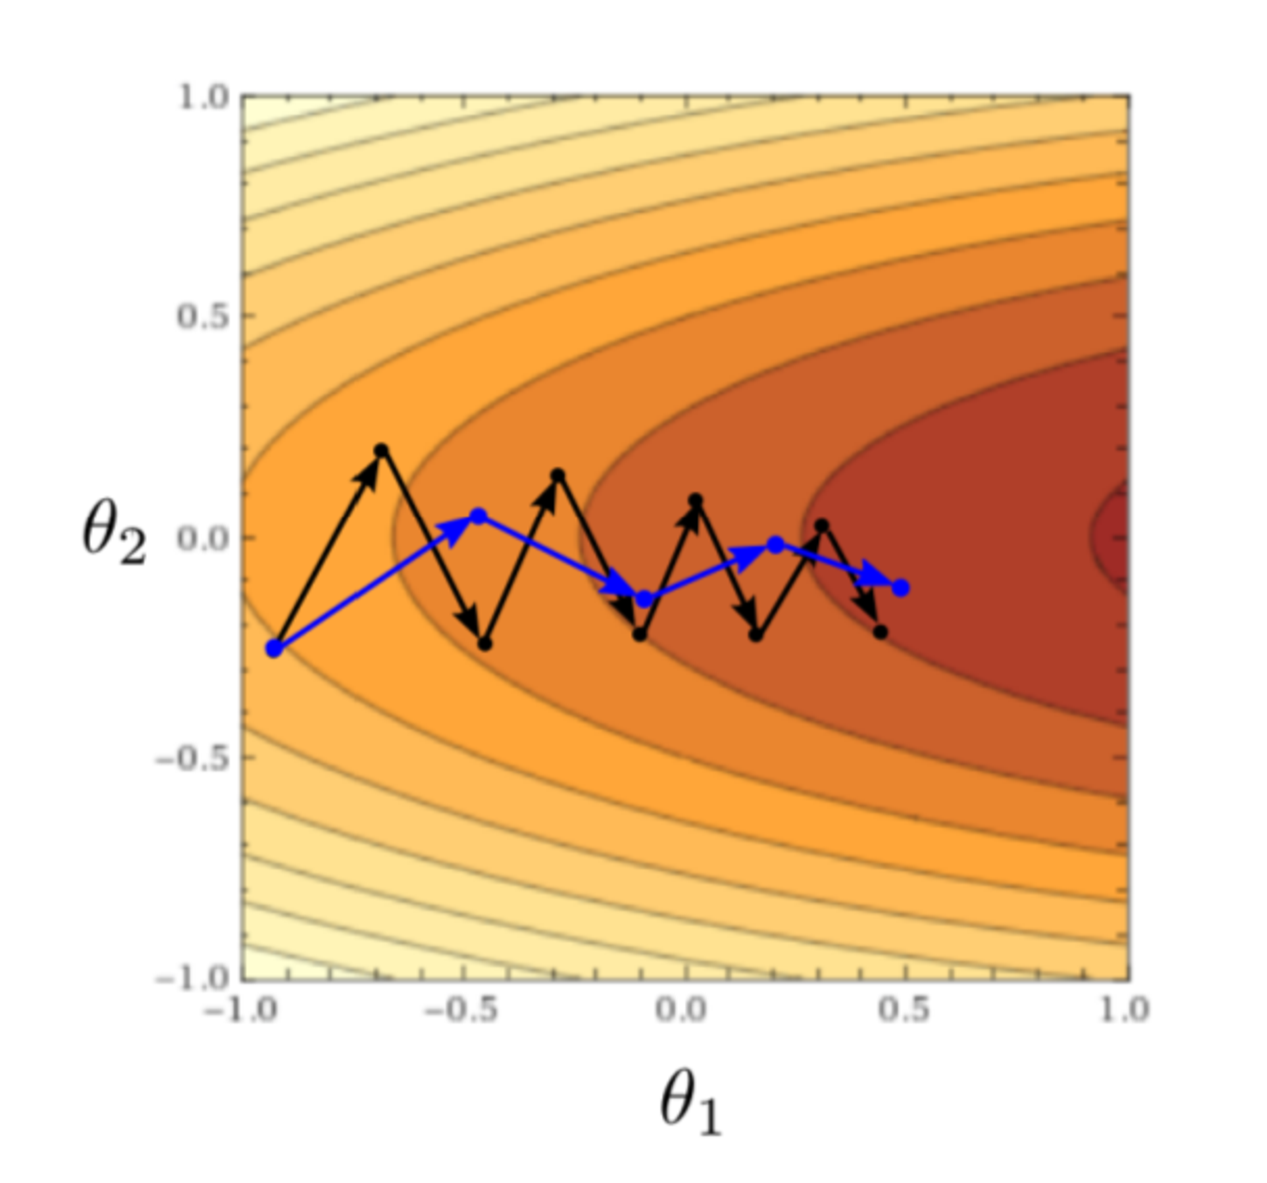
\includegraphics[width=0.8\textwidth]{Cap3/momentum.eps}
	\caption{ Illustration of how Gradient Descent with Momentum (blue arrows) and without it (black arrows)
		\cite{tgilharco}.
	}
	\label{fig:momentum}
\end{figure}

\subsection{RMSProp}

RMSProp \cite{hinton2012} uses the idea of exponentially weighted moving average for gradient accumulation in a non-convex optimization scenario. Instead of using the gradient to update velocity as Momentum does, RMSProp uses the square of this gradient, as shown in Equations \ref{eq:rmsprop} and \ref{eq:rmsprop_b}.


\begin{align}\label{eq:rmsprop}
v_{dW} = \beta v_{dW} + (1 - \beta)dW^2\\
v_{db} = \beta v_{db} + (1 - \beta)db^2
\label{eq:rmsprop_b}
\end{align}

\subsection{Adam}

\section{Random Initialization}
\subsection{Xavier Initialization}

\section{Learning Rate Decay}

Utilizando um valor fixo de , n ao h a garantias da convergencia do
algoritmo, que em geral ocorre para valores grandes de . A figura 3.19 ilustra um caso
onde o algoritmo diverge para uma fun c ao de uma u
ica vari vel. Existem alternativas
que garantem a convergencia do algoritmo (embora frequentemente acompanhadas de um
1
aprendizado mais lento), sendo uma das mais populares  = na t- esima itera c ao.


\chapter{Methodology}\label{ch:methodology}
\section{The Kick Motion Problem}

First of all, we need to understand why kick motion is a hard task for learning models, which justifies the usage of scalable techniques such as Deep Reinforcement Learning.

\begin{itemize}
	\item \textbf{Long Time Horizons}: The simulation server runs 50 cycles per second. Each action has minor impact individually, but can collapse the motion in future. Furthermore, the final objective is inject velocity in the ball and it happens only after the whole motion. So, the real reward is very delayed.
	
	\item \textbf{Partially-observed state}: The agent doesn't have full information from the environment and perception data is noisy. Therefore, all information used in training is liable to have errors that can make learning harder.
	
	\item \textbf{High-dimensional, continuous action space}: In the kick motion, at each timestep, the agent have to act in each of 22 joints. Each joint can assume any possible angle. If we consider the agent could assume only two possible actions for each joint, then it has $2^{22} = 4.194.304$ possible combinations of actions. Just to compare: the average number of actions in chess is 35; in Go, 250.
\end{itemize}
\section{Experimentation Setup}\label{sec:experimentation_setup}
In order to find the best method for learn the Kick Motion, we tested several techniques to compare them and find out that one which converges faster and results in the better and more robust kick. In the next subsections, we will describe each of the methods evaluated in this work.

\subsection{Hybrid Learning Model -- HLM}
In the Hybrid Learning Model (HLM), the training process occurs in two phases. The first one, a supervised learning phase, we learn the keyframe used by using a neural network, reproducing almost the same motion that we already had previously. The intuition behind this is if the agent starts from a good initial point in the optimization problem, it could be easier to get better results applying the gradient in the neighborhood of that point. The reward starts with a good value and the starting motion is well defined. Otherwise, if the optimization starts in a random point, it could be impossible to reach a good motion and probably the agent will get stuck in a local optima. This idea is shown in Figure \ref{optimization_intuition}.

\begin{figure}[!htbp]
	\centering
	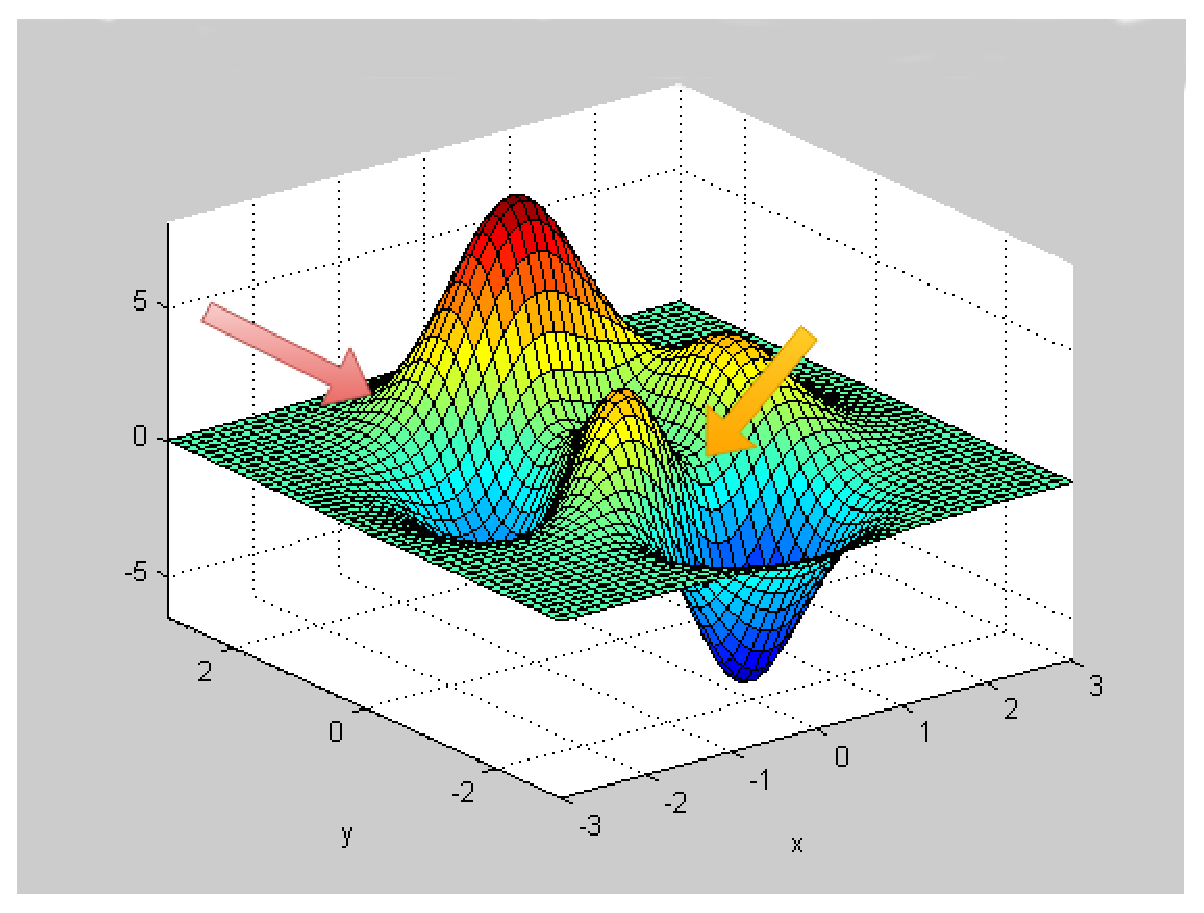
\includegraphics[width=0.5\textwidth]{Cap5/optimization_final.eps}
	\caption{In the hybrid model, we can ensure the starting point is near of the optimal solution (orange arrow); otherwise, the starting point can be bad and harder to optimize (red arrow).}
	\label{optimization_intuition}
\end{figure}

\subsection{Reinforcement with Naive Reward - RNR }
In this learning model, we just use reinforcement learning with a simple and directly reward. As our task is related to kick the ball, the "naive" reward is composed by its velocities after the kick motion, as shown in \ref{naive_reward}, where $s$, $v$ and $u$ are actual state, the vector of velocity and weight parameters, respectively. We call it naive because we don't pass to the learning model any idea of how the motion have to be performed - just what we expect to have as final objective. 

It is important to highlight that the techniques described could be used jointly as building blocks of a more labored model.

\begin{equation}
R(s) = u^{T}v
\label{naive_reward}
\end{equation}

\subsection{Reinforcement with Reference Reward - RRR }
In this learning model we add a term that compares the actual performance with a reference motion, as shown in \ref{complete_reward}:

\begin{equation}
R(s) = w_{ref}^{T}r
\label{complete_reward}
\end{equation}

In this equation, $w_{ref}$ are weight parameters for each joint and $r$ is the absolute value of the difference between joint values in that state and the reference (equation \ref{diffjoints}).

\begin{equation}
r(\theta, \theta_{0}) = \lVert\theta - \theta_{0}\rVert
\label{diffjoints}
\end{equation}

The intuition behind this weight parameters is because we have some joints more important than others. For example, some joints from the leg that kicks the ball themselves could collapse the whole motion if the error is high. On the other hand, joints from the neck are not so important to the kick. Therefore, it's natural to penalize differently in each case.

Lastly, the reference motion used was the keyframe kick previously mentioned and also used in HLM.


\subsection{Reinforcement with Initial State Distribution - RISD}\label{risd}

The Initial State Distribution is a technique related to where the episode starts to collect data to use in the learning. Without this technique, all episodes start in the beginning of the motion. However, the problem of this strategy is because the policy is forced to learn the motion in a sequential manner, first learning the early phases of the motion, and then incrementally progressing towards the later phases. This can be problematic for the kick motion. Another disadvantage of a fixed initial state is the resulting exploration challenge. The policy only receives reward retrospectively, once it has visited a state. Therefore, until a high-reward state has been visited, the policy has no way of learning that this state is favorable \cite{peng2018}.

To implement Initial State Distribution, we used a uniformly random variable that could assume any value in the set of states from the reference motion previously described. Suppose we pick the value $s$. Then, we start the episode running reference motion, from its first state until $s$. Finally, we start to collect data and perform the actions from the running policy.

\subsection{Reinforcement with Early Termination - RET}

The Early Termination technique is related to where the episode ends. Without early termination, all motions stops in the same state, which means that the episode length is fixed. The problem of this is because if the motion fails somehow during its execution, all the data collected after the failure will harm learning and evaluation of later stages.

In the kick motion task, the early termination will be triggered when the robot falls during the motion. This behavior will ensure two things: first, that we don't collect wrong data, as mentioned before; and second, to gain more reward and have longer episodes, the agent will be forced to learn a kick motion that doesn't fall -- which will be very good in game situation.



\section{Supervised Learning Setup}\label{supervised_learning_setup}
\subsection{The Dataset}\label{AA}
In order to use supervised learning for learning keyframe motions using neural networks in the HLM model, we first need to construct a dataset. A dataset consists of samples of keyframe steps. Samples were collected within the Soccer 3D environment with a frequency of 50 Hz. We acquired these samples in two different ways.

In the first one, we commanded an agent of our team to execute specific motions and sampled the reference joint positions computed by our code. In this case, we sampled the kick and get up keyframe motions \cite{muniz2016}. Notice that, for this approach to be successful, one needs access to the source-code.

The second approach involved changing the Soccer 3D server source-code to provide current joint positions of a given robot, in a similar way as described in \cite{macalpine2013}. This allowed us to acquire motion datasets from other teams, without any knowledge of how these movements are implemented. In this case, we collected two types of kicks based on keyframes and sampled joint values of the walking engine \cite{AAAI12-MacAlpine}.


\subsection{Neural Network Architecture and Hyperparameters}

The neural network has to be able to learn how to interpolate between samples, which actually happens. The architecture that performed best -- in terms of mean absolute error minimization and simplicity -- is shown in Figure ~\ref{fig:model_plot}. A deep neural network with 2 hidden, fully connected layers of 75 and 50 neurons was used. The output layer has 23 regression neurons, which represent the 22 joint angles and a neuron which output indicates if the motion has ended or not. The neurons in each hidden layer use the LeakyReLU activation function \cite{leakyrelu}: 

\[
  f(x) = \left\{
     \begin{array}{@{}l@{\thinspace}l}
       \alpha x,   & \quad x < 0  \\
       x, & \quad x \ge0 \\
     \end{array}
   \right.
\]
where $\alpha$ is a small constant. This activation function was used to improve the representation capacity of the neural network, adding support for non-linear functions.

\begin{figure}[!htbp]
\centering
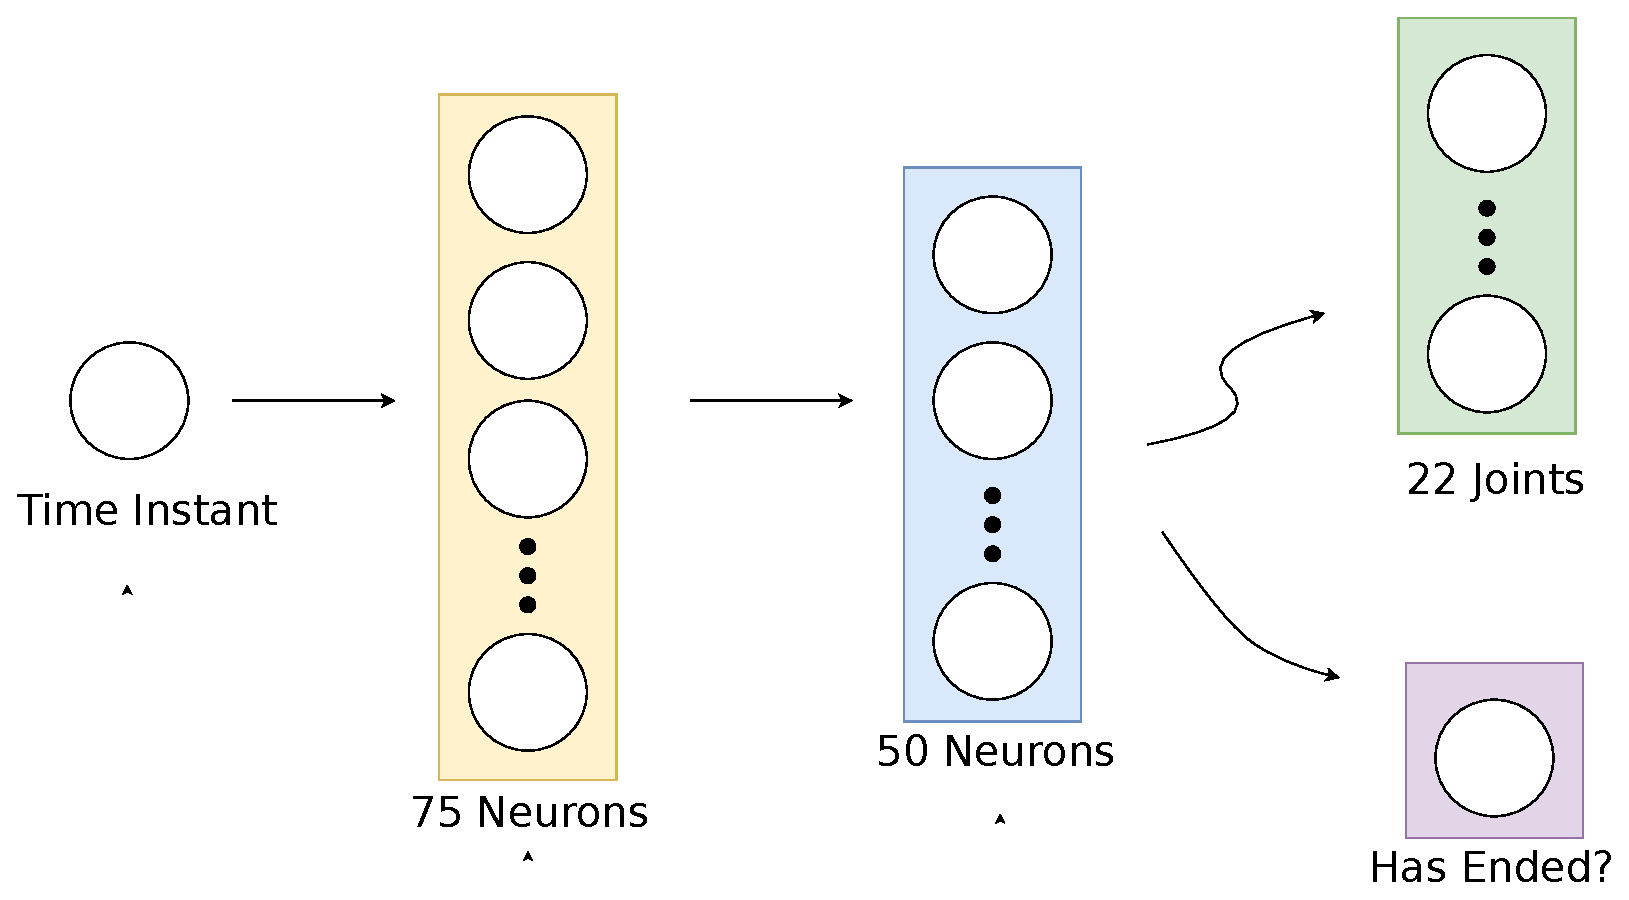
\includegraphics[width=0.5\textwidth]{Cap5/architecture}
\caption{The architecture of a neural network designed to learn motions.}
\label{fig:model_plot}
\end{figure}

This architecture resulted in thousand of parameters to optimize, as exposed in Table \ref{tab:network_summary}. A very high number, when compared to more traditional optimization approaches \cite{AAAI12-MacAlpine}. Notice that, by increasing the number of parameters usually allows representing better movements.

\begin{table}[htbp]
\caption{The Network Summary}
\begin{center}
\begin{tabular}{|c|c|c|c|}
\hline
\textbf{Layer}&{\textbf{Neurons}}& \textbf{Activation}& \textbf{Parameters} \\
\hline
Dense & 75 & LeakyReLU & 150  \\
\hline
Dense & 50 & LeakyReLU & 3800 \\
\hline
Dense & 23 & Linear & 1173 \\
\hline
\end{tabular}
\begin{tabular}{|c|c|}
\hline
\textbf{Total Parameters} & 5123 \\
\hline
\end{tabular}
\label{tab:network_summary}
\end{center}
\end{table}


\subsection{The Training Procedure}
Since keyframe motions are executed in an open-loop fashion, the sequence of joint positions are always the same for different repetitions, independently of robot's state. Therefore, by adding samples of multiple executions of the same motion would not make our dataset richer. So, we decided to use only one repetition for each movement for faster training. In the case of the walking motion, we collected samples within one walking period.

During the training, we used 50 thousands epochs divided into 5 training phases, where the learning rate was decreased between phases, in order to achieve better performance. First, we executed 30000 epochs, by using the learning rate of 0.001. The other phases had 5000 epochs each, and we decreased the learning rate by 0.0002 in each phase.

Furthermore, we used Adam optimization \cite{adam2014}, during the whole training. The loss function used was the mean squared error, as explained in Subsec. \ref{sec:neural_networks}. We decided this loss function is adequate for this problem, mainly because it strongly penalizes large errors, which can collapse the whole motion.

\subsection{The Deployment in the Soccer 3D Environment}
In order to perform the network design and the training procedure, we used the Keras \cite{chollet2015keras} framework coupled with Tensorflow \cite{tensorflow2015-whitepaper} as backend. After training, the weights were frozen and converted to a specific format, which was readable, by using the Tensorflow C++ API integrated within agent's code. Hence, the training was performed outside the environment, but the agent actually has computed network inferences, during the simulation execution.

\section{Reinforcement Learning Setup}

To use a Reinforcement Learning model, we need to define a policy representation and a task which the agent will follow during the process.

\subsection{Policy Representation}

The policy is represented by a neural network similar to the supervised learning model. A state is described as the stage of kick motion. An action is a set of joint values that has to be applied by the agent in that state.

In HLM, the architecture from both value function and policy networks is that described by section \ref{supervised_learning_setup}. On the other cases, the network is composed by three building blocks: an input normalization Filter, the neural networks themselves and a Gaussian action space noise.

\subsubsection{Input Normalization Filter}\label{sec:inputnorm}
The input normalization filter, also know as feature scaling, has the objective of normalize the input to avoid the problem of vanishing and exploding gradients by applying updates through all dimensions in equal proportions, as illustrated in Figure \ref{inputnormfig}. This normalization happens at each pass in the network, re-calculating mean and standard deviation using the new examples. Hence, this method helps during the convergence.

\begin{figure}[!htbp]
	\centering
	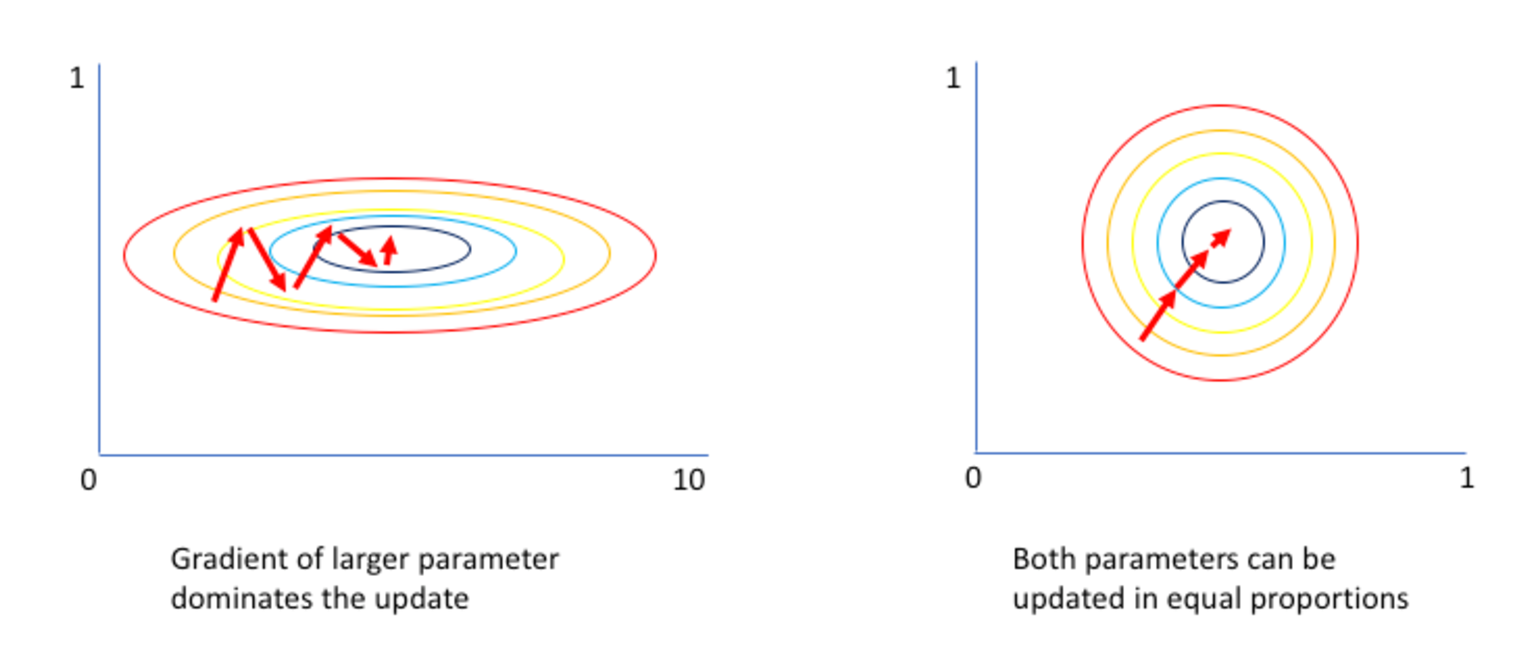
\includegraphics[width=0.5\textwidth]{Cap5/inputnorm.eps}
	\caption{Intuition behind input normalization}
	\label{inputnormfig}
\end{figure}

\subsubsection{Neural Network}
As an actor-critic model, we have two networks: one for the value function and other for the policy itself. They have the same architecture: two layer, fully connected, with 64 neurons in each hidden layer and hyperbolic tangent as activation function. The architecture is illustrated in Figure \ref{rlnetwork}. Table \ref{tab:rl_network_summary} summarizes the parameters in this new architecture, also considering the parameters from the Gaussian Action Space Noise, described in \ref{gasp}.

\begin{figure}[!htbp]
	\centering
	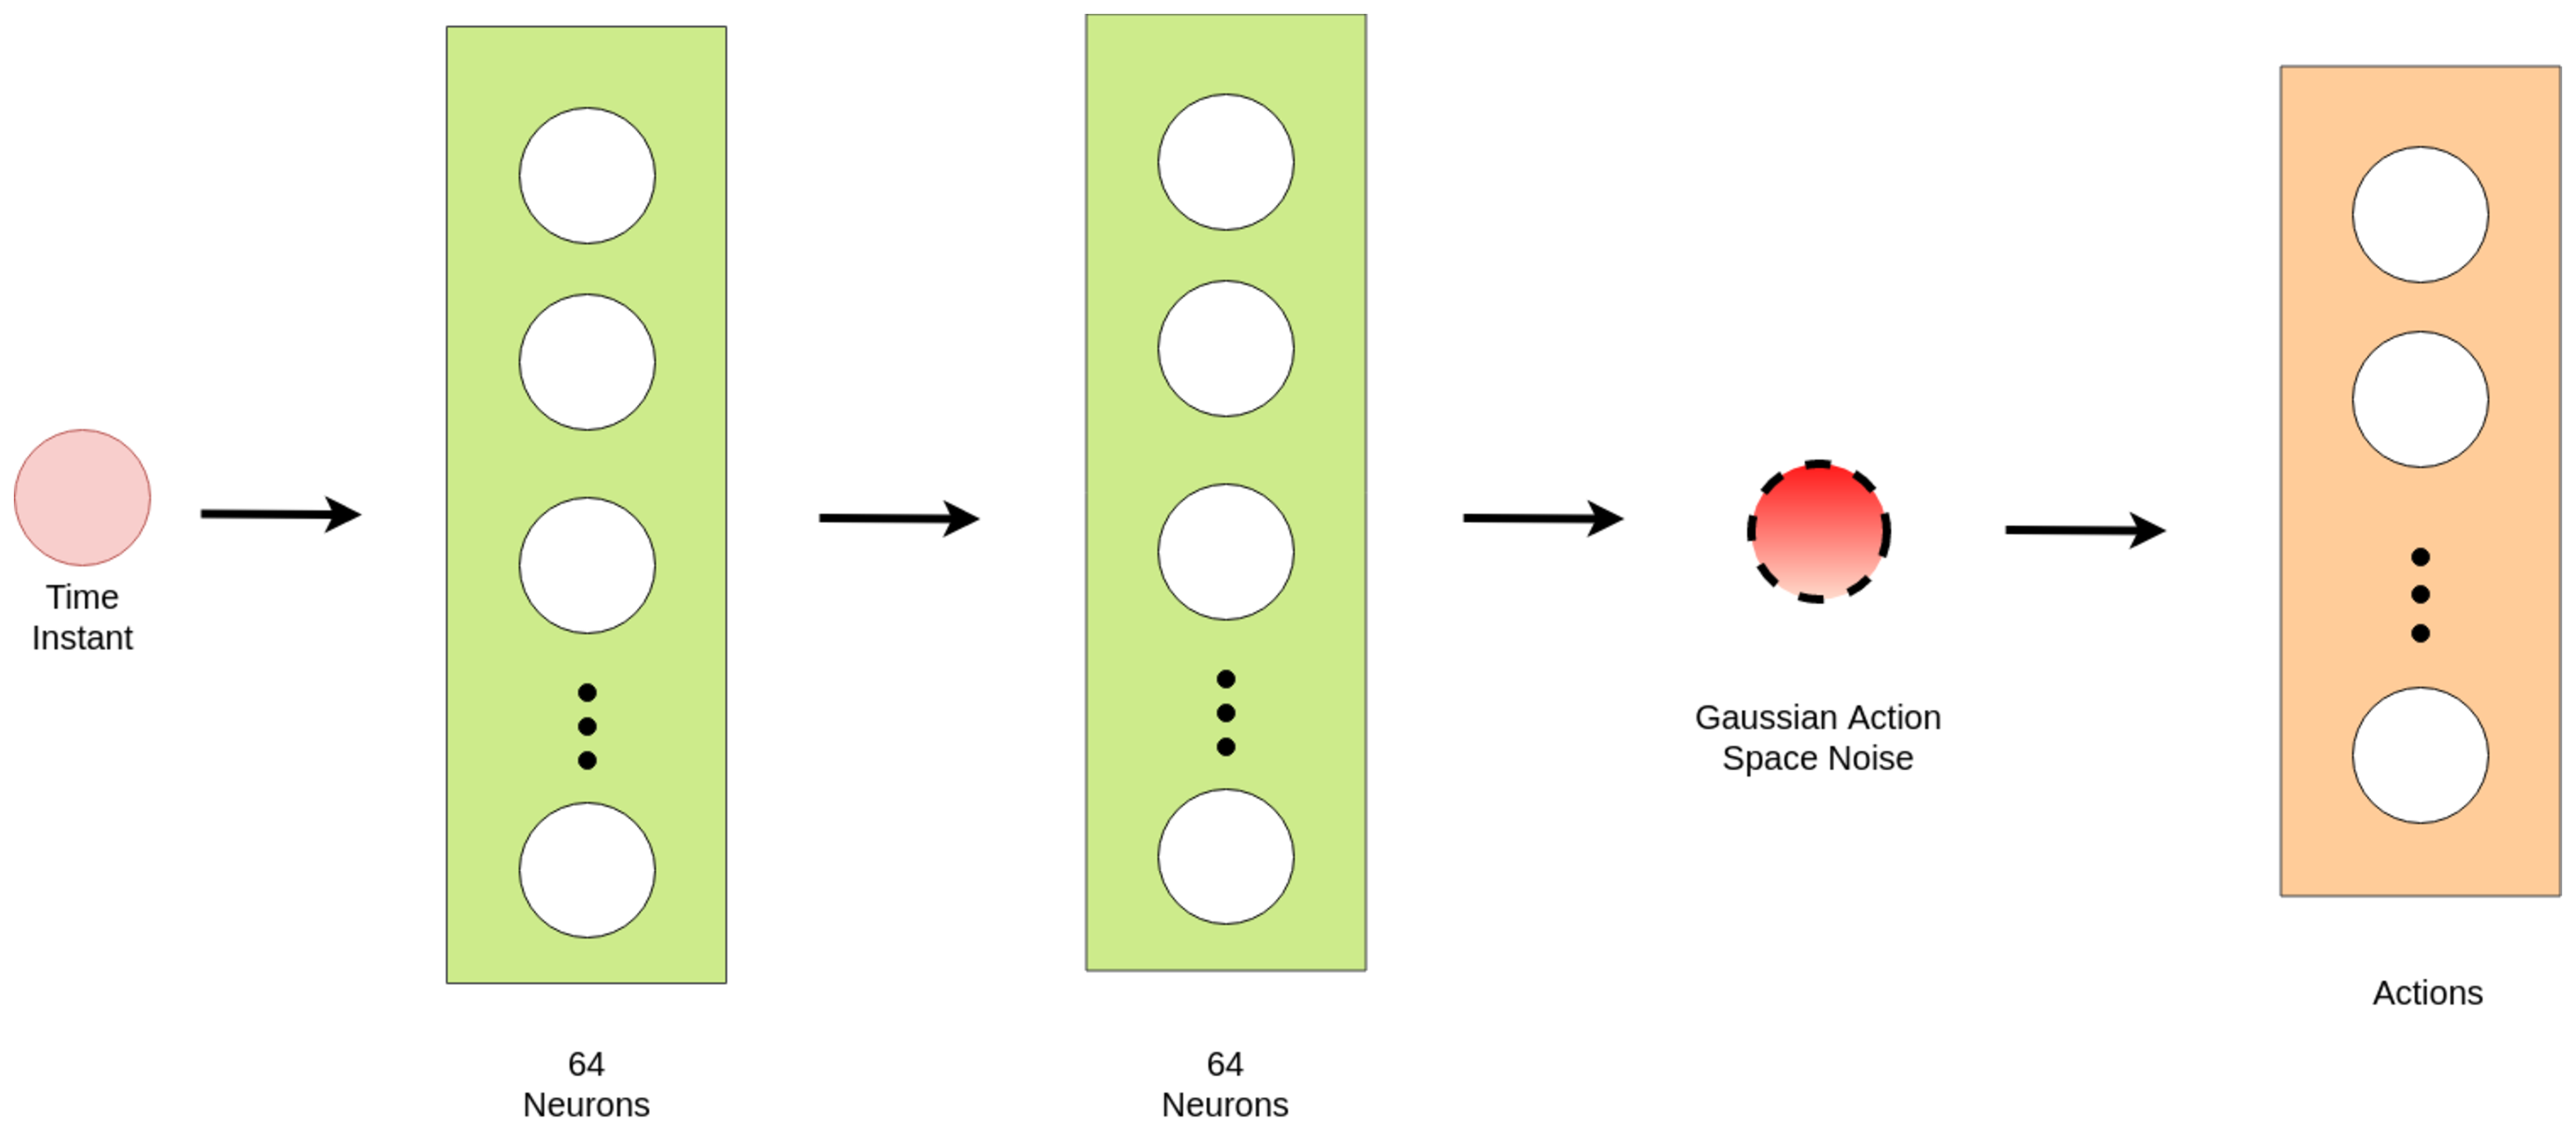
\includegraphics[width=0.5\textwidth]{Cap5/rlnetwork.eps}
	\caption{Architecture used by pure Reinforcement Learning models.}
	\label{rlnetwork}
\end{figure}

\begin{table}[htbp]
	\caption{The Reinforcement Learning Network Summary}
	\begin{center}
		\begin{tabular}{|c|c|c|c|}
			\hline
			\textbf{Layer}&{\textbf{Neurons}}& \textbf{Activation}& \textbf{Parameters} \\
			\hline
			Dense & 64 & $tanh$ & 128  \\
			\hline
			Dense & 64 & $tanh$ & 4160 \\
			\hline
			Output & 23 & Linear & 1495 \\
			\hline
			Noise & 23 & Linear & 23 \\
			\hline
		\end{tabular}
		\begin{tabular}{|c|c|}
			\hline
			\textbf{Total Parameters} & 5806 \\
			\hline
		\end{tabular}
		\label{tab:rl_network_summary}
	\end{center}
\end{table}


\subsubsection{Gaussian Action Space Noise}\label{gasp}

The last idea explored in this policy representation is the Gaussian action space noise for better exploration. It adds adaptive noise to the action space of the neural network. Discrete RL uses $\epsilon$-greedy \cite{Watkins:1989} to confer exploration. Gaussian action space noise injects normal randomness directly into the actions of the agent, altering the types of decisions it makes and helping algorithms explore continuous environments more effectively. The Figure \ref{gaussiannoise} illustrates this technique.


\begin{figure}[!htbp]
	\centering
	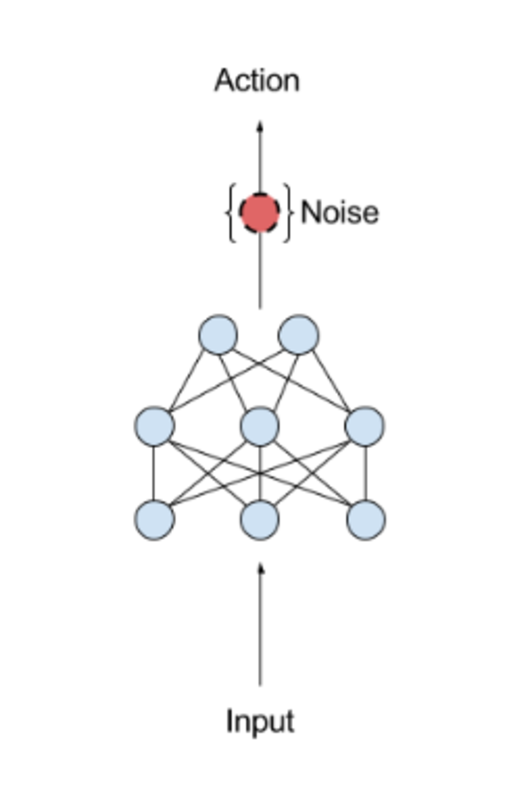
\includegraphics[width=0.3\textwidth]{Cap5/gaussiannoise.eps}
	\caption{Gaussian noise applied to action space to ensure better exploration in continuous environments.
	\cite{parameternoiseblog}
	}
	\label{gaussiannoise}
\end{figure}

\subsection{Task Description}
The learning task consists in the activity the agent will execute in order to achieve the expected behavior through the policy. In this experimentation, we would like to learn the kick motion. Therefore, is straightforward that the scenario is based on kick the ball.

The agent is started in a fixed position of the soccer field. The ball, on the other hand, starts in a position $\alpha_{ball}$ meters from the agent, in front of him. The parameter $\alpha_{ball}$ can be optimized in order to decide the best position the agent have to stop to kick the ball better. However, for this experimentation, we fixed its value.

We repeat the following flow: in the beginning of the episode, all the joints are initialized in a certain value that correspond to the joints the robot assume when it stops to walk and will start the kick motion. Then, we start the learning steps, applying the joints from the neural network to the robot. When we use RISD, there's a intermediate phase executing the reference motion, as described in \ref{risd}.

After the execution of those steps, we finalize the episode turning all the joints to zero. When there's no Early Termination, this happens after a fixed number of steps that we can ensure the motion has over. Otherwise, this occurs when the early termination condition is reached.

Figure \ref{taskdescription} shows the tasking running.


\begin{figure}[!htbp]
	\centering
	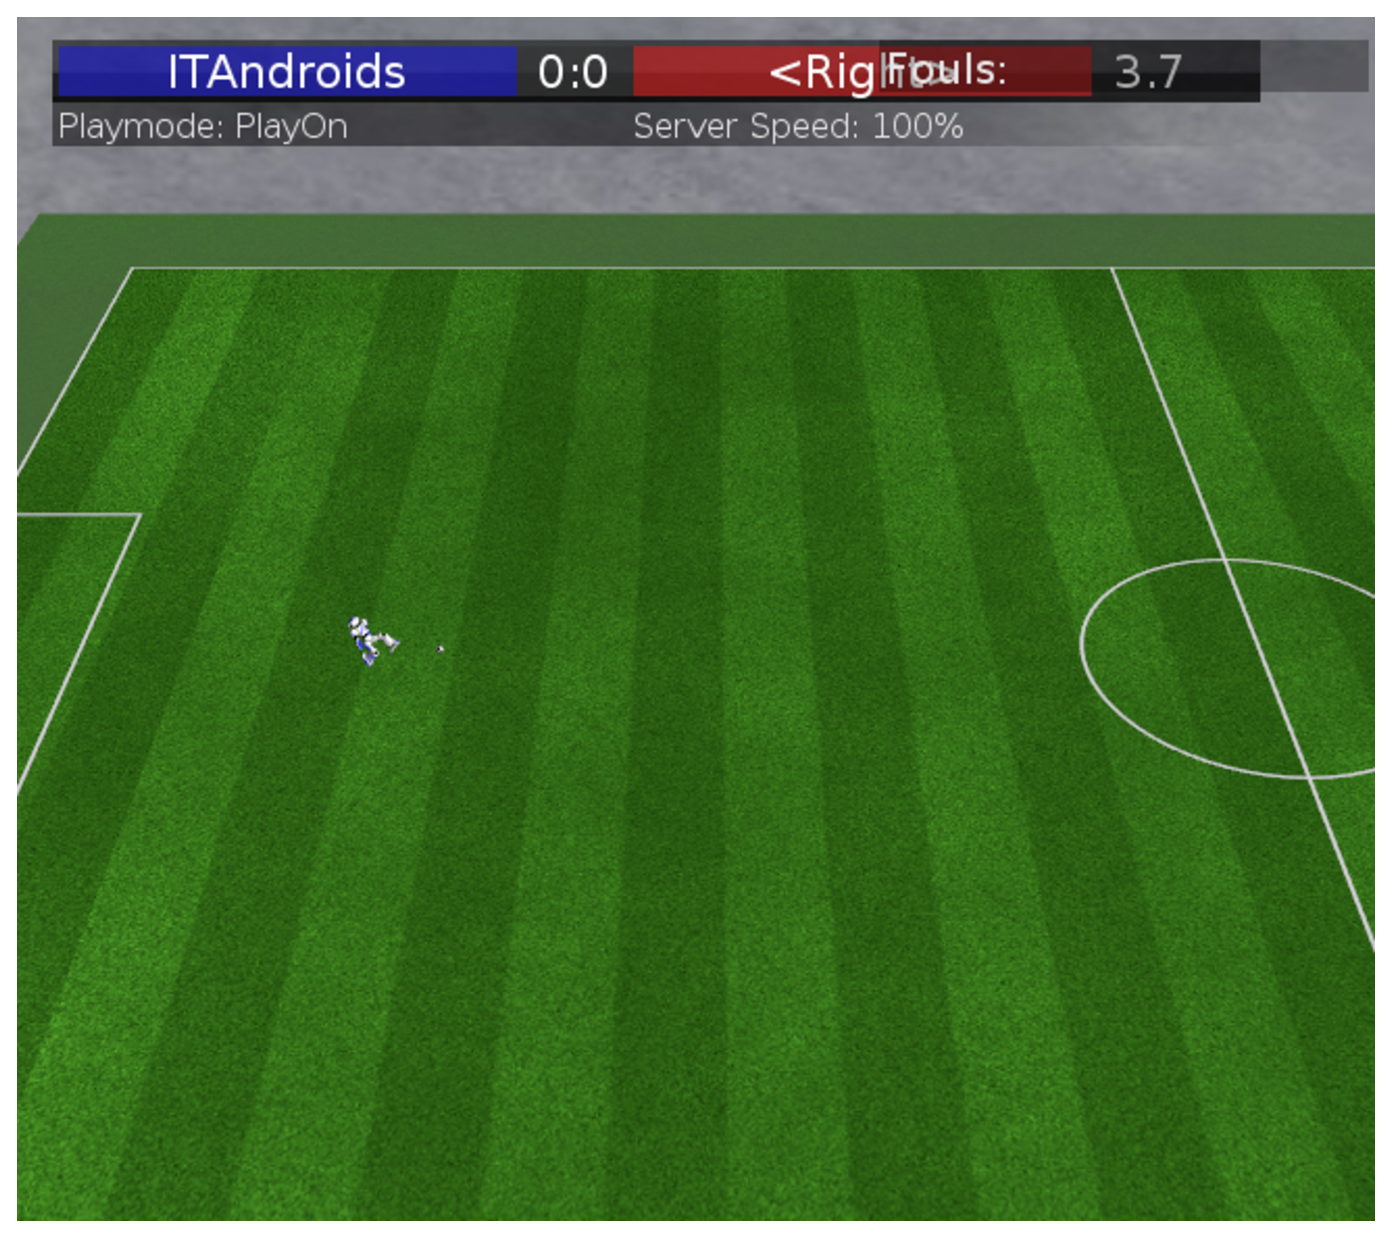
\includegraphics[width=0.7\textwidth]{Cap5/taskdescription.eps}
	\caption{Task used to learning kick motion.}
	\label{taskdescription}
\end{figure}

\section{Infrastructure}
\subsection{Reinforcement Learning Server}\label{rlarchitecture}

Figure \ref{rlserver} shows the architecture used to integrate the learning algorithm, agent and simulation environment. The simulation server exposes a state to the soccer agent, which model this information and passes to the learning algorithm that chooses a action accordingly and returns to the agent. Then, it applies this action in the environment, modifying its state, completing the cycle.

\begin{figure}[!htbp]
	\centering
	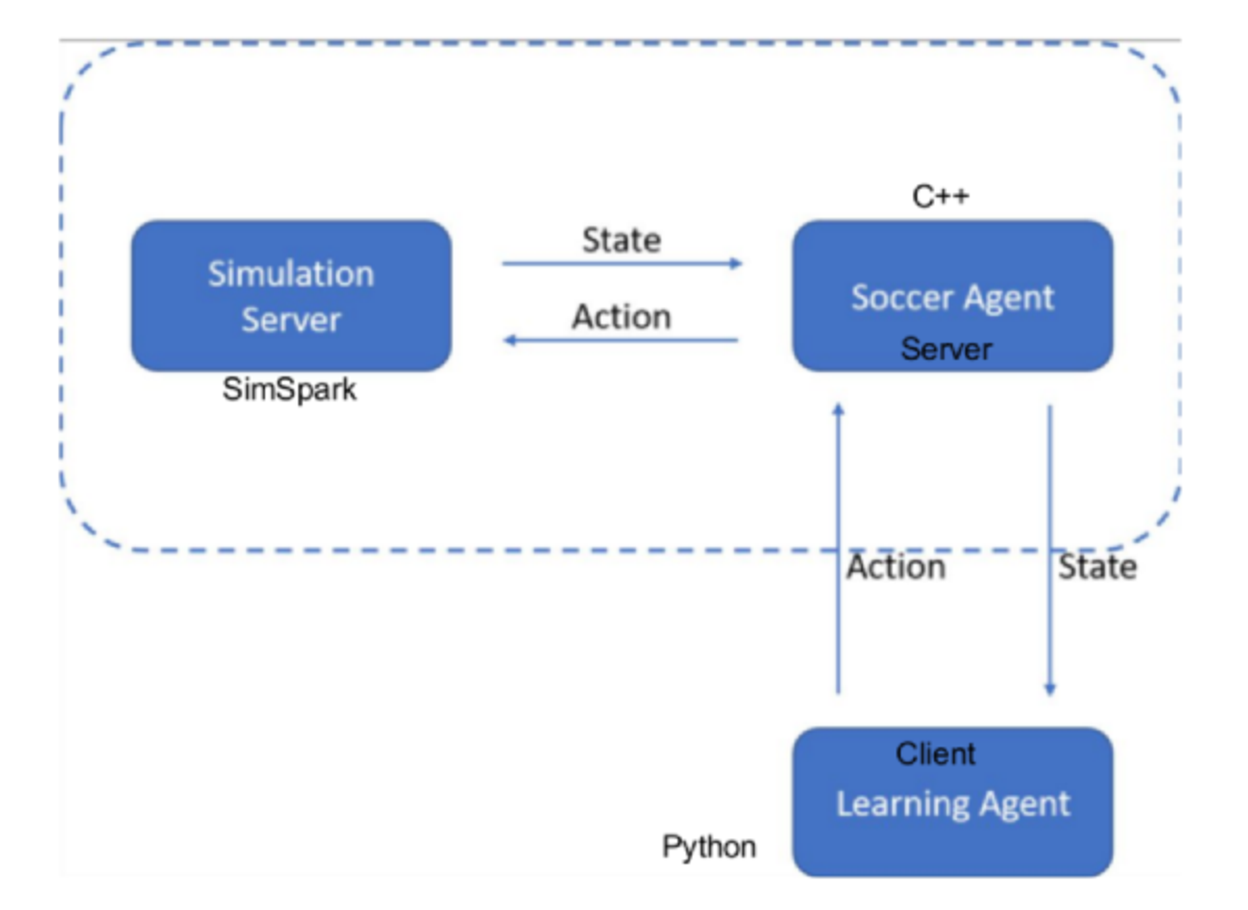
\includegraphics[width=0.3\textwidth]{Cap5/rlserver.eps}
	\caption{Reinforcement Learning Server Architecture.
		\cite{tgmuzio}
	}
	\label{rlserver}
\end{figure}

\subsubsection{Simulation Server}

The simulation environment used, as mentioned before, is Simpark. It uses a TCP Socket to communicate with the agent and exposes a interface for querying the ground truth state for many features from the agent - which can be helpful to state evaluation and avoids to use agent's perceived data that has noise. 

\subsubsection{Soccer Agent}
The agent used is from ITAndroids Soccer 3D team and it leads with the perception information sent from the server, model the world with this information and make decisions accordingly. Additionally, there's a entity, called Wizard, whose purpose is query the ground truth state. All this code is written in C++ and the task described in \ref{taskdescription} was implemented in the agent itself.

Other tool that worth mention is RoboViz, a publicly available visualization tool that allows a few improvements over the default visualization tool. We used it to verify if the task was implemented successfully.

\subsubsection{Learning Agent}\label{learningagent}

We created another interface to integrate the Soccer Agent with the algorithms used in this experimentation. These were implemented by OpenAI Baselines \cite{baselines}, a repository of high-quality implementations of reinforcement learning algorithms whose purpose is make easier for the research community to replicate, refine, and identify new ideas, and create good baselines to build research on top of. The community developed those algorithms using Python language with the Tensorflow \cite{tensorflow2015-whitepaper} framework.

This integration was done using gRPC \cite{grpc}, an open source remote procedure call (RPC) system that generates cross-platform client and server bindings. It uses HTTP/2 for transport and Protocol Buffers \cite{protocolbuffers} as the interface description language, serializing structured data.




\subsection{Neural Network Deployment}

When we use the architecture from \ref{rlarchitecture}, two problems related to the neural network deployment arise.

The first one is related to the HLM. We have a supervised learning model trained using the framework Keras outside the environment and with no relation to OpenAI Baselines. Therefore, we need a way to import this model from Keras model into the learning algorithms.

The second problem is to deploy the network from learning algorithm to the soccer agent. When the network is trained using OpenAI Baselines, there's no contact between the soccer agent and the model. As described in \ref{learningagent}, there's a interface to communicate the actions between them. All calculations happens in only one side. However, during a game, it's not possible to maintain this dependency, so we need a way to run the network inside soccer agent and without the whole training structure.

\subsubsection{Import Supervised Model into OpenAI Baselines}

To solve this problem, it's important to understand how Keras works and what's the challenge behind this import. 

Keras works on top of lower level machine learning frameworks. Its purpose is make easier to prototype and train models with few lines of code. With Keras, developers don't need to understand in deep how computational graphs works and some math behind the models. Actually, this framework wraps code from the lower level ones. Therefore, even being easier to use, all the computation and data structures remains the same.

As back-end framework that Keras runs on top of, we used Tensorflow. As described previously, it creates a computational graph with math tensors as inputs that "flow" inside and returns the expected result.

Given that context, the idea is straightforward: we create a "Kick Policy" class, that creates the model using Keras, load its weights, gets the output tensor and injects in the rest of Tensorflow's computational graph related to the learning algorithm. The Algorithm \ref{importnetworkpseudocode} explains sequentially this idea.

\begin{algorithm}
	\caption{Import Keras model into Tensorflow}
	\begin{algorithmic} 
		\REQUIRE Keras output model
		\STATE $model \leftarrow createKerasModelStructure()$
		\STATE $model.load\_weights(keras\_output\_model)$
		\STATE $outputTensor \leftarrow model.output$
		\STATE Inject $outputTensor$ in the rest of computational graph
	\end{algorithmic}
	\label{importnetworkpseudocode}
\end{algorithm}

It's important to mention that the $load\_weights$ operation already initializes the graph variables and if we initialize them again, we lose the pre-trained weights.

The biggest problem of this integration is we can't use Input Normalization Filter and Gaussian Action Space Noise, described in \ref{sec:inputnorm} and \ref{gasp}, respectively. Therefore, we can face gradient and exploration problems during learning.

\subsubsection{Export OpenAI Baselines onto Soccer Agent}

As mentioned earlier, Tensorflow creates a data flow graph with all operations executed during the algorithm. Figure \ref{fig:dataflowgraph} shows the whole graph for PPO used in this experimentation. However, we need to export only the policy network itself.

\begin{figure}[!htbp]
	\centering
	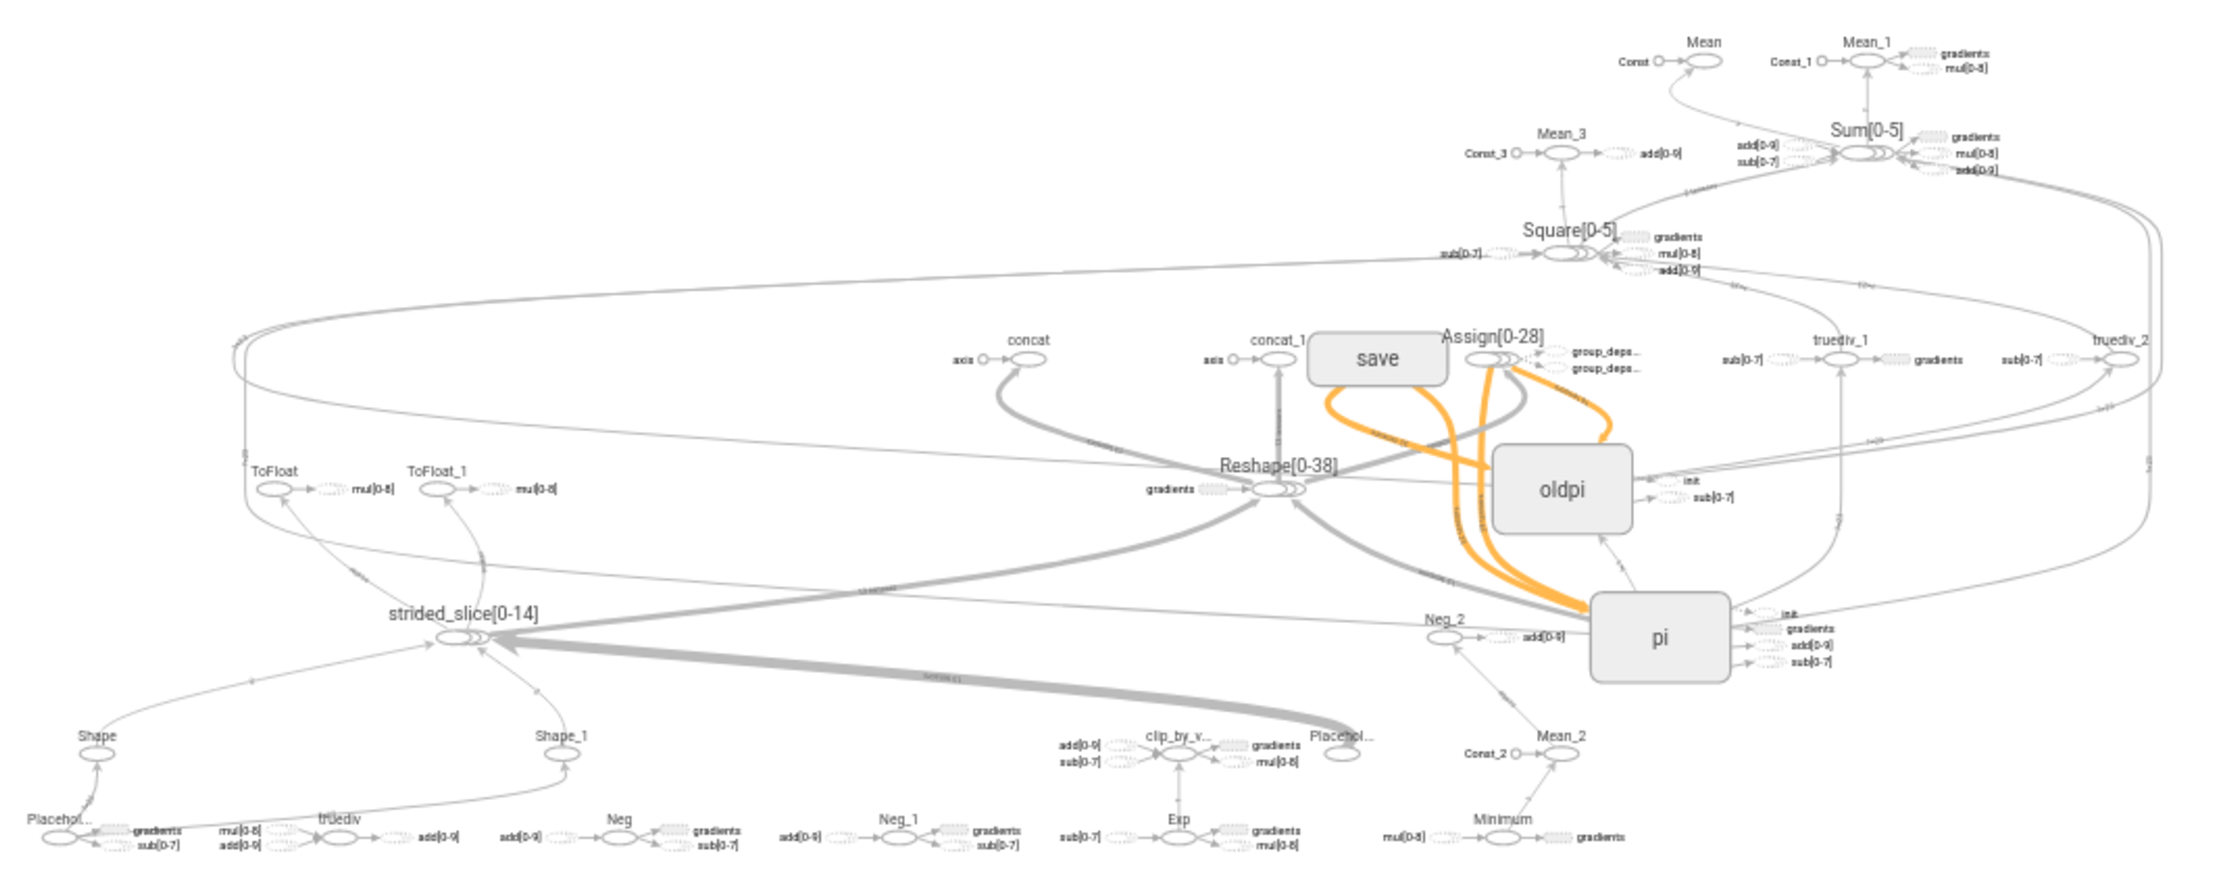
\includegraphics[width=1.1\textwidth]{Cap5/dataflowgraph.eps}
	\caption{Data flow graph for PPO algorithm.
	}
	\label{fig:dataflowgraph}
\end{figure}

It is important to mention that ``policy network" mean only the neural network that maps state to actions, and not the whole policy node ``pi" in Figure \ref{fig:dataflowgraph}. The ``pi" node also have the value function network and gaussian noise in action space, only needed during the learning process. Figure \ref{fig:pigraph} shows the whole ``pi" node.

\begin{figure}[!htbp]
	\centering
	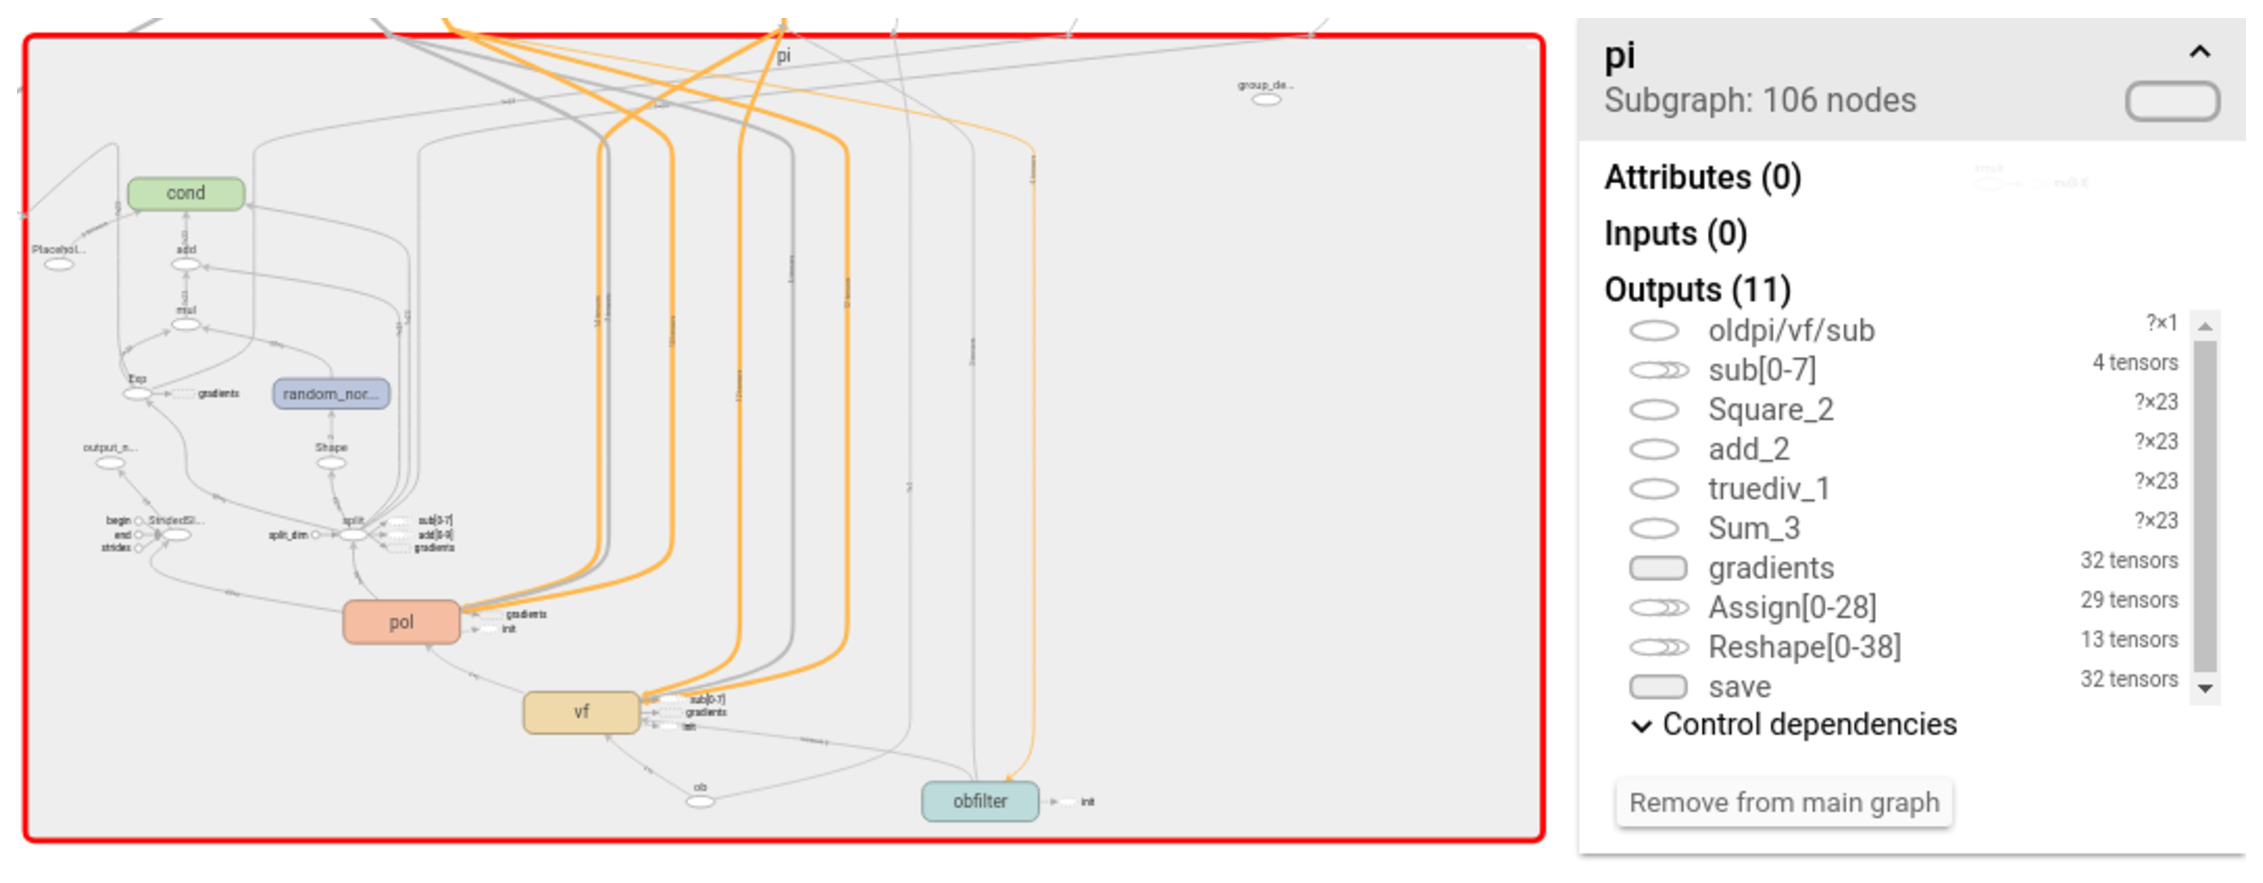
\includegraphics[width=1.1\textwidth]{Cap5/pigraph.eps}
	\caption{ ``Pi" data flow node from PPO.
	}
	\label{fig:pigraph}
\end{figure}

Therefore, to export this policy network, we need to add a new "identity" node in the output from that. This node has the same resultant tensor, but it is possible to label it and we can freeze the subgraph whose output is the labeled node itself. Internally, Tensorflow will start freezing the output node and its dependencies, recursing until input nodes. Then, we save this data structure in a proto file that we read using the C++ API in the soccer agent. Figure \ref{fig:policygraph1} and \ref{fig:policygraph2} show the policy data flow graphs from Figures \ref{rlnetwork} and \ref{fig:model_plot}, respectively.



\begin{figure}[!htbp]
	\centering
	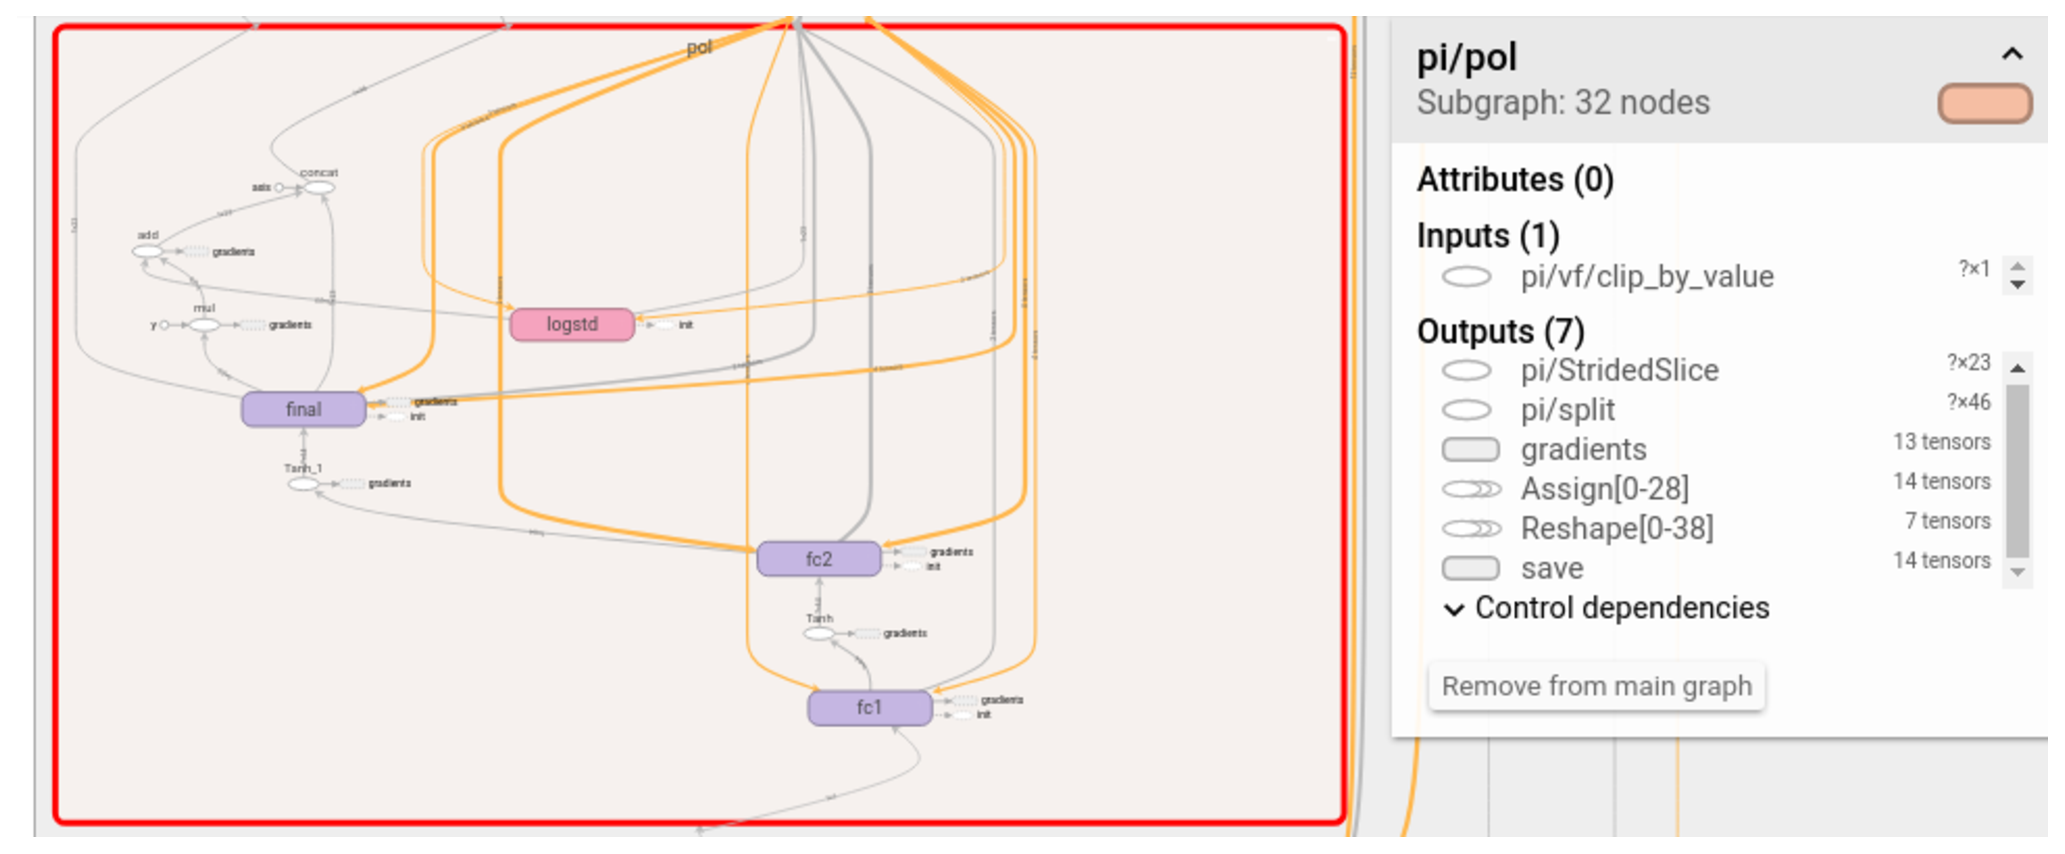
\includegraphics[width=1.1\textwidth]{Cap5/policygraph1.eps}
	\caption{ Policy data flow graph from Figure \ref{rlnetwork}
	}
	\label{fig:policygraph1}
\end{figure}

\begin{figure}[!htbp]
	\centering
	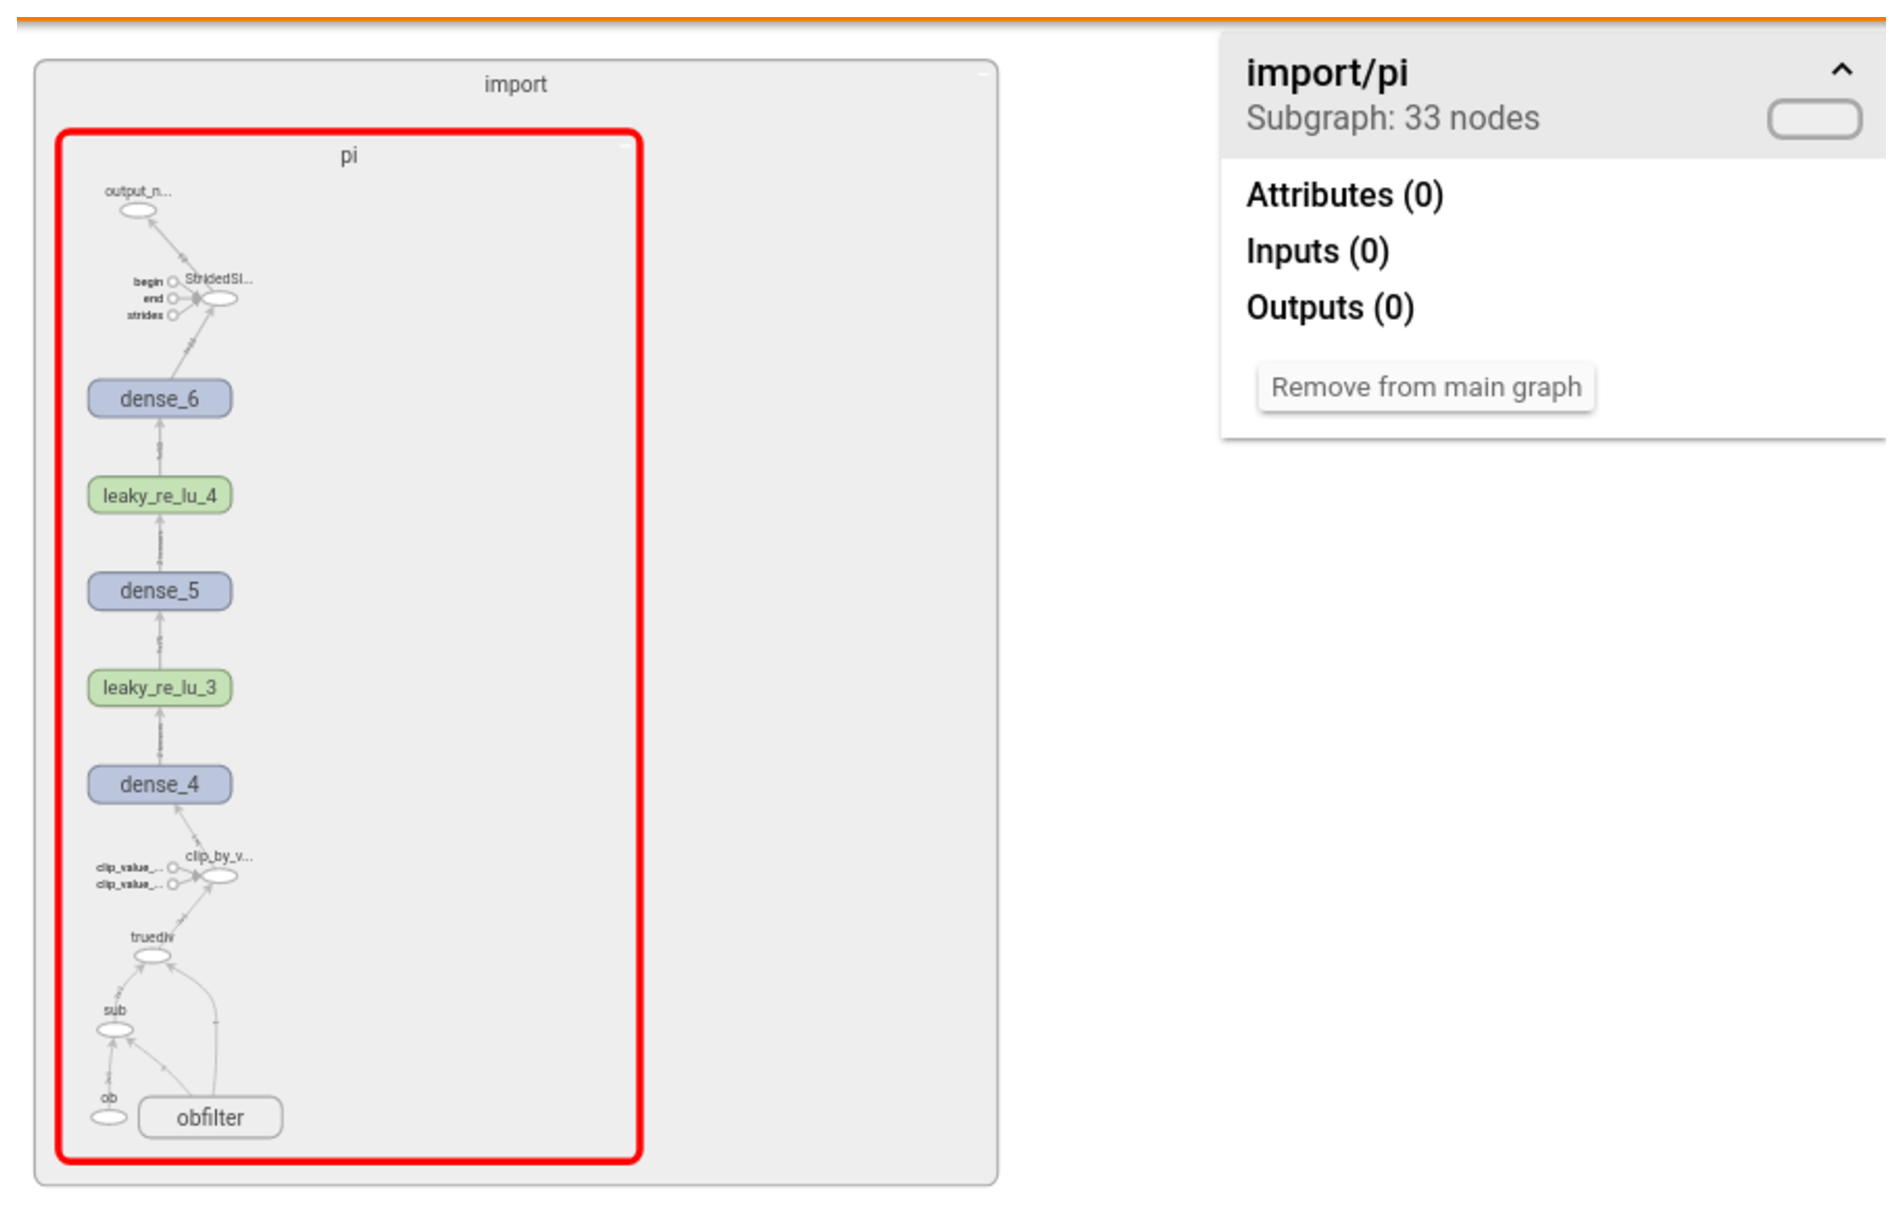
\includegraphics[width=1.1\textwidth]{Cap5/policygraph2.eps}
	\caption{ Policy data flow graph from Figure \ref{fig:model_plot}
	}
	\label{fig:policygraph2}
\end{figure}


\subsection{Distributed Training}
Reinforcement Learning training is much more costly computationally when compared to the supervised one described in \ref{supervised_learning_setup}. Additionally to the costs of applying gradients in the network, we need to gather all the data from agent simulations. Furthermore, since the data distribution changes during the learning, it's harder to converge, se it is needed a large amount of data.

In this context, use a single agent to get all the data and train the algorithm takes too long time to converge and, depending of the problem, it is not viable. We need a way to get more data faster and accelerate the training.

\subsubsection{Data Parallelism}

The solution for this challenge is distribute the training using several agents. Each agent interacts with its own environment, but the results are applied to the same network. This technique is called Data Parallelism, because the parallelization happens in data gathering. It opposes the idea of Model Parallelism, where the learning model itself is distributed, but this technique is not interesting in reinforcement learning training.

In Data Parallelism, we applied a master-workers architecture, as shown in Figure \ref{fig:master-worker}. It has several worker nodes, whose job is gather data by simulating the agent, and a master node, which controls the learning algorithm. This architecture works very well in this experiment because the computation from workers are very similar so we can conduct several independent processes in those. It can also be fault tolerant: if one worker dies, the learning process can keep running.

\begin{figure}[!htbp]
	\centering
	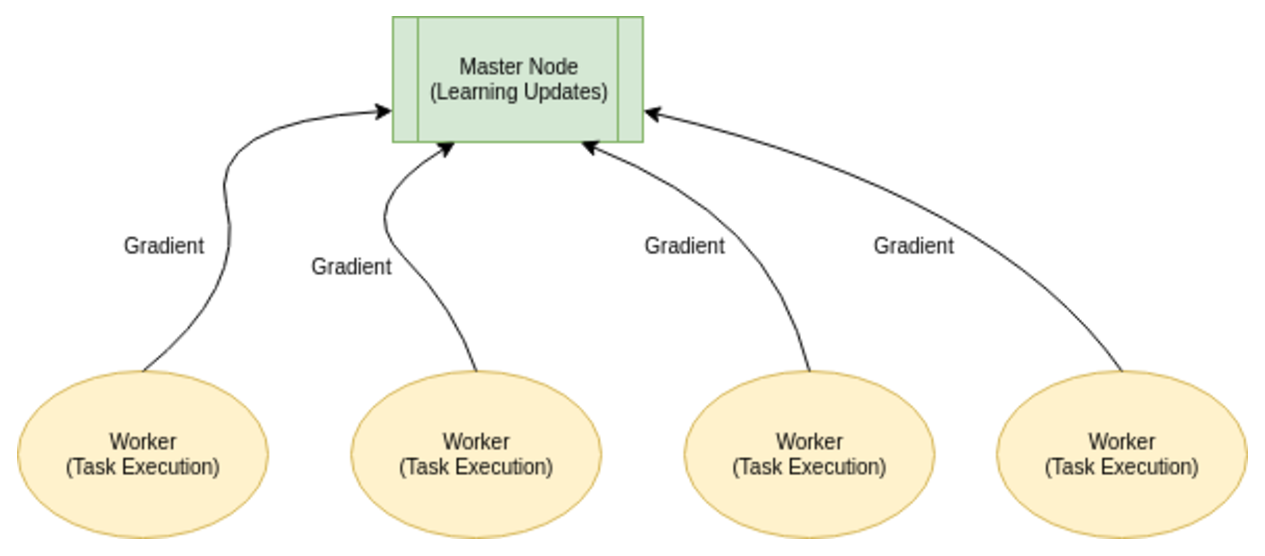
\includegraphics[width=1.1\textwidth]{Cap5/master-worker.eps}
	\caption{ Master-workers architecture for data parallelism.
	}
	\label{fig:master-worker}
\end{figure}

\subsubsection{Synchronous vs. Asynchronous Distributed Training}

There are two ways to apply updates from a master-workers architecture in the learning algorithm. Both ways are illustrated in Figure \ref{fig:distributedtraining}.

In asynchronous training, each worker executes the task, gathers data, calculate the gradient and apply it in the neural network. There's no interaction between workers so the learning updates can occur freely and, therefore, faster. However, the downside is that each worker has its own version of the network which can cause a discrepancy between them and slows the convergence.

On the other side, in the synchronous training, each worker executes the same job as the asynchronous one. However, the master node collects the gradients and applies an average from them. In this way, the updates occurs in the same frequency, but they are much more precise (and therefore we can use large learning rates). 

\cite{heess2017} implemented a variation of PPO called Distributed PPO (DPPO) and their experiments shows that synchronous updates worked better in practice. Hence, in this experimentation we also used this type of distributed training.

\begin{figure}[!htbp]
	\centering
	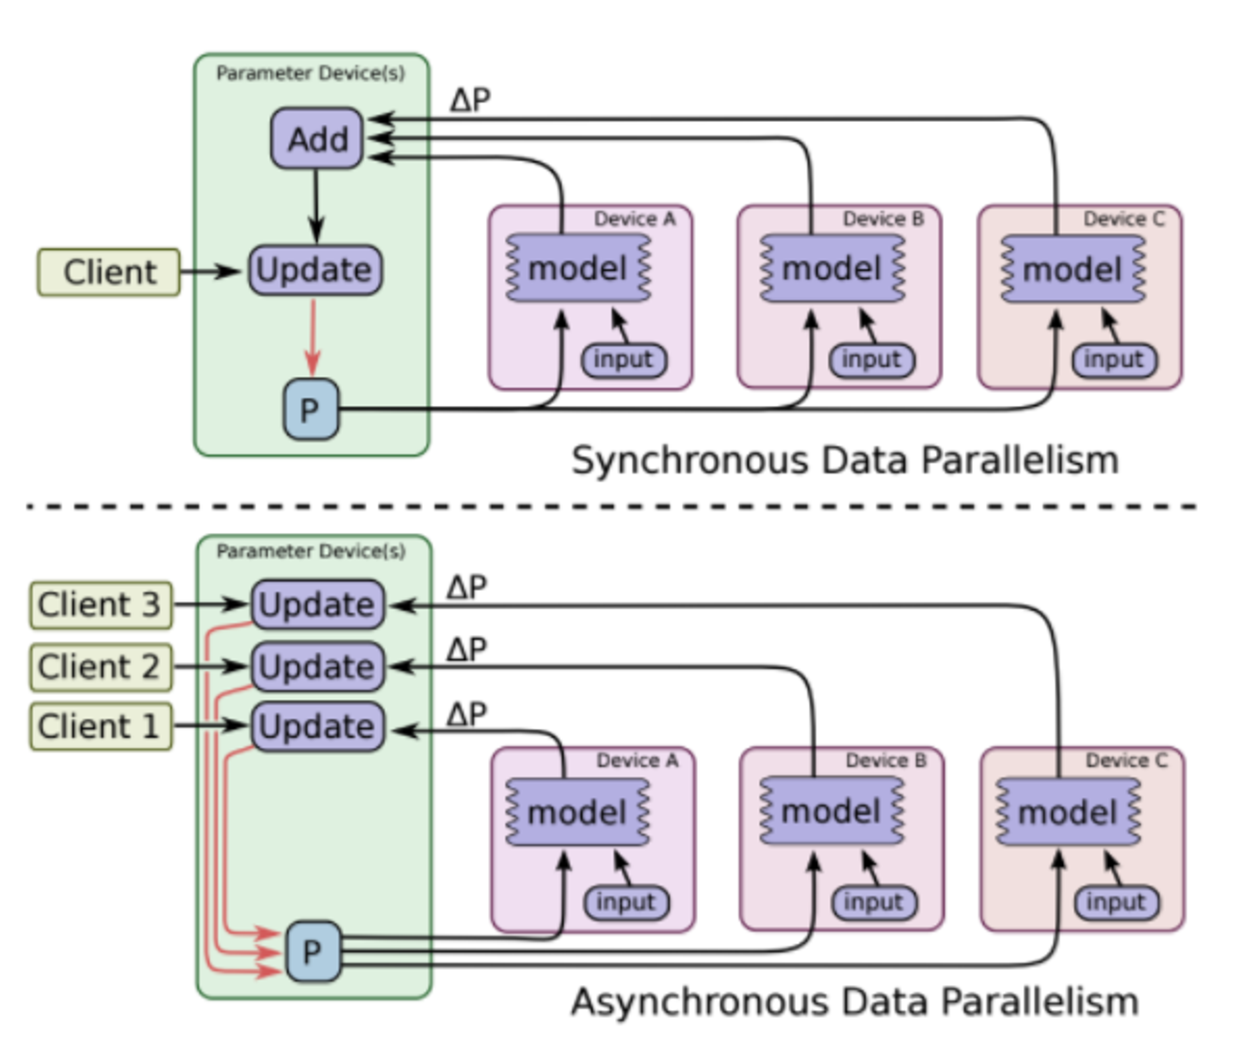
\includegraphics[width=0.8\textwidth]{Cap5/distributedtraining.eps}
	\caption{ Synchronous and Asynchornous Distributed Training.
	}
	\label{fig:distributedtraining}
\end{figure}

\subsection{Metrics}

We need evaluation metrics to compare the techniques in section \ref{sec:experimentation_setup}. Several of them were collected and described below:

\begin{itemize}
	\item \textbf{Episode Reward Mean}: This metric is the mean of cumulate reward during the whole episode. It's directly related to the motion performance. Then, it's the main metric in the comparison.
	\item \textbf{Value Function Loss}: Says how good is the prediction of value function by the network.
	\item \textbf{Timesteps So Far}: It means how many cycles (observation-action-reward) have been executed. This metric was used to compare the speedup from distributed training.
	\item \textbf{Episode Length Mean}: In the case of models with no fixed length, this metric will allow us to understand how the learning worked.
\end{itemize} 

\subsection{Monitoring via Tensorboard}
Lastly, we need a tool whose purpose is monitor the metrics collected during the training. We used Tensorboard \cite{tensorboard}, a graphic visualizer tool from Tensorflow. Figure \ref{fig:tensorboard} shows the GUI with some metrics. Using that, we can compare several models and their metrics, visualize computational graphs and debug the learning process.

\begin{figure}[!htbp]
	\centering
	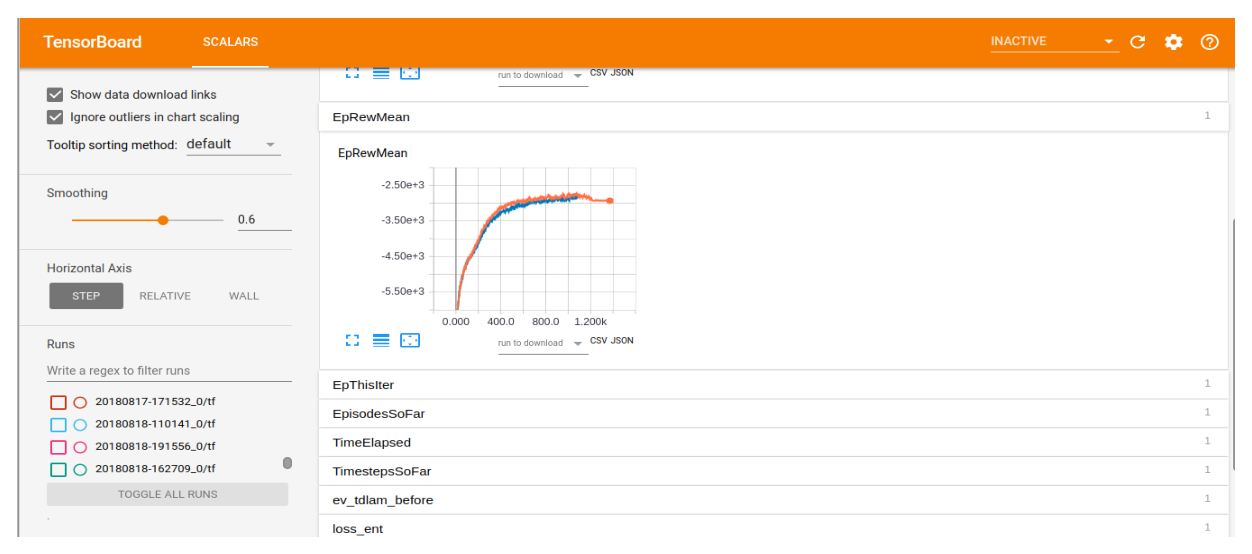
\includegraphics[width=1.0\textwidth]{Cap5/tensorboard.eps}
	\caption{ Monitoring training metrics with Tensorboard.
	}
	\label{fig:tensorboard}
\end{figure}

\chapter{Results' Analysis and Discussion}\label{ch:results}
\section{Distributed Training}

The first results we show here is regarding of data parallelism by the adoption of distributed training. As described in section \ref{sec:distributedtraining}, in RL training we used a master-worker model with \textbf{108 agents} collecting data in parallel.

We used Intel AI DevCloud \cite{inteldevcloud}. It is a cluster of Intel Xeon Scalable Processors that assists with machine learning and deep learning research, with several optimizations for this domain. We had available 9 computation nodes, each of them with 24 cores for processing. Therefore, we trained using 8 nodes for workers (each of them with 4 agents) and one node for master computation. All the scripts used for training configuration are available in github repository\footnote{\label{scripts} https://github.com/luckeciano/deep-rl-humanoid-kick} of this work. 

In Figure \ref{fig:parallelism}, we see how the data collection had improved by using distributed training in AI DevCloud. In this graph, we have the number of samples collected by learning update in a training using the distributed configuration and other in a local training with a single agent. If we consider the same instant at each experimentation (i.e, after the same period of time), we can quantify the speedup:

\begin{equation}
	SpeedUp \approx \frac{4.58 * 10^{8}}{4.59 * 10^{6}} \approx \textbf{100}
\end{equation}

In this comparison, we have a speedup of 100. It worth mentioning that this number can vary depending on the training itself, because the computation will change over time. For example, if during training the episode length tends to grow, the time simulating agents have the same behavior.


In Figure \ref{fig:absdatacollection}, we consider the best scenario for data collection from those experimented. In the graph, there is the number of samples collect by the time.
In this example, we have collected approximately \textbf{740 millions of samples} in eight hours. It means \textbf{92.5 millions of samples by hour}. Each of them means a cycle of 20 milliseconds in the simulation server. Therefore, we collected approximately \textbf{21.4 days of real time training in each hour of simulation}. The training from Figure \ref{fig:absdatacollection} collected approximately \textbf{171 days of uninterrupted training} -- almost half year.

\begin{figure}[!htbp]
	\centering
	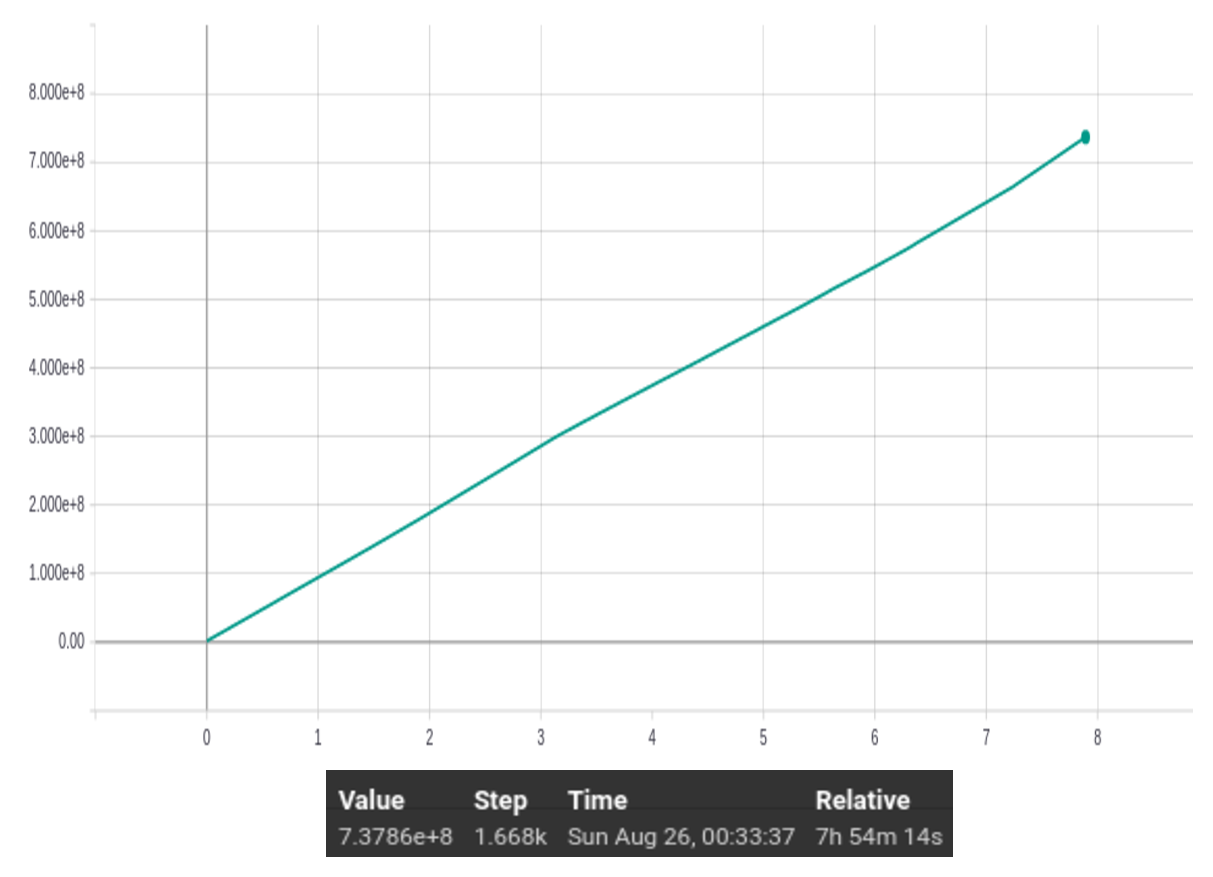
\includegraphics[width=1\textwidth]{Cap6/absolutedatacollection}
	\caption{Data collection in best scenario}
	\label{fig:absdatacollection}
\end{figure}



\section{Pure Reinforcement Learning methods results}

In this section, we show the results regarding of RL experiments. We tested several scenarios using the experimentation setup described in Section \ref{sec:experimentation_setup}. All the hyperparameters from each experiment can be found in the Appendix \ref{app:hyperparameters}.

\subsection{RNR}

The first model we experimented is RNR. In this, we started from randomly distributed weights in a neural network and, by using RL, we achieved a motion that not follows a well-defined human kick behavior, but is able to inject some velocity to the ball. Figure \ref{fig:rnrreward} shows how the reward improves over learning update.

\begin{figure}[!htbp]
	\centering
	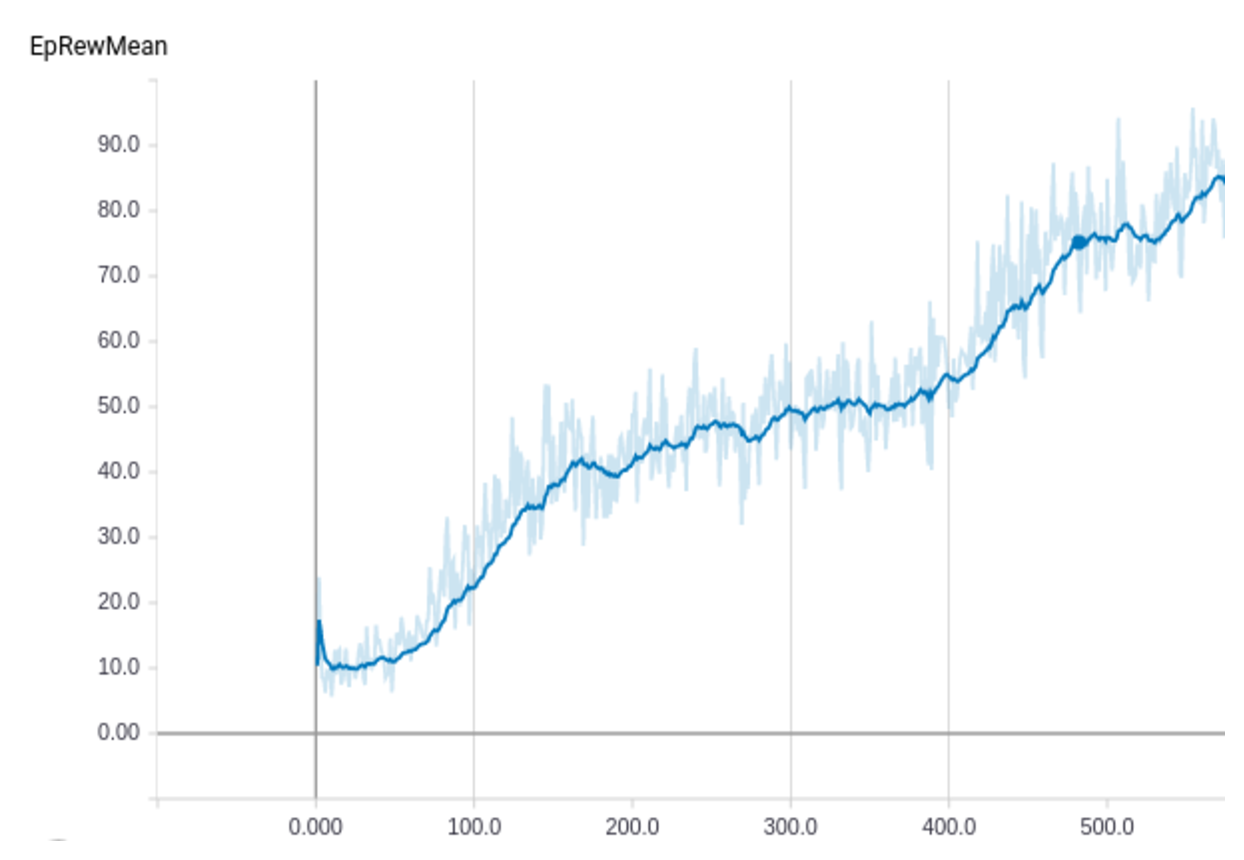
\includegraphics[width=0.8\textwidth]{Cap6/rnrreward.eps}
	\caption{RNR Reward Curve by learning update}
	\label{fig:rnrreward}
\end{figure}

Other experimentation sessions shown us that RNR tends to converge to the maximum value presented in Figure \ref{fig:rnrreward}.

We also encountered a problem during the optimization process: Simspark simulation tends to drastically drop the reward to zero after approximately 4 or 5 hours of training in certain experiments. We didn't found a reason but when we restart training from the previous session, the problem just disappear. We opted to not show this issue in results to not compromise the focus of the research.

Figure \ref{fig:rnr_kick_sequence} shows RNR resultant motion. It is possible to see that the behavior is different from human kick pattern. Basically, the robot jumps and push its right leg in ball direction. This kick runs between two to four meters straight. The animation can be seen in the repository.

\begin{figure}[!htbp]
	\centering
	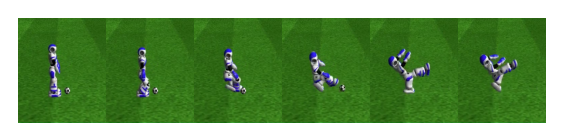
\includegraphics[width=0.8\textwidth]{Cap6/rnr_kick_sequence.eps}
	\caption{RNR kick motion sequence.}
	\label{fig:rnr_kick_sequence}
\end{figure}

\subsection{RRR}

It the context of optimization is difficult to the agent explore the whole action space and mimics a human behavior of kicking. To address this challenge, we used the reference motion also used in supervised learning section.

When we train just using this reward -- without any reward to kick the ball itself -- the robot achieves a interesting behavior: it remains stopped, even growing the reward, as in Figure \ref{fig:rrrreward}.

\begin{figure}[!htbp]
	\centering
	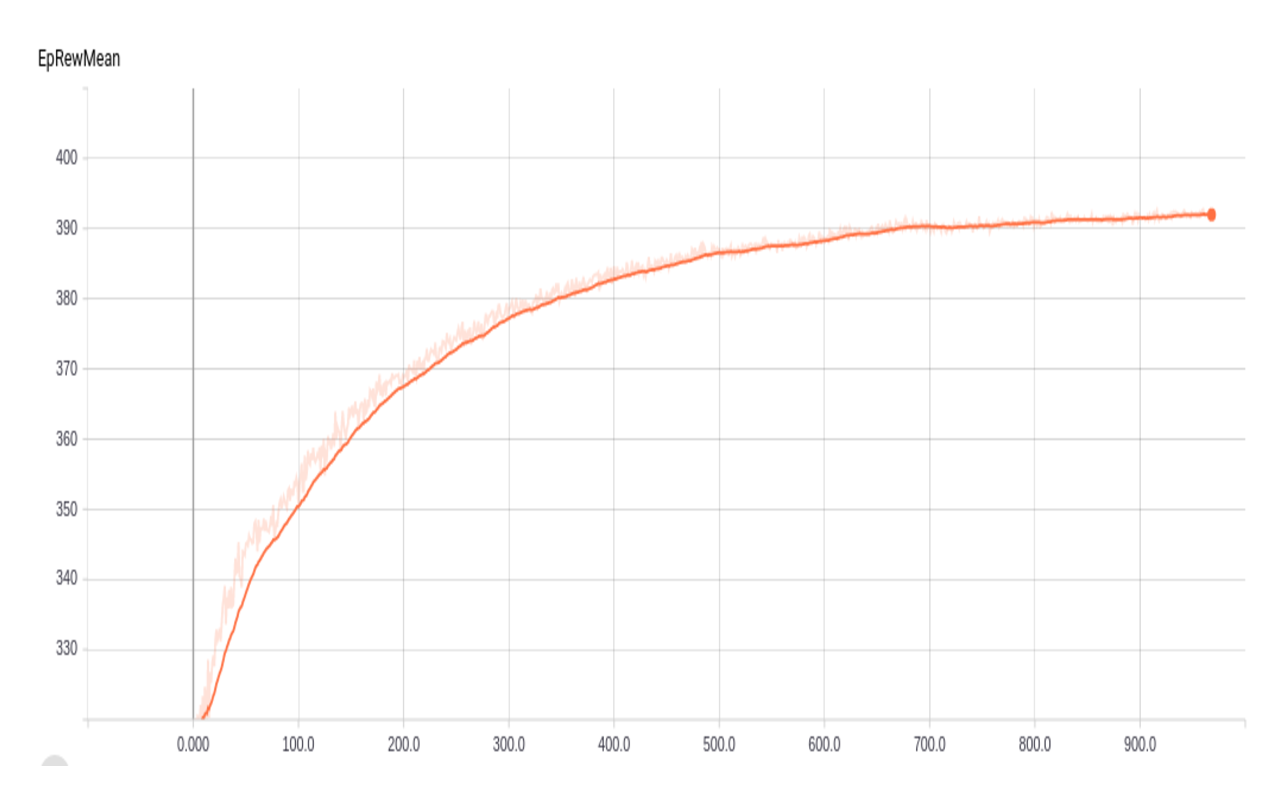
\includegraphics[width=0.8\textwidth]{Cap6/rrrreward.eps}
	\caption{RRR Reward Curve by learning update}
	\label{fig:rrrreward}
\end{figure}

Actually, this behavior happens because is better for the agent remains in the same position with a stabilized error than tries to reduce this error and possibly fall -- which will result in a much worse reward if compared to just stand still.

\subsection{RNR+RRR}

A possible solution for RNR and RRR models is join both in one single solution. It will avoid weird motion from RNR configuration by using a reference and will also reinforce positively the task of move the ball.

Indeed, the resultant motion captures these two ideas and generates a new behavior, more likely a human pattern for kick. We present the training curve for the best experiment in Figure \ref{fig:rnrrrrrewardcurve} and the motion sequence in Figure \ref{fig:rnrrrrreward}.

\begin{figure}[!htbp]
	\centering
	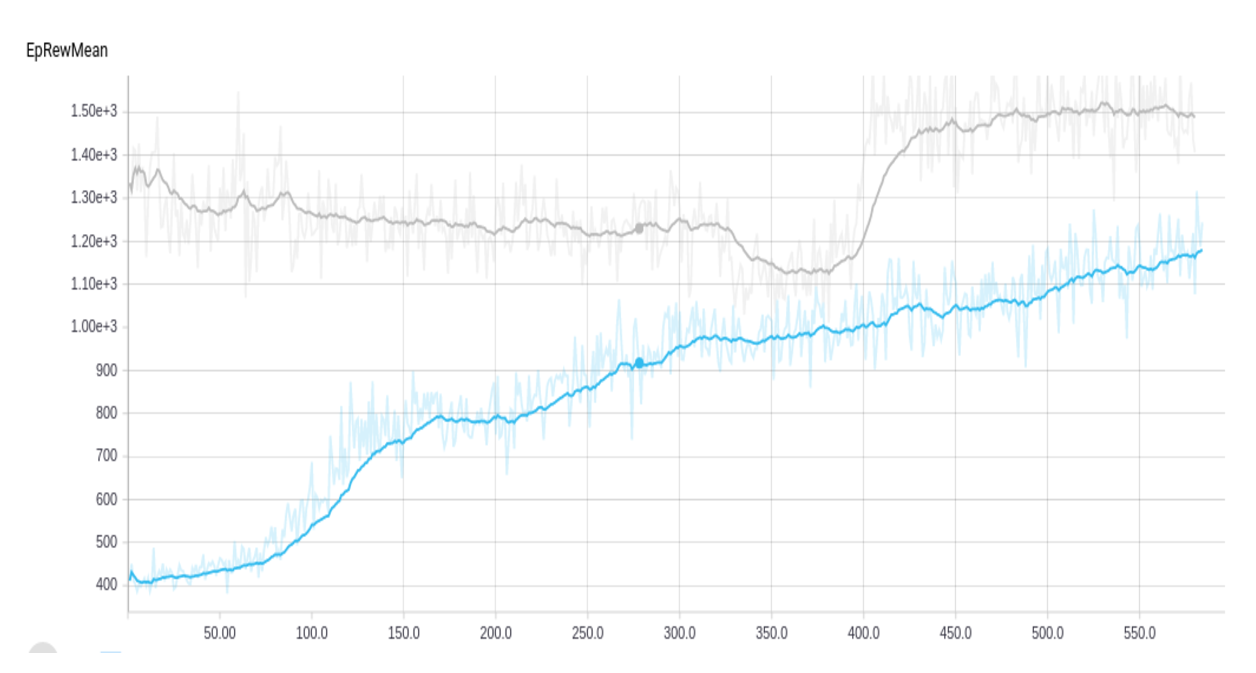
\includegraphics[width=0.8\textwidth]{Cap6/rnrrrrrewardcurve.eps}
	\caption{RNR+RRR Reward Curves by learning update. We trained in two sessions. The blue curve shows the first session and the gray one the second session.}
	\label{fig:rnrrrrrewardcurve}
\end{figure}

One fact that is interesting to mention: in RNR motion (without reference), the agent learns to kick with the right leg. In this model, on the other side, the agent learns to kick with the left leg, as in reference motion.

\begin{figure}[!htbp]
	\centering
	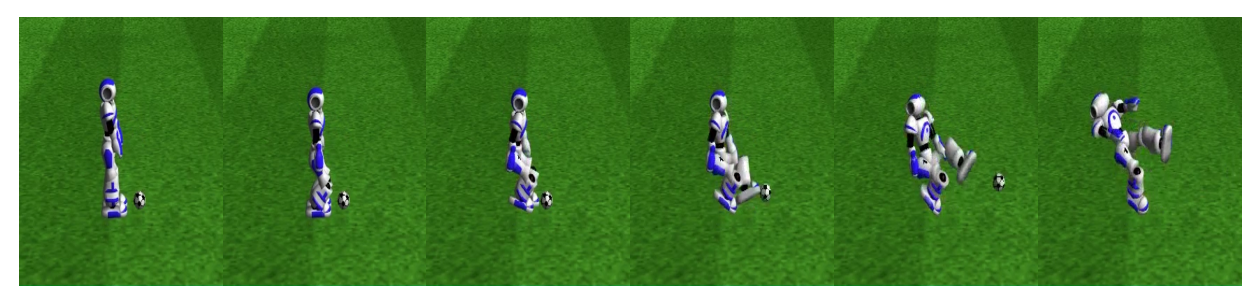
\includegraphics[width=0.8\textwidth]{Cap6/rnrrrrreward.eps}
	\caption{RNR+RRR Motion Sequence. In this model, the agent learns to kick with the left leg, as in reference.}
	\label{fig:rnrrrrreward}
\end{figure}


The big challenge of this model is to tune the weight parameter for each reward. If we use much greater reward for move the ball, the model collapses to RNR configuration. On the other side, if the reference reward is much greater, it collapses to RRR. It is a trade-off and is very difficult to tune this kind of parameter manually. Figure \ref{fig:rnrrrrtradeoff} shows a collapse case.


\begin{figure}[!htbp]
	\centering
	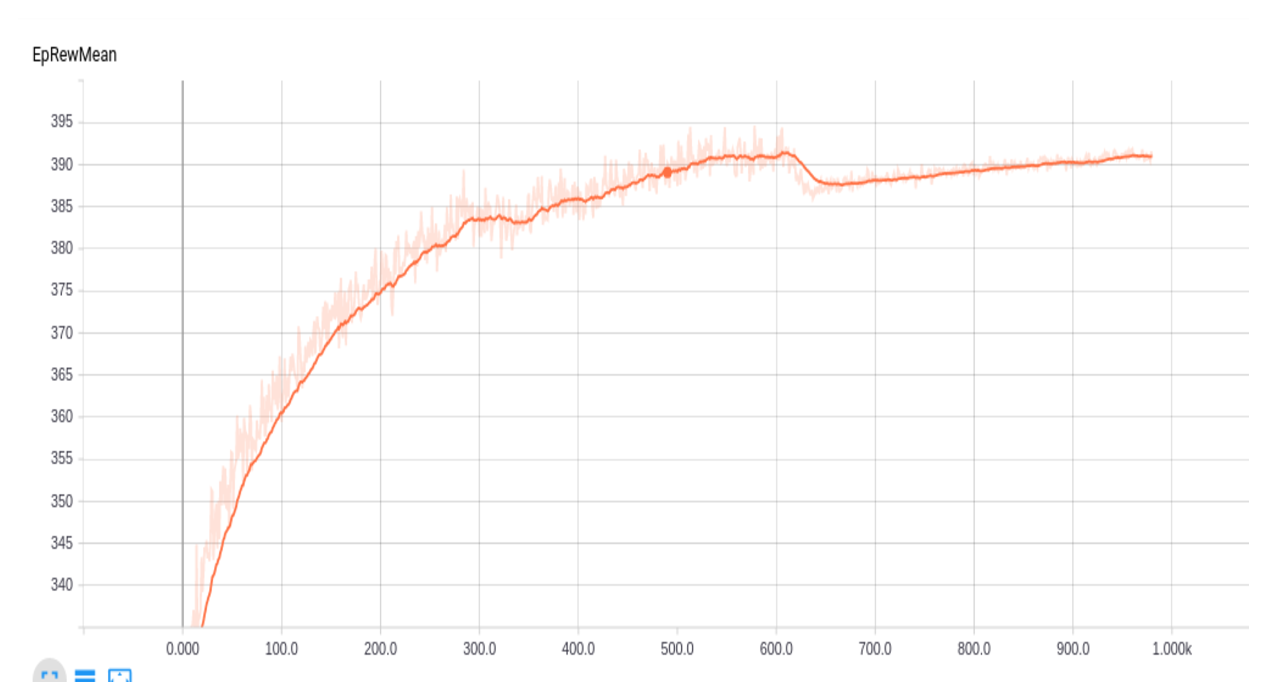
\includegraphics[width=0.8\textwidth]{Cap6/rnrrrrtradeoff.eps}
	\caption{Tradeoff between RNR and RRR models: when RRR is much greater, the models collpases to its model.}
	\label{fig:rnrrrrtradeoff}
\end{figure}

\subsection{RNR+RRR+RISD}

Even joining RNR and RRR, the agent is not able to learn the main patterns from the kick motion. It is difficult to learn, for example, that the leg should go back before making the move.

The main reason for this challenge -- even when we pass the reference motion -- is because the training is intrinsically sequential. It means that the later stages is achieve only if all previous states are satisfied. Otherwise, probably the agent will fall and not complete the episode.

Using the RISD model, we can train the whole motion "in parallel". We show the training curve from RNR+RRR+RISD model in Figure \ref{fig:rnrrrrrisdcurve}. 

\begin{figure}[!htbp]
	\centering
	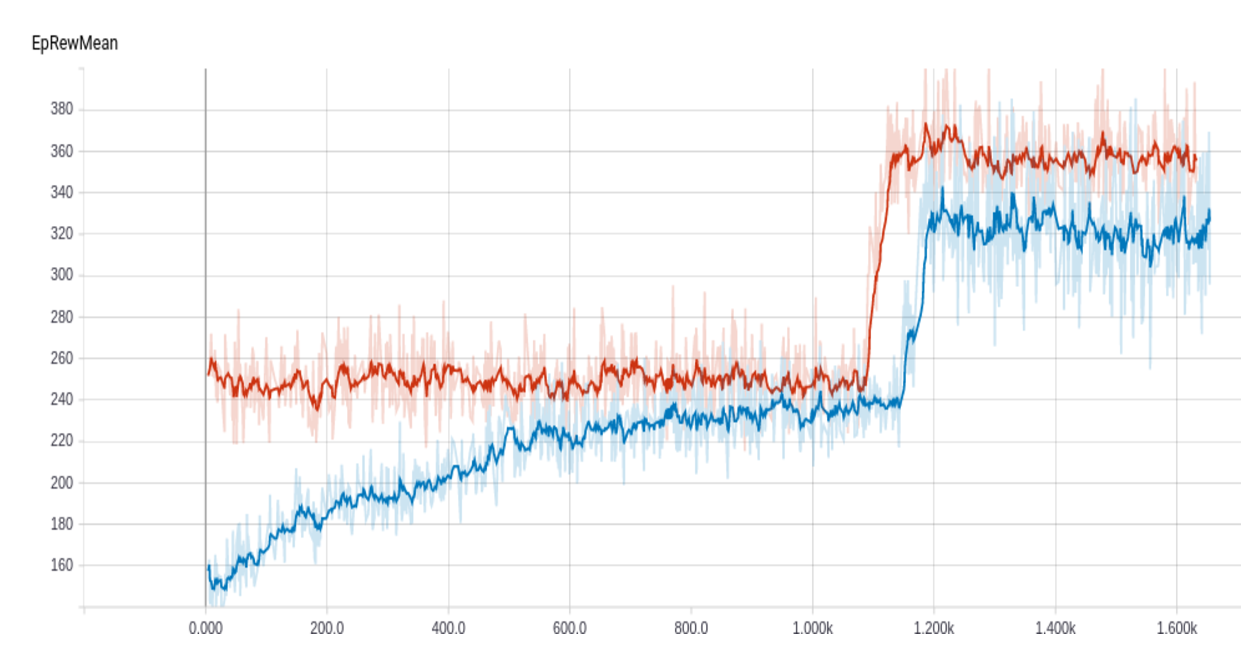
\includegraphics[width=0.8\textwidth]{Cap6/rnrrrrrisdcurve.eps}
	\caption{RNR+RRR+RISD learning curve in two sessions of training. The blue curve was the first session and the red one was the second.}
	\label{fig:rnrrrrrisdcurve}
\end{figure}


During the first session of training, the first thousand updates was related to reduce the error related to the reference motion. It is similar to the curve from RRR model. After this, the model grows drastically until a new baseline. It corresponds to the moment where the agent, by exploration, achieves the situation of completing the whole motion.

The second session starts from the first one. However, the first part of the training is comparable to the result before the drastic grow from first session. Then, by exploration, the reward drastically grows again, but for a second baseline, higher.

Comparing the result from both training, the second baselines is able to kick the ball following the reference motion; the first isn't.

Figure \ref{fig:risdmotionsequence} shows the motion sequence from RNR+RRR+RISD model. It is a complex and detailed motion. Although it is able to kick the ball, it is a rare situation and hardly ever achieves 3 meters. The big problem of this motion is the beginning: the agent fails in maintain a support foot. Nevertheless, the pure reinforcement method was able to mimic the human behavior of kicking.

\begin{figure}[!htbp]
	\centering
	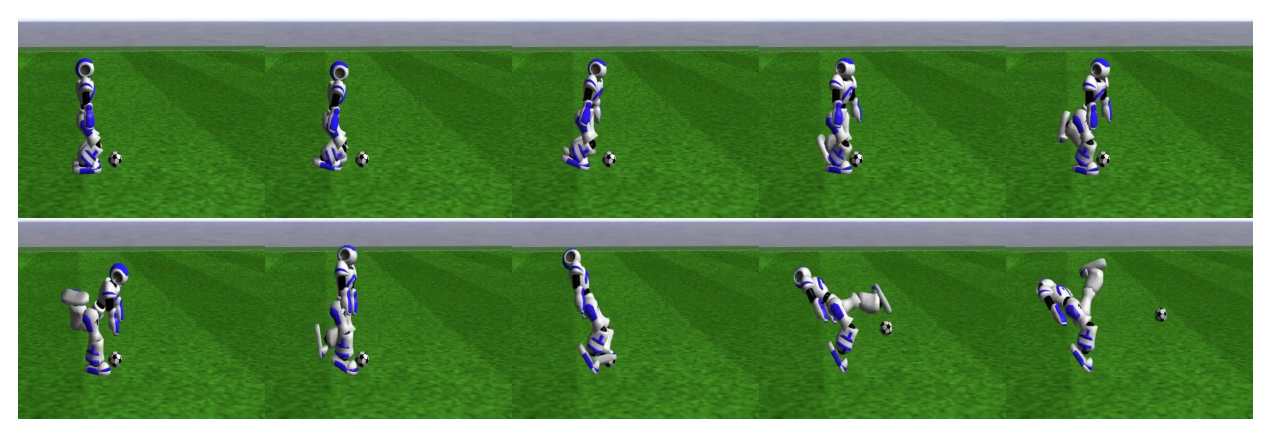
\includegraphics[width=0.8\textwidth]{Cap6/risdmotionsequence.eps}
	\caption{RNR+RRR+RISD motion sequence.}
	\label{fig:risdmotionsequence}
\end{figure}


\subsection{RNR+RRR+RISD+RET}

This final experiment using pure RL techniques tries to improve last model by using Early Termination. As we saw in Figure \ref{fig:rnrrrrrisdcurve}, the training curve is unstable and depends by the right situation of exploration to achieve a reasonable baseline. Considering the model, there is cases where the agent falls but we keep collecting data until the end of a fixed number of samples. Therefore, we collect a lot of wrong data that can harm learning.


\subsection{Reinforcement ``supervised"}\label{sec:suprl}

As a mid-term between pure RL techniques and HLM model, we propose a reinforcement ``supervised" learning model, where we use only the PPO algorithm but as initial stage we use the reference motions as a dataset $(x, y)$ where $x \in \mathcal{S}$ and $y \in \mathcal{A}$ and the reward is the opposite of mean absolute error:
\begin{equation}
R(x) = - \lvert \hat y(x) - y(x) \rvert 
\end{equation}

 In this way, we reduce RRR model to a ``supervised" problem without the simulation. This model breaks the sequentially of data, since the states are used in the training in isolation and not as a reflection of the horizon prior to this, satisfying Markov property.

Figure \ref{fig:rlsupcurves} shows the first of six training sessions for a reinforcement supervised configuration, using mean absolute error as penalization. It shows to be a bit difficult to converge -- the optimization is very sensible to learning rate value. In each training session, we needed to tune this hyperparameter again.

\begin{figure}[!htbp]
	\centering
	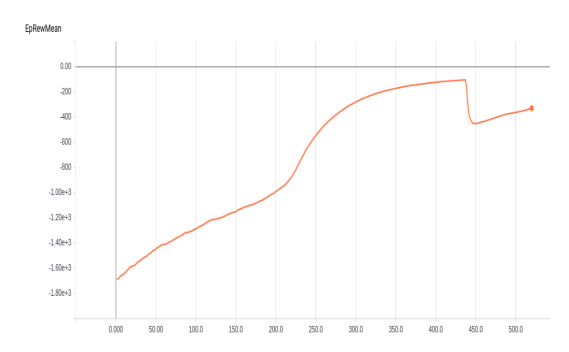
\includegraphics[scale=1.5]{Cap6/rlsuprewardcurves.eps}
	\caption{First session of training for reinforcement supervised model.}
	\label{fig:rlsupcurves}
\end{figure}

Although the learned motion mimics the reference, it accumulates error at the end of the motion and ends up kicking the floor, as shown in Figure \ref{fig:rlsupmotionsequence}. For this reason, it could not be used as seed for new kick policies.

\begin{figure}[!htbp]
	\centering
	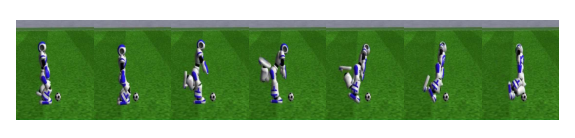
\includegraphics[scale=1.5]{Cap6/rlsupmotionsequence.eps}
	\caption{Motion sequence from reinforcement supervised learning agent.}
	\label{fig:rlsupmotionsequence}
\end{figure}

\subsection{Other ideas for pure RL techniques}

There are other possible ideas to explore in order to obtain a reasonable copy from the reference motion to use as seed for optimization. Analyzing the experiments described in this section until now, we found out we have two main problems:

\begin{itemize}
	\item The agent is not able to learning a stable support foot, compromising the later stages of kicking; and
	\item The kicking foot sometimes hits the ground and not the ball.
\end{itemize}

To address these problems, we need domain-specific rewards to ensure stability, such as:

\begin{itemize}
	\item Consider the pressure that support foot does on the ground; the more centralized is this pressure, the more stable kick should become;
	\item Consider the curve that kicking foot and leg do in relation to torso during reference motion; and
	\item Consider torso coordinates from reference motion during training.
\end{itemize}

We preferred not to explore these ideas because as we will see in next section, hybrid learning models worked much better and easier. Furthermore, in this work, we aim to explore non domain-specific techniques that could be generalized for other kinds of motions such as walking.

It worth mentioning that the techniques explored until now worked well, even not generating a seed for optimization. Fit this specific reference motion is really difficult because it has high performance and, therefore, the stability is a bit compromised. However, in other motions, they are good tooling for mimicking.

\section{Hybrid Learning Models}
In this section, we will explore an alternative for pure RL methods -- what we called Hybrid Learning Models. In this configuration, there is a pre-training step where we used supervised learning algorithms to fit the reference motion before use PPO algorithm.

\subsection{Supervised Learning Results}
\subsubsection{Training Results}

\begin{figure}[!htbp]
	\centering
	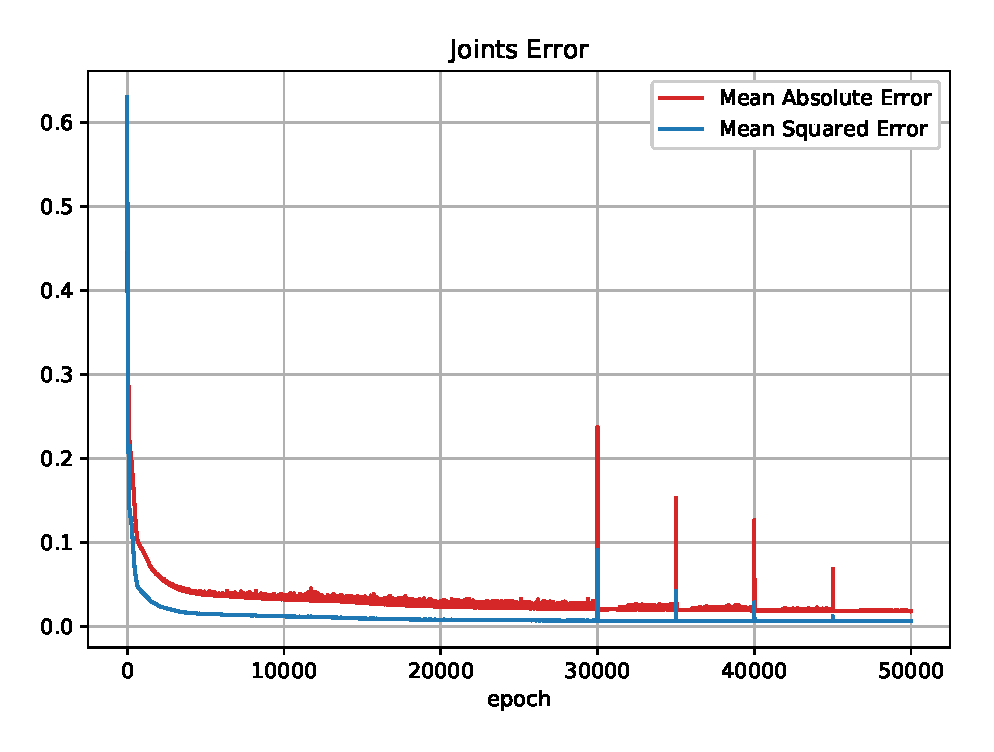
\includegraphics[width=1\textwidth]{Cap6/errors}
	\caption{Plots of mean squared error and mean absolute error, during training.}
	\label{fig:errors}
\end{figure}

The initial results came from the training procedure, outside the simulation environment. Figure \ref{fig:errors} presents training curves for the kick keyframe dataset. In this case, plots show the mean squared error and the mean absolute error metrics. In both metrics, the value drastically decreases in the first epochs. This same behavior was present in other training procedures as well. However, only after thousands of epochs, the network has achieved a low error that successfully reproduced the motion, which has shown how sensible to small joint errors keyframes were, given that they were open-loop motions. The peaks, during the training has happened at the learning rate transition instants, but they did not hurt the training procedure itself.

\subsubsection{The Learned Kick Motion}

The final mean absolute error was \textbf{0.018} radians and the motion was visually indistinguishable from the original one, as can be seen in Figure \ref{fig:motions}. In this figure, snapshots from both motions were taken. Figure \ref{fig:kick_joints_curves} shows several plots of joint angles, by comparing the original and learned kick motions. As we may see, the learned motion has fitted the movement with minor errors\footnote{\label{footnote_walk} Kick results video: https://youtu.be/UAbqQLUnvDo}.

\begin{figure}[!htbp]
	\centering
	\includegraphics[angle=90,width=1\textwidth]{Cap6/motions}
	\caption{The kick motion. The first row of figures shows the original kick motion. The second row shows the learned kick motion. Both motions are visually indistinguishable.}
	\label{fig:motions}
\end{figure} 

In order to evaluate the learned kick motion in the RoboCup Soccer 3D domain, we created a statistical test. Inside the test scenario, the ball was initially placed in the center of the field with an agent near to it. The only action of the agent was to kick the ball in the goal direction. After the kick, the agent run until reaching the ball and kicked it again, repeating this process till scoring a goal. When the goal has occurred, this same scenario was repeated. The whole test was conducted, during thirty minutes in clock time and the following data was collected: total number of kicks, number of successful kicks, mean distance that the ball has traveled, and the standard deviation of this measure. The results from the original and learned kicks is shown in Table \ref{tab_kicks_statistics}.


\begin{figure*}[!htbp]
	\centering
	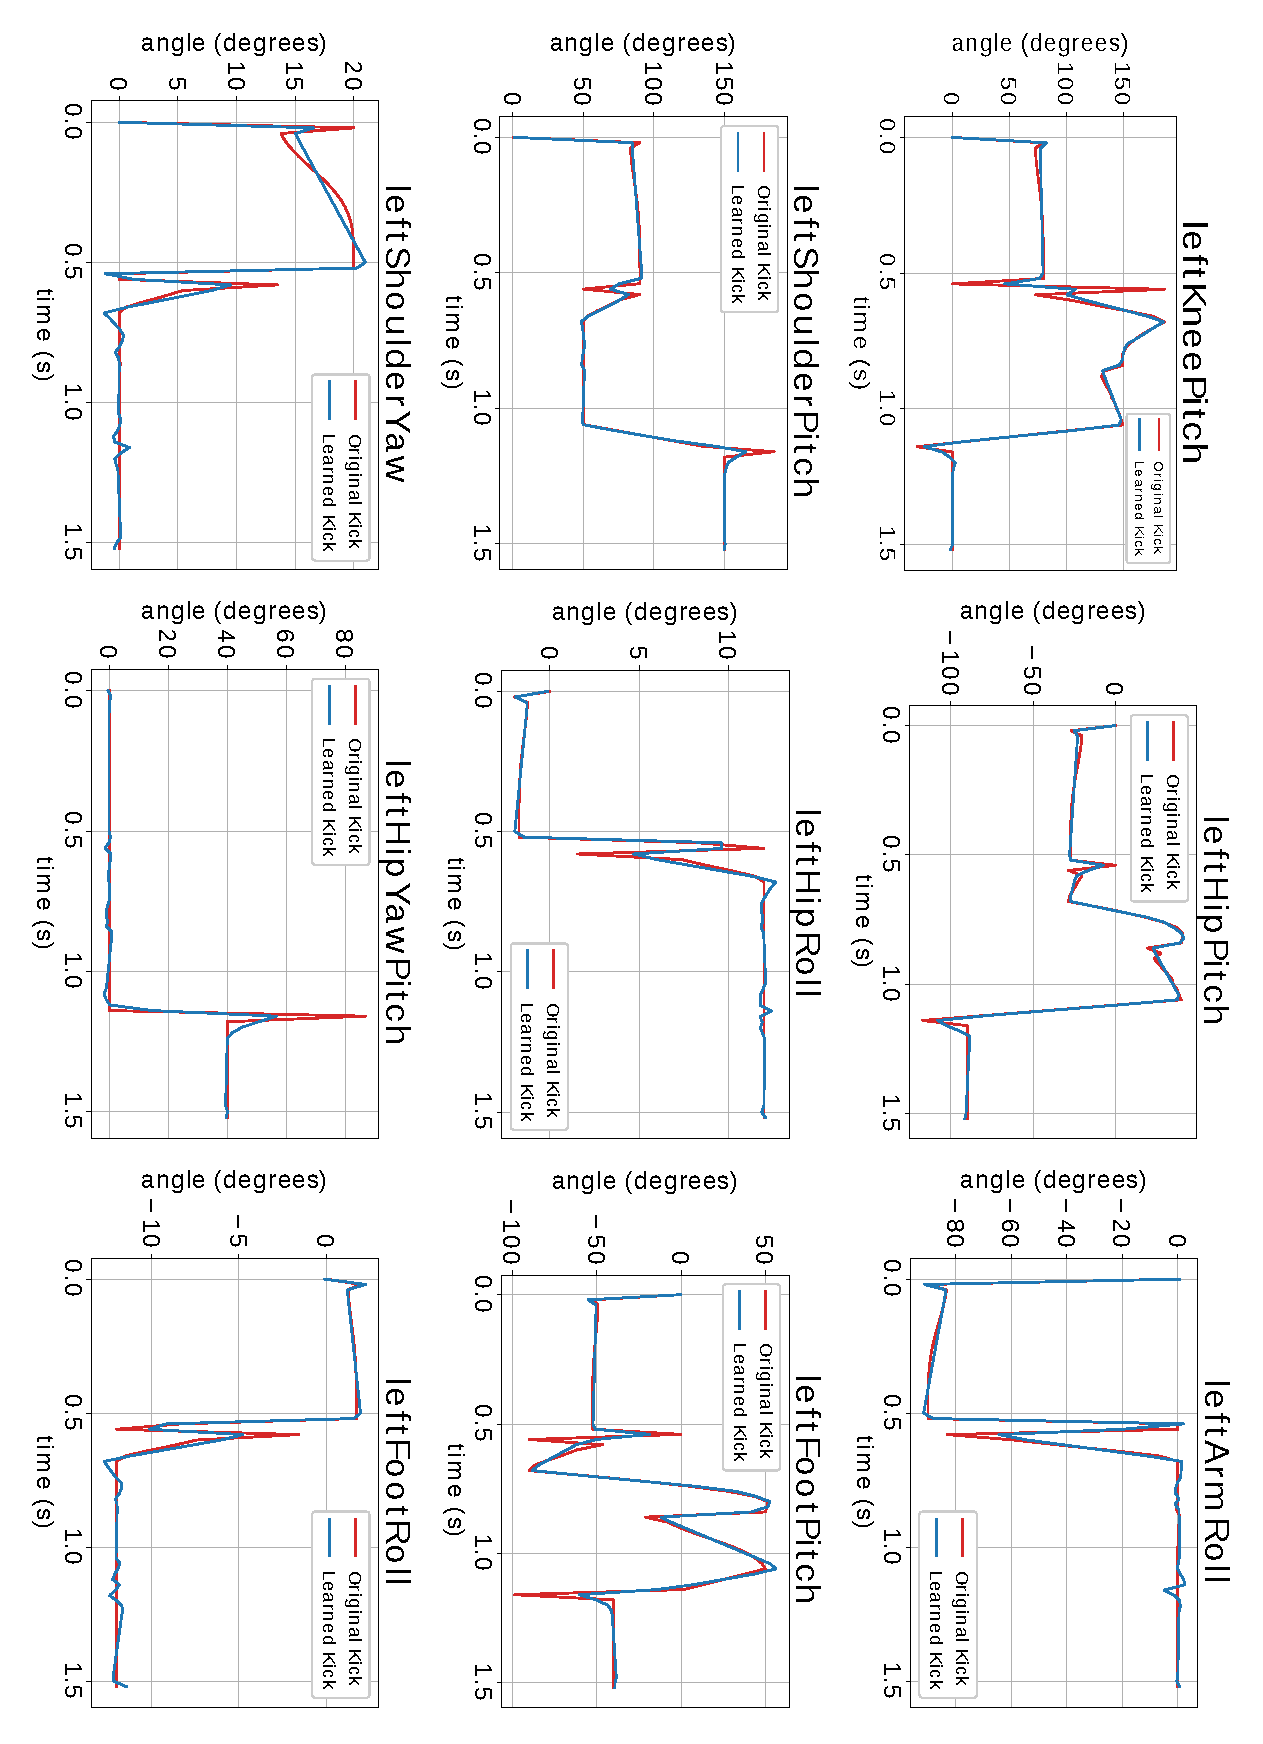
\includegraphics[angle=90,width=1\textwidth]{Cap6/kick_joints_curve}
	\caption{Joint values for comparing original and learned kicks. The neural network was able to fit the joint trajectories with small errors.}
	\label{fig:kick_joints_curves}
\end{figure*}


\begin{table}[htbp]
	\caption{The Kick Comparison}
	\begin{center} 
		\begin{tabular}{|c|c|c|c|}
			\hline
			\textbf{Kick}&\multicolumn{3}{|c|}{\textbf{Statistics}} \\
			\cline{2-4} 
			\textbf{Type} & \textbf{\textit{Accuracy (\%)}}& \multicolumn{2}{|c|}{\textbf{Distance (\(m\))}} \\ 
			\cline {3-4}
			& & \textbf{\textit{Mean}}& \textbf{\textit{Std}} \\
			\hline
			Original Kick & 64.5 & 8.92 & 3.82  \\
			\hline
			Neural Kick & 52.6 & 7.16 & 4.06 \\
			\hline
		\end{tabular}
		\label{tab_kicks_statistics}
	\end{center}
\end{table}

Although both kicks had similar results, the original kick was slightly better in this scenario. By confronting Figure \ref{fig:kick_joints_curves}, we can conclude that even with an almost equal representation, the kick lost part of its efficiency and this fact has shown how sensible were movements based on keyframe data.

\subsubsection{The Learned Walk Motion}
By using the modified server described in Subsec. \ref{AA}, a dataset with samples of the UT Austin Villa's walking motion \cite{macalpine2013} was acquired. This team is the current champion of the RoboCup Soccer 3D competition \cite{macalpine2017}.

The objective was to mimic the walk motion as a keyframe and has used that in our agent. The previously described framework for learning our own kick motion was used in this training, by including the neural network architecture and its hyperparameters.

The results from this training are shown in Figure \ref{fig:walk_joints_curves}. Similarly to Figure \ref{fig:kick_joints_curves}, it shows the joint angles throughout the walking motion period for the original and learned walk. Additionally, it shows the real joints values from the movement in the server. These joints were chosen because they were the most dynamic in the walk motion and, therefore, the hardest to learn.

\begin{figure*}[!htbp]
	\centering
	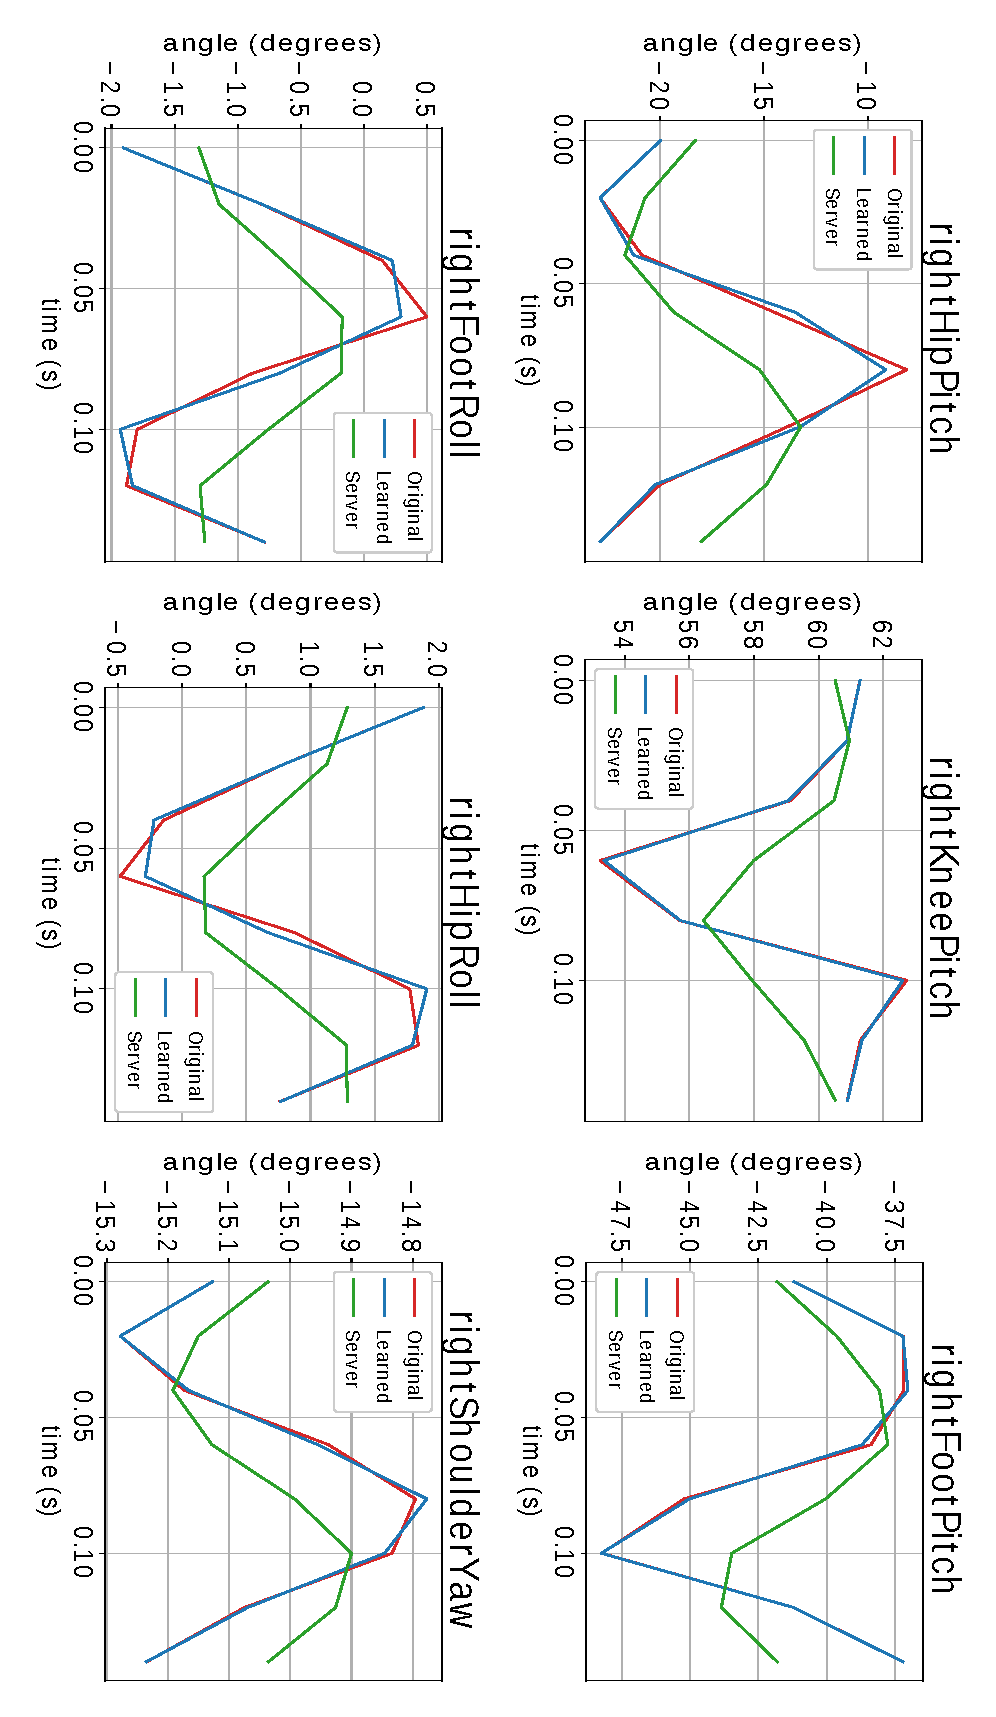
\includegraphics[angle=90,width=1\textwidth]{Cap6/walk_joints_curves}
	\caption{Joints positions, during a period of the walking motion for the original walk, and the learned walk and the joints positions effectively attained, during the learned walking motion.}
	\label{fig:walk_joints_curves}
\end{figure*}

The learned motion has fitted the dataset very well. However, these values were just desired joints. In fact, these values were used as references to joint controllers and were also attenuated due to joint dynamics. Furthermore, this motion was operated in a open-loop fashion, so the agent was not able to correct its own trajectory, and this walks got biased within the simple task of walking straight forward.

Despite the facts previously described, the motion has worked well in a non-competitive scenario\footnote{\label{footnote_walk} Walk results video: https://youtu.be/-pHxTrxllyY}, which was shown in the metrics collected from the Forward Walk test scenario -- agent walking forward from the goal post until the center line of the field -- in Table \ref{tab_walk} and the visual representation in Figure \ref{fig:walkings}.

\begin{table}[htbp]
	\caption{Walk Comparison - Forward Walk}
	\begin{center}
		\begin{tabular}{|c|c|c|c|c|}
			\hline
			\textbf{Walk}&\multicolumn{4}{|c|}{\textbf{Statistics}} \\
			\cline{2-5} 
			\textbf{Type} &\multicolumn{2}{|c|}
			{\textbf{Velocity \((m/s)\)}}
			&\multicolumn{2}{|c|}{\textbf{Y Error \( (m) \) }} \\ 
			\hline
			&
			\textbf{\textit{Mean}} &
			\textbf{\textit{Std}} & \textbf{\textit{Mean}} & \textbf{\textit{Std}} \\
			\hline
			Original Walk & 0.87 & 0.01 & - & -  \\
			\hline
			Learned Walk & 0.23 & 0.01 & 0.96 & 2.63 \\
			\hline
		\end{tabular}
		\label{tab_walk}
	\end{center}
\end{table}


\begin{figure}[!htbp]
	\centering
	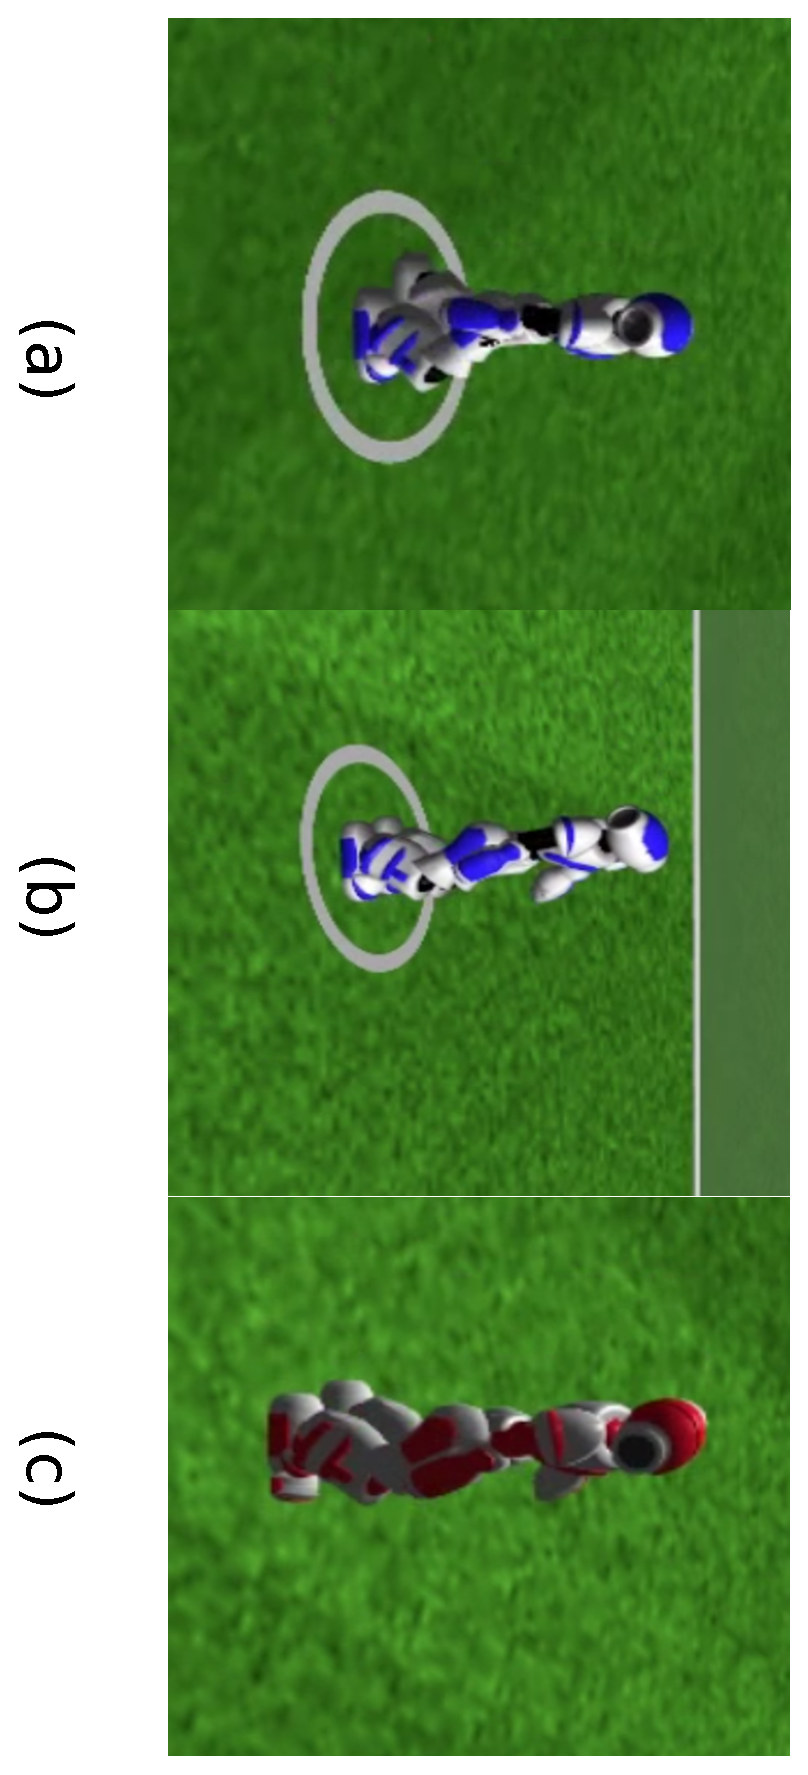
\includegraphics[angle=90, width=1\textwidth]{Cap6/walkings}
	\caption{The walking motions comparison. Figure (a) shows our agent in its regular walk, Figure (b) shows the same agent mimicking UT Austin Villa walk, and Figure (c) shows the UT Austin Villa agent itself performing his own walking motion.}
	\label{fig:walkings}
\end{figure}

\subsubsection{Other motions}

This same framework was used to learn other keyframe motions originated from our agent itself, such as the get up motion. As the cases previously described, the resultant neural network was capable of mimicking the keyframe, by including its interpolation. Hence, all of our keyframe motions could be replaced by neural motions with similar performance.

However, the huge improvement of this method was about mimicking other teams motions. In the Soccer 3D environment, movements like kick and walking have giant impact in team's performance. With this learning framework, our agent was able to mimic multiples movements from several teams.

As an example, we have collected data from UT Austin Villa kick, which was originally optimized by using Deep Reinforcement Learning techniques \cite{mcalpine2017}. Our agent has learned this kick without any additional optimization strategy: we just have used samples collected from the modified server.


\subsection{HLM+RNR}


\subsection{Final Model: HLM+RNR+RET}\label{sec:hlmrnrret}
As final model to explore, we addressed HLM+RNR with Early Termination technique. As described earlier in this work, without it, we collect data that potentially harm training.

In this case, Early Termination consists in end up the episode in two scenarios:

\begin{itemize}
	\item When the robot falls and, therefore, it can't recover itself; and
	\item When robots kicks the ball, all actions after it will not affect the reward; it is a way to make this reward "less delayed".
\end{itemize}

In terms of RL training, we did two sessions.

 In the first one, we parameterized RNR in a way to mainly improve the velocity in frontal direction. The parameters can be found in Appendix \ref{ap:hyperparameters}. Figure \ref{fig:hlmretsess1} shows the reward curve. It results in a kick that optimizes the main problem from the original kick: accuracy. As you can see in Table \ref{tab_kicks_statistics}, the keyframe kick has low accuracy and the learned one is worse, due to the intrinsic error from learning process. At the end of this first session of RL training, the agent is able to improve its accuracy, although the mean distance being low. Numeric results will be described in next subsection.
 
 
 
 \begin{figure}[!htbp]
 	\centering
 	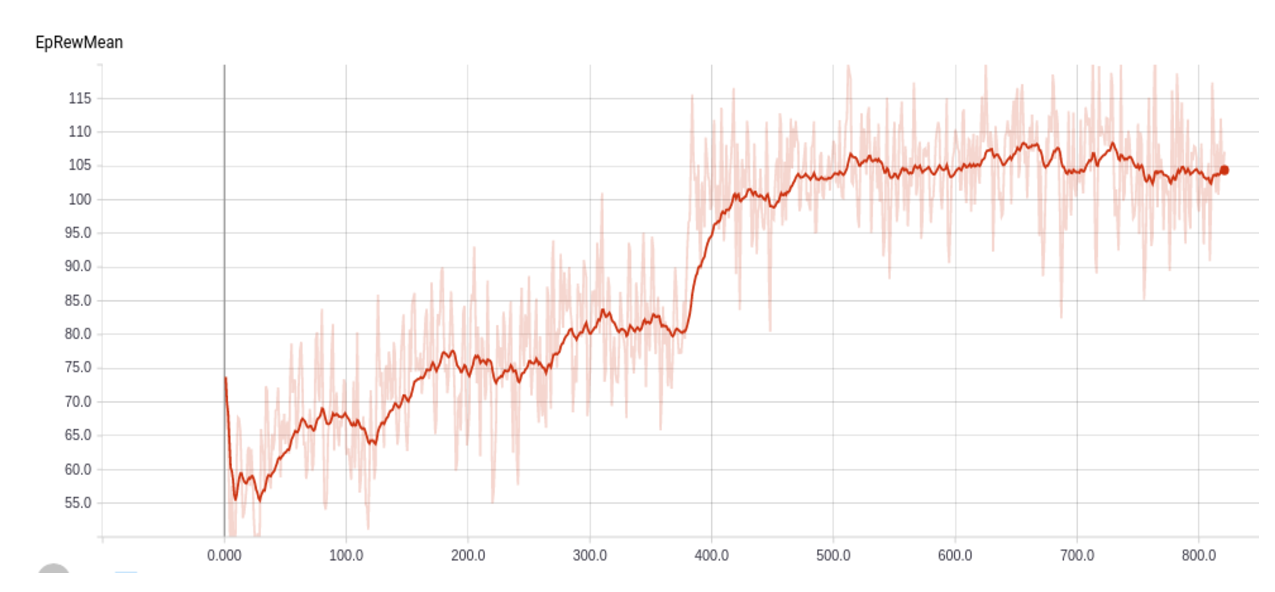
\includegraphics[ width=1\textwidth]{Cap6/hlmretsess1.eps}
 	\caption{The reward curve from the first session of HLM+RNR+RET model.}
 	\label{fig:hlmretsess1}
 \end{figure}

Figure \ref{fig:hlmretsess1motseq} shows the motion sequence after this first session. Although the agent kicks the ball, there is no gain in height. This is a problem for two reasons: first, in a game situation, the ball probably will hits an opponent; second, there is friction between the ball and ground, decreasing the final reach of it.

 

\begin{figure}[!htbp]
	\centering
	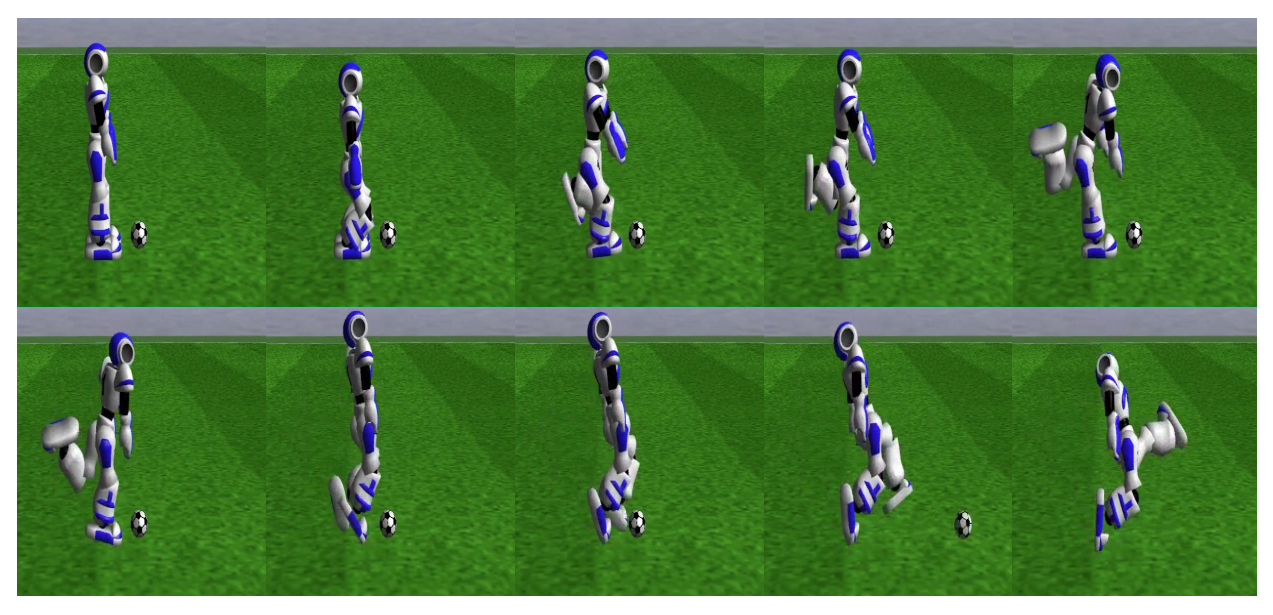
\includegraphics[ width=1\textwidth]{Cap6/hlmretsess1motseq.eps}
	\caption{HLM+RNR+RET motion sequence after first session of training.}
	\label{fig:hlmretsess1motseq}
\end{figure}
 
 In the second session, on the other side, we gave preference to kicks with height, positively reinforcing z-axis velocity. Figures \ref{fig:hlmretsess2} and \ref{fig:hlmretsess2motseq} shows the reward curve and motion sequence, respectively. Even not being so different from motion sequence of Figure \ref{fig:hlmretsess1motseq}, this training made the agent hits the ball in a way that it gains height, as shown if Figure \ref{fig:hlmretsess2motseq}, resulting in a better general performance than the original keyframe kick.
 
  
 \begin{figure}[!htbp]
 	\centering
 	\includegraphics[ width=1\textwidth]{Cap6/hlmretsess2}
 	\caption{The reward curve from the second session of HLM+RNR+RET model.}
 	\label{fig:hlmretsess2}
 \end{figure}
 
 \begin{figure}[!htbp]
 	\centering
 	\includegraphics[ scale=0.8]{Cap6/hlmretsess2motseq}
 	\caption{HLM+RNR+RET motion sequence after second training session.}
 	\label{fig:hlmretsess2motseq}
 \end{figure}

\subsection{Kick Behavior: Numerical Results}

We created a last test scenario, similar to that from Table \ref{tab_kicks_statistics}, where the agent started 2 meters from the ball and approaches to it and finally kick the ball. This process is conducted by Kick Behavior, a high-level agent behavior that integrates the walk and kick motions. The idea behind this is try to simulate better in-game situation and check if the model obtained by these optimizations generalizes well to high-level behaviors, given that we didn't optimize any parameter regarding to ball approaching or waking motion.

We collected the distance traveled by ball in axis $x$ and $y$, and the maximum height achieved by ball during its travel. We also defined a concept of accuracy, considering a "wrong" kick when the ball doesn't achieve at least 0.5 meters per second. We ran a hundred of samples and calculated accuracy and mean and standard deviation from other features.

In Table \ref{tab:finaltest}, we compare four different kicks:

\begin{itemize}
	\item \textbf{Original Kick}: The keyframe kick used as reference motion;
	\item \textbf{Learned Kick}: The neural network we learned by supervised learning and using as dataset Original Kick;
	\item \textbf{HLM+RNR+RET Kick}: The Hybrid Learning Model proposed in subsection \ref{sec:hlmrnrret}.
\end{itemize}

\begin{table}[!htbp]
	\caption{Kick Comparison - General Evaluation}
	\begin{center} 
		\begin{tabular}{|c|c|c|c|c|c|}
			\hline
			\textbf{Kick}&\multicolumn{5}{|c|}{\textbf{Statistics}} \\
			\cline{2-6} 
			\textbf{Type} & \textbf{\textit{Accuracy (\%)}}& \multicolumn{2}{|c|}{\textbf{Distance X(\(m\))}}& 
			\multicolumn{2}{|c|}{\textbf{Distance Z (\(m\))}}\\
			\cline {3-6} 
			& & \textbf{\textit{Mean}}& \textbf{\textit{Std}}
			& \textbf{\textit{Mean}}& \textbf{\textit{Std}}\\
			\hline
			Original Kick & 69.0 & 6.27 & 5.03 & 0.16 & 0.41 \\
			\hline
			Learned Kick & 63.0 & 3.06 & 4.22 & 0.09 & 0.17 \\
			\hline
			\textbf{HLM+RNR+RET Kick}  & \textbf{92.0} & \textbf{7.60} & \textbf{3.71} & \textbf{0.45} & \textbf{0.49}  \\
			\hline
		\end{tabular}
		\label{tab:finaltest}
	\end{center}
\end{table}

As Table \ref{tab:finaltest} shows, HLM+RNR+RET kick outperforms both original and learned ones, in this test scenario. General Evaluation means considering the distance traveled by all kicks, even the ones considered ``wrong".

However, it worth mentioning the Effective Evaluation: consider the distance just from ``right" kicks. We show this evaluation in Table \ref{tab:finaltesteff}.

\begin{table}[!htbp]
	\caption{Kick Comparison - Effective Evaluation}
	\begin{center} 
		\begin{tabular}{|c|c|c|c|c|}
			\hline
			\textbf{Kick}&\multicolumn{4}{|c|}{\textbf{Statistics}} \\
			\cline{2-5} 
			\textbf{Type} &  \multicolumn{2}{|c|}{\textbf{Distance X(\(m\))}}& 
			\multicolumn{2}{|c|}{\textbf{Distance Z (\(m\))}}\\
			\cline {2-5} 
			& \textbf{\textit{Mean}}& \textbf{\textit{Std}}
			& \textbf{\textit{Mean}}& \textbf{\textit{Std}} \\
			\hline
			Original Kick  & \textbf{9.05} & \textbf{3.44} & 0.21 & 0.49 \\
			\hline
			Learned Kick  & 4.82 & 4.46 & 0.12 & 0.21 \\
			\hline
			\textbf{HLM+RNR+RET Kick} & \textbf{8.26} & \textbf{3.09} & \textbf{0.48} & \textbf{0.49}  \\
			\hline
		\end{tabular}
		\label{tab:finaltesteff}
	\end{center}
\end{table}

We can see from Table \ref{tab:finaltesteff} that when considering just right kicks, the performance from Original Kick is slightly better. This can be explained by \textbf{performance-stability tradeoff}: the better the performance is, the worse stability should become. However, our training, in terms of cumulative reward, is better always kick. Therefore, the training sacrifices performance to gain accuracy -- which is also better in terms of competition as well.

\chapter{Conclusions, Recommendations, and Future Works}\label{ch:conclusion}
\section {Preliminary Conclusions and Future Works}

In this work, we presented a method for learning humanoid robot movements using datasets composed of joint values at each time instant. The provided learning framework was capable to learn several types of motion, including walk and kick, without any change in network architecture or hyperparameters.

Moreover, the learned motions had similar performance to the original ones. Furthermore, this framework was able to learn from other teams motions, without any knowledge about the underlying implementation -- only by using the joints values provided by a modified version of the server. This was a huge improvement, in terms of getting improved motions, as our agent was able to mimic other teams motions, by using this machine learning technique.

As future works, we plan to apply Deep Reinforcement Learning algorithms to obtain faster and more robust kicks, by using as a "seed" the neural network obtained from this work.

Another track to be followed is to transfer the learning of this obtained network to a new network that represents the motion policy itself (i.e a network which has as inputs the current state of the robot, by including joint and link states, besides the current time instant), optimizing this motion policy, in order to get a closed-loop walking and kicking motion that can correct itself.

Finally, as a long term goal, we intend to create some model-free walking and kicking engines.

\section{The Activities Plan}

As next steps of this work, we plan to:

\begin{enumerate}
\item Import our supervised policy model into Deep Reinforcement Learning algorithms -- Expected to be finished until the end of \textbf{June, 2018};
\item Iterate over objective function construction and optimization, in order to improve the kick motion -- Expected to be finished until mid \textbf{August, 2018};
\item Execute the same test scenarios previously applied to compare results -- Expected to be finished until the end of \textbf{August, 2018}; 
\item Test in 11 x 11 game to compare team performance -- Expected to be finished until the end of \textbf{August, 2018}; and
\item Complement this work with some novel background, methodology, results, and conclusions -- Expected to be finished until \textbf{November, 2018}.
\end{enumerate}


% REFERENCIAS BIBLIOGRAFICAS
\renewcommand\bibname{\itareferencesnamebabel} %renomear título do capítulo referências
\bibliography{Referencias/referencias}

% Apendices
%\appendix
%\chapter{Topicos de Dilema Linear} %opcional
%
\begin{table}[!htbp]
	\caption{Hyperparameters - RNR, RRR, RNR+RRR, RNR+RRR+RISD}
	\begin{center} 
		\begin{tabular}{|c|c|c|c|c|c|}
			\hline
			Hyperparameter & Value   \\
			\hline
			Learning Rate &    $10^{-3}$    \\
			Timesteps per Actorbatch & 4096    \\
			Batch Size &   256     \\
			Epochs &  10\\
			$\gamma$ & 0.99 \\
			$\lambda$ & 0.95 \\
			Timesteps (Total) & $8 \times 10^{8}$ \\
			Clip Parameter & 0.2\\
			Entropy Coefficient & 0.0 \\
			RNR Parameters Vector  & $\begin{bmatrix}
				1.0 & -0.3 & 2.0
			\end{bmatrix}$\\
			RRR Parameters Vector  & $\begin{bmatrix}
			1.0 & 1.0 & 2.0 & 2.0 & 2.0 & 1.0 & 2.0 & 2.0 & 2.0 & \\ 1.0 & 5.0 & 5.0 & 5.0 & 5.0 & 5.0 & 5.0 & 3.0 &\\ 3.0 & 3.0 & 3.0 & 3.0 & 3.0 
			\end{bmatrix}$\\
			\hline
		\end{tabular}
	
		\label{tab:finaltest}
	\end{center}
\end{table}


\begin{table}[!htbp]
	\caption{Hyperparameters - Reinforcement ``supervised" - First Session}
	\begin{center} 
		\begin{tabular}{|c|c|c|c|c|c|}
			\hline
			Hyperparameter & Value   \\
			\hline
			Learning Rate &    $10^{-4}$    \\
			Timesteps per Actorbatch & 4096    \\
			Batch Size &   256     \\
			Epochs &  10\\
			$\gamma$ & 0.99 \\
			$\lambda$ & 0.95 \\
			Timesteps (Total) & $10^{6}$ \\
			Clip Parameter & 0.2\\
			Entropy Coefficient & 0.0 \\
			\hline
		\end{tabular}
		
		\label{tab:finaltest}
	\end{center}
\end{table}

\begin{table}[!htbp]
	\caption{Hyperparameters - HLM+RNR, HLM+RNR+RET - First Session}
	\begin{center} 
		\begin{tabular}{|c|c|c|c|c|c|}
			\hline
			Hyperparameter & Value   \\
			\hline
			Learning Rate &    $10^{-6}$    \\
			Timesteps per Actorbatch & 4096    \\
			Batch Size &   2048     \\
			Epochs &  10\\
			$\gamma$ & 0.99 \\
			$\lambda$ & 0.95 \\
			Timesteps (Total) & $4 \times 10^{6}$ \\
			Clip Parameter & 0.2\\
			Entropy Coefficient & 0.0 \\
			RNR Parameters Vector  & $\begin{bmatrix}
			1.0 & -0.3 & 2.0
			\end{bmatrix}$\\
			\hline
		\end{tabular}
		
		\label{tab:finaltest}
	\end{center}
\end{table}


% Anexos
%\annex
%\chapter{Exemplo de um Primeiro Anexo} %opcional
%% Texto do Primeiro Anexo
\section{Uma Seção do Primeiro Anexo}
% Texto da primeira secao do primeiro anexo
Algum texto na primeira seção do primeiro anexo.



% Glossario
%\itaglossary
%\printglossary

% Folha de Registro do Documento
% Valores dos campos do formulario
\FRDitadata{June 12th, 2018}
\FRDitadocnro{DCTA/ITA/DM-018/2015} %(o número de registro você solicita a biblioteca)
\FRDitaorgaointerno{Aeronautics Institute of Technology -- ITA}
%Exemplo no caso de pós-graduação: Instituto Tecnol{\'o}gico de Aeron{\'a}utica -- ITA
\FRDitapalavrasautor{Deep Reinforcement Learning; Robotics; Artificial Intelligence}
\FRDitapalavrasresult{Deep Reinforcement Learning; Robotics; Artificial Intelligence}
%Exemplo no caso de graduação (TG):
%\FRDitapalavraapresentacao{Trabalho de Graduação, ITA, São José dos Campos, 2015. \NumPenultimaPagina\ páginas.}
%Exemplo no caso de pós-graduação (msc, dsc):
\FRDitapalavraapresentacao{ITA, São José dos Campos, 2018. Trabalho de Graduação.}
\FRDitaresumo{Controlling a high degrees of freedom humanoid robot is acknowledged as one of the hardest problems in Robotics. Due to the lack of mathematical models, an approach frequently employed is to rely on human intuition to design keyframe movements by hand, usually aided by graphical tools. In this paper, we propose a learning framework based on neural networks in order to mimic humanoid robot movements. The developed technique does not make any assumption about the underlying implementation of the movement, therefore both keyframe and model-based motions may be learned. The framework was applied in the RoboCup 3D Soccer Simulation domain and promising results were obtained using the same network architecture for several motions, even when copying motions from another teams.}
%  Primeiro Parametro: Nacional ou Internacional -- N/I
%  Segundo parametro: Ostensivo, Reservado, Confidencial ou Secreto -- O/R/C/S
\FRDitaOpcoes{N}{O}
% Cria o formulario
\itaFRD

\end{document}
% Fim do Documento. O massacre acabou!!! :-)
